\chapter{Vektoranalysis}
\label{\detokenize{vektoranalysis/vektoranalysis:vektoranalysis}}\label{\detokenize{vektoranalysis/vektoranalysis::doc}}
\par
In diesem Kapitel der Vorlesung führen wir wichtige Konzepte der \emph{Vektoranalysis} ein.
Insbesondere schaffen wir die mathematischen Grundlagen für eine spezielle Art der mehrdimensionalen Integration, das Integrieren über sogenannte \emph{Untermannigfaltigkeiten} des \(\R^n\).
Um diese Integration durchführen zu können, entwickeln wir das Kalkül der \emph{Differentialformen} auf Mannigfaltigkeiten.

\par
Dieses Kalkül lässt auch den geometrischen Gehalt physikalischer Theorien wie Elektrodynamik oder Allgemeine Relativitätstheorie klar hervortreten.
So lassen sich beispielsweise die Maxwellschen Gleichungen der Elektrodynamik mit Hilfe des Differentialformenkalkül elegant beschreiben.

\par
Als zusätzliche Literatur und Referenz für diese Thematiken empfehlen wir das Buch von Agricola und Friedrich \cite{AF13}.


\section{Multilinearformen}
\label{\detokenize{vektoranalysis/multilinear:multilinearformen}}\label{\detokenize{vektoranalysis/multilinear:s-multilinearformen}}\label{\detokenize{vektoranalysis/multilinear::doc}}
\par
In diesem Abschnitt wollen wir die Definition der sogenannten \emph{Multilinearformen} einführen.
Für beliebige Vektorräume \(\V, W\) über einem Körper \(\K\) haben Sie bereits den Begriff der \emph{Linearform}, also einer linearen Abbildung \(\varphi:\V\rightarrow W\) kennengelernt.
Die Idee der Multilinearform ist anstatt nur einem, gleich \(k\) viele Vektorräume \(V_1,\ldots,V_k\) für \(k \in \N\) über \(\K\) zu betrachten und das Konzept der Linearität auf eine Abbildung \(\varphi:\V_1\times\ldots\V_k\rightarrow W\) zu übertragen.

\par
Zur Vereinfachung werden wir im Folgenden nur den Körper \(\K=\R\) betrachten, in den meisten Fällen lassen sich die hier beschriebenen Konzepte aber direkt auf allgemeine Körper übertragen.
Wir beginnen zunächst mit einer Wiederholung und betrachten die schon bekannten Linearformen.
Insbesondere soll der nächste Abschnitt die verschiedenen Begriffe des Dualraums abgrenzen.


\subsection{Dualräume}
\label{\detokenize{vektoranalysis/multilinear:dualraume}}
\par
Für einen reellen Vektorraum \(\V\) wollen wir lineare Abbildungen \(\varphi:V\to\R\) betrachten.
Diese lassen sich mit Hilfe der folgenden Definition zum algebraischen Dualraum zusammenfassen.
\begin{definition}{(Algebraischer Dualraum)}{vektoranalysis/multilinear:def:algebraischerDualraum}



\par
Es sei \(\V\) ein beliebiger \(\R\) Vektorraum.
Dann nennen wir die Menge
\begin{align*}
\V^\ast := \{\varphi:\V\rightarrow\R: \varphi\text{ ist linear}\}
\end{align*}
\par
den \textbf{algebraischer Dualraum} zu \(V\).
\end{definition}

\par
Aus \cite{Ten21} ist bereits der Begriff des \emph{topologischen Dualraums} bekannt, welcher allerdings eine etwas restriktivere Definition hat.
Sie fordert nämlich noch zusätzlich die Stetigkeit der linearen Abbildungen.
\begin{definition}{(Topologischer Dualraum)}{vektoranalysis/multilinear:def:topologischerDualraum}



\par
Es sei \(\V\) ein normierter \(\R\) Vektorraum für einen Körper \(\R\).
Dann nennen wir die Menge
\begin{align*}
\V^\prime := \{\varphi:\V\rightarrow\R: \varphi\text{ ist linear und stetig}\}
\end{align*}
\par
den \textbf{topologischer Dualraum} zu \(V\).
\end{definition}

\begin{emphBox}{}{}
\par
Der algebraische Dualraum ist im Allgemeinen nicht gleich dem topologischen Dualraum.
Der Hauptzweck dieses Abschnitts ist es diese Tatsache klar zu machen und die Unterschiede der beiden Definitionen herauszustellen.
\end{emphBox}

\par
Der Integraloperator ist ein typisches Beispiel für einen linearen stetigen Operator.
\begin{example}{(Integraloperator)}{vektoranalysis/multilinear:example-2}



\par
Es sei \(\V := C([0,1])\) der Funktionenraum der stetigen Funktionen auf dem Intervall \([0,1] \subset \R\).
Dann ist der durch \(T \colon C([0,1]) \rightarrow \R\) definierte Integraloperator mit
\begin{align*}
T(f) := \int_0^1 f(x) \, \mathrm{d}x
\end{align*}
\par
ein Element des \emph{topologischen Dualraums}, d.h. \(T \in \V^\prime\), da man zeigen kann, dass er linear und stetig ist.
\end{example}

\par
Folgende Bemerkung sagt etwas über die minimale Struktur, die der Vektorraum \(V\) haben muss, damit die Definition des topologischen Dualraums sinnvoll ist.
\begin{remark}{}{vektoranalysis/multilinear:remark-3}



\par
Damit die \cref{vektoranalysis/multilinear:def:topologischerDualraum} sinnvoll ist, ist es in der Tat nicht notwendig, dass \(V\) ein normierter Raum ist. Es reicht anzunehmen, dass \(\V\) ein \emph{topologischer Vektorraum} ist.
\end{remark}

\par
Durch Vergleichen von \cref{vektoranalysis/multilinear:def:algebraischerDualraum} und \cref{vektoranalysis/multilinear:def:topologischerDualraum} erkennt man sofort, dass stets \(\V^\prime\subset \V^\ast\) gilt.
Außerdem stellt man fest, dass die beiden Räume im endlich dimensionalen Fall überein stimmen, wie folgendes Lemma aussagt.
\begin{lemma}{}{vektoranalysis/multilinear:lemma-4}



\par
Für \(n\in\N\) sei \(\V\) ein \(n\) dimensionaler \(\R\) Vektorraum, dessen Norm durch das Standardskalarprodukt induziert ist.
Dann gilt
\begin{align*}
V^\prime = V^\ast.
\end{align*}\end{lemma}

\begin{proof}
 In der Hausaufgabe zu zeigen.
\end{proof}

\par
Das folgende Beispiel aus der Funktionalanalysis erklärt, dass die Gleichheit von algebraischen und topologischen Dualräumen nicht mehr in unendlich dimensionalen Räumen gilt.
\begin{example}{(Differentialoperator)}{vektoranalysis/multilinear:example-5}



\par
Sei \(\V := C^1([0,1])\) der Vektorraum der stetig differenzierbaren Funktionen auf dem Intervall \([0,1] \subset \R\).
Wir betrachten im Folgenden den \emph{Differentialoperator}
\begin{align*}
D \colon V &\rightarrow \R \\
(Df)(x) &\mapsto f'(x), \quad \forall x \in [0,1].
\end{align*}
\par
Bekanntermaßen ist der Differentialoperator \(D\) \textbf{linear} und ist somit ein Element des algebraischen Dualraums, d.h., \(D \in V^\ast\).
Statten wir den Vektorraum \(C^1([0,1])\) mit der \emph{Supremumsnorm}
\begin{align*}
||f||_\infty := \sup_{x \in [0,1]} |f(x)|
\end{align*}
\par
aus und betrachten die Funktionenfolge \(f_n(x) := x^n\), dann sehen wir ein, dass die Supremumsnorm der Folge konstant ist mit \(||f_n||_\infty \equiv 1\) für alle \(n\in\N\).
Für den Differentialoperator \(D\) gilt jedoch
\begin{align*}
||Df_n||_\infty = \sup_{x \in [0,1]} |(Df_n)(x)| = \sup_{x \in [0,1]} |f_n'(x)| = \sup_{x \in [0,1]} |nx^{n-1}| = n.
\end{align*}
\par
Um die \emph{Stetigkeit} des Differentialoperators zu untersuchen betrachten wir die konstante Nullfunktion \(F_0 \in V\) mit \(F_0(x) \equiv 0\) für alle \(x \in [0,1]\).
Vergleichen wir nun den Abstand der konstanten Nullfunktionen zum ersten Folgenglied \(f_1\) unserer Funktionenfolge, so erhalten wir erwartungsgemäß
\begin{align*}
||f_1 - F_0||_\infty = ||f_1||_\infty = ||x^1||_\infty = 1 < \frac{3}{2} =: \delta.
\end{align*}
\par
Für den Differenzialoperator erhalten wir analog
\begin{align*}
||Df_1 - DF_0||_\infty = ||Df_1||_\infty = ||1||\infty < \frac{3}{2} =: \epsilon.
\end{align*}
\par
Wäre der Differenzialoperator \(D\) stetig, so müsste nach dem \(\epsilon-\delta\) Kriterium nun für jedes Folgenglied \(f_n\) unserer Funktionenfolge \(||Df_n - DF_0|| < \epsilon\) gelten, da der Abstand kleiner \(\delta\) ist wegen
\begin{align*}
||f_n - F_0||_\infty = ||f_n||_\infty = ||x^n||_\infty = 1 < \delta.
\end{align*}
\par
Jedoch sehen wir, dass die Folge der Ableitungen divergiert, d.h.,
\begin{align*}
||Df_n - DF_0||_\infty = ||Df_n||_\infty = ||nx^{n-1}||_\infty = n > \epsilon \quad \text{für } n\geq 2.
\end{align*}
\par
Wir sehen also ein, dass der Differentialoperator \textbf{nicht stetig} ist und somit kein Element des topologischen Dualraums \(V'\) sein kann.
Damit haben wir gezeigt, dass in unendlich dimensionalen Räumen \(V' \subsetneq V^\ast\) gilt.
\end{example}


\subsection{k Multilinearformen}
\label{\detokenize{vektoranalysis/multilinear:k-multilinearformen}}\label{\detokenize{vektoranalysis/multilinear:s-k-multilinearform}}
\par
Nachdem wir uns den Begriff der Linearität ins Gedächtnis zurückgerufen haben und Dualräume erklärt haben, wollen wir was Konzept linearer Abbildungen in der folgenden Definition verallgemeinern.
\begin{definition}{(k Multilinearität)}{vektoranalysis/multilinear:def:multilinear}



\par
Sei \(k \in \N\) und es seien \(\V_i, i=1,\ldots,k\), sowie \(W\) reelle Vektorräume.

\par
Wir nennen eine Abbildung
\begin{align*}
\varphi : \V_1\times\ldots\times \V_k\ \to W
\end{align*}
\par
\textbf{k (multi)linear}, falls alle zugehörigen partiellen Abbildungen \(\varphi_i\) für \(i\in\{1,\ldots,k\}\) mit
\begin{align*}
\varphi_i \colon V_i &\to W\\
x&\mapsto \varphi_i(x):= \varphi(z_1,\ldots, z_{i-1}, x, z_{i+1},\ldots,z_k)
\end{align*}
\par
\emph{linear} sind.

\par
Die Menge aller \(k\) linearen Abbildungen wird mit \(L^k(\V_1\times\ldots\times \V_k; W)\) bezeichnet.
Falls alle Vektorräume übereinstimmen, d.h., \(\V_i = \V\) für alle \(i=1,\ldots,k\) gilt, so schreibt man auch \(L^k(\V\times\ldots\times \V; W) =: L^k(\V; W)\).
\end{definition}
\begin{remark}{}{vektoranalysis/multilinear:remark-7}



\par
Ausgeschrieben bedeutet die Bedingung in der obigen Definition, dass für beliebige Vektoren \(x,y\in \V_i\) und Skalare \(\lambda \in \R\) gilt
\begin{align*}
\varphi(z_1,\ldots,z_{i-1},\lambda \cdot x, z_{i+1},\ldots,z_k) = \lambda \cdot \varphi(z_1,\ldots,z_{i-1}, x, z_{i+1}, \ldots,z_k)
\end{align*}
\par
und
\begin{align*}
\varphi(z_1,\ldots,z_{i-1},x+y,z_{i+1},\ldots,z_k) = \varphi(z_1,\ldots,x,\ldots,z_k) + \varphi(z_1,\ldots,y,\ldots,z_k).
\end{align*}
\par
für jedes Argument \(i = 1,\ldots,k\) der Abbildung \(\varphi \colon V_1 \times \ldots \times \V_k \rightarrow W\).
\end{remark}

\par
Viele multilineare Abbildungen kennen wir bereits aus der Linearen Algebra ohne sie bisher so bezeichnet zu haben.
Im folgenden Beispiel wiederholen wir einige bekannte Beispiele unter dem Aspekt der Multilinearität.
\begin{example}{}{vektoranalysis/multilinear:ex:multilinear}



\par
Wir betrachten im Folgenden Beispiele für \(k\) lineare Abbildungen mit verschiedenen \(k\in\N\).

\par
\textbf{\(k=1\)}: In diesem einfachen Fall sind alle Linearformen \(1\) linear.
Daher ist der Raum der \(1\) Linearformen gerade der algebraische Dualraum aus \cref{vektoranalysis/multilinear:def:algebraischerDualraum}  d.h. es gilt \(L^1(\V; \R) = \V^\ast\).

\par
\textbf{\(k=2\)}: Es sei \(\V=\R^n\) der Euklidische Vektorraum mit kanonischem innerem Produkt \(\langle\cdot,\cdot\rangle\).
Für \(A\in\R^{n,n}\) ist
\begin{align*}
\varphi:\V\times \V &\to\R\\ 
(x,y) &\mapsto \varphi(x, y) :=\langle x,A y \rangle
\end{align*}
\par
eine \textbf{Bilinearform} bzw. eine \(2\) Linearform nach \cref{vektoranalysis/multilinear:def:multilinear} 
Sie heißt \emph{symmetrisch}, falls
\begin{align*}
\varphi(x, y) = \varphi(y, x), \quad \forall x, y\in \V
\end{align*}
\par
und \emph{antisymmetrisch} falls
\begin{align*}
\varphi(x, y) = -\varphi(y, x), \quad \forall x, y\in \V.
\end{align*}
\par
\textbf{\(k=n\)}: Es sei \(n\in \N\) und \(\V=\R^n\) der Euklidische Vektorraum.
Die \(n\) lineare Abbildung
\begin{align*}
\varphi :\V \times \ldots \times \V &\to\R\\ 
(z_1, \ldots, z_n) &\mapsto \varphi(z_1,\ldots,z_n) := \det([z_1,\ldots,z_n])
\end{align*}
\par
heißt \textbf{Determinantenform}.
Wir beachten, dass hierbei jedes \(z_i \in \R^n\) für \(i=1,\ldots,n\) ein Vektor ist und es sich bei \([z_1,\ldots,z_n] \in \R^{n\times n}\) um eine Matrix handelt.
Die Determinantenform gibt das orientierte Volumen des von den Vektoren \(z_1,\ldots,z_n\) aufgespannten Parallelotops an.
\end{example}


\subsection{Der Vektorraum der Multilinearformen}
\label{\detokenize{vektoranalysis/multilinear:der-vektorraum-der-multilinearformen}}
\par
Die Menge der \(k\) linearen Abbildung \(L^k(V_1 \times \ldots \times V_k; W)\) für \(\R\) Vektorräume \(V_1,\ldots,V_k\) und \(W\) besitzt mehr Struktur als wir ihr bisher angesehen haben.
Mit den entsprechenden Verknüpfungen handelt es sich ebenfalls um einen Vektorraum, wie das folgende Lemma zeigt.
\begin{lemma}{}{vektoranalysis/multilinear:lemma-9}



\par
Sei \(k \in \N\) und es seien \(\V_1,\ldots,\V_k\) sowie \(W\) reelle Vektorräume.
Dann ist die Menge \(L^k(\V_1\times\ldots\V_k; W)\) ein Vektorraum über \(\R\) bezüglich der Addition
\begin{align*}
(\varphi_1+\varphi_2)(z_1,\ldots,z_k) := \varphi_1(z_1,\ldots,z_k) +
\varphi_2(z_1,\ldots,z_k),
\end{align*}
\par
für \(k\) lineare Abbildungen \(\varphi_1,\varphi_2\in L^k(\V_1 \times \ldots \times V_k;W)\) und der Multiplikation mit Skalaren \(\lambda \in \R\)
\begin{align*}
(\lambda\varphi)(z_1,\ldots,z_k) := \lambda\big(\varphi(z_1,\ldots,z_k)\big),\quad\varphi\in L^k(\V_1 \times \ldots \times V_k;W).
\end{align*}\end{lemma}

\begin{proof}
 In der Hausaufgabe zu zeigen.
\end{proof}

\par
Wir wir bereits in \cref{vektoranalysis/multilinear:ex:multilinear} gesehen haben erhalten wir einen wichtigen Spezialfall für \(k=1\), nämlich den algebraischen Dualraum \(V^\ast = L^1(\V;\R)\).
Für diesen Vektorraum können wir eine spezielle Basis angeben, wie das folgende Lemma zeigt.
\begin{lemma}{(Duale Basis)}{vektoranalysis/multilinear:lem:dualeBasis}



\par
Es sei \(\V\) ein \(n\) dimensionaler \(\R\) Vektorraum mit einer endlichen Basis \(B = (b_1,\ldots,b_n)\).
Für beliebige Vektoren \(z \in V\) bilden die Abbildungen \(\eta_j:\V\rightarrow\R\) für \(j=1,\ldots,n\) mit
\begin{align*}
\eta_j(z) := \eta_j\left(\sum_{i=1}^n \alpha_i b_i\right) := \alpha_j
\end{align*}
\par
eine Basis des algebraischen Dualraums \(\V^\ast\).
Diese spezielle Basis wird auch die \textbf{duale Basis} zur Basis \(B\) genannt.
\end{lemma}

\begin{proof}
 Wir zeigen zunächst, dass \(\eta_j\in\V^\ast\) für \(j=1,\ldots,n\).
Dazu seien \(x,y\in\V\) beliebige Vektoren.
Dann existieren Koeffizienten \(\alpha_i^x,\alpha_i^y \in \R\) für \(i=1,\ldots,n\), so dass es eine eindeutige Darstellung als Linearkombination der Basisvektoren gibt mit
\begin{align*}
x = \sum_{i=1}^n \alpha_i^x b_i, \qquad y = \sum_{i=1}^n \alpha_i^y b_i.
\end{align*}
\par
Somit haben wir also für die Summe der Vektoren
\begin{align*}
\eta_j(x+y) &= 
\eta_j\left(\sum_{i=1}^n \alpha_i^x b_i + \sum_{i=1}^n \alpha_i^y b_i\right) = 
\eta_j\left(\sum_{i=1}^n \alpha_i^x b_i + \alpha_i^y b_i\right) = 
\eta_j\left(\sum_{i=1}^n (\alpha_i^x + \alpha_i^y) b_i\right) 
\\&= \alpha_i^x + \alpha_i^y = 
\eta_j\left(\sum_{i=1}^n \alpha_i^x b_i\right)  + \eta_j\left(\sum_{i=1}^n \alpha_i^y b_i\right) = 
\eta_j(x) + \eta_j(y).
\end{align*}
\par
Weiterhin gilt für beliebige Skalare \(\lambda\in\R\)
\begin{align*}
\eta_j(\lambda x) = \eta_j\left(\lambda \sum_{i=1}^n \alpha_i^x b_i\right) = 
\eta_j\left(\sum_{i=1}^n (\lambda \alpha_i^x) b_i\right) =
\lambda \alpha_i^x =
\lambda \eta_j(x).
\end{align*}
\par
Damit haben wir also gezeigt, dass die Elemente der dualen Basis linear sind und somit gilt \(\eta_j \in V^\ast\) für \(j=1,\ldots,n\).

\par
Sei nun \(\phi\in \V^\ast\), dann gilt
\begin{align*}
\phi(x) = \phi\left(\sum_{i=1}^n \alpha_i^x b_i\right) = \sum_{i=1}^n \alpha_i^x \phi(b_i) = 
\sum_{i=1}^n \eta_i(x) \phi(b_i),
\end{align*}
\par
insbesondere gilt also \(\phi = \sum_{i=1}^n \phi(b_i) \eta_i\).

\par
Somit bilden die Abbildungen \(\eta_j, j=1,\ldots, n\) ein Erzeugendensystem von \(V^\ast\), da jede lineare Abbildung \(\phi \in V^\ast\) als Linearkombination dargestellt werden kann.

\par
Um zu zeigen, dass es sogar um eine Basis des algebraischen Dualraums handelt, müssen wir noch zeigen, dass das Nullelement des Vektorraums eine eindeutige Darstellung besitzt, da dies impliziert, dass die Elemente des Erzeugendensystems linear unabhängig sind.
Seien also Koeffizienten \(a_i\in\R\) gegeben, so dass \(0 = \sum_{i=1}^n a_i \eta_i\) die Nullabbildung realisiert.
Dann folgt schon für jedes \(j=1,\ldots,n\)
\begin{align*}
0 = \left(\sum_{i=1}^n a_i \eta_i\right)(b_j) = \sum_{i=1}^n a_i \underbrace{\eta_i(b_j)}_{=\delta_{ij}} = a_j.
\end{align*}
\par
Offensichtlich kann die Nullabbildung nur erzeugt werden, wenn für alle Koeffizienten \(a_i=0\) gilt für \(i=1,\ldots,n\) und damit ist die Aussage bewiesen.
\end{proof}

\par
Folgende Bemerkungen wollen wir zum gerade diskutierten Lemma festhalten.
\begin{remark}{}{vektoranalysis/multilinear:remark-11}



\par
1. Die Aussage aus \cref{vektoranalysis/multilinear:lem:dualeBasis} zeigt insbesondere, dass im \textbf{endlich dimensionalen} Fall \(\dim(\V) = \dim(\V^\ast)\).
Die Vektorräume sind also isomorph zueinander.

\par
2. Die Aussage des \cref{vektoranalysis/multilinear:lem:dualeBasis} zur dualen Basis lässt sich ebenfalls auf den Fall eines \textbf{unendlich dimensionalen} Vektorraums übertragen.
Hierfür erinnern wir daran, dass für einen Vektorraum \(V\) stets eine Basis \(B = \{b_i:i\in I\}\subset V\) existiert, wobei \(I\) eine (nicht notwendigerweise endliche) Indexmenge ist.
Insbesondere bemerken wir, dass wir hier von einer \textbf{Hamelbasis} sprechen, d.h., für jedes Element \(v\in V\) gibt es eindeutig bestimmte Koeffizienten \(\alpha_i, i\in I\), so dass gilt
\begin{align*}
v = \sum_{i\in I} \alpha_i b_i.
\end{align*}
\par
Der wichtige Punkt hierbei ist, dass nur \textbf{endlich viele} Koeffizienten \(\alpha_i\) ungleich null sind und die Summation somit keine eigentlich unendliche Reihe beschreibt, sondern nur eine endliche Summe.
Diese Konzept ist insbesondere verschieden vom Begriff der \href{https://de.wikipedia.org/wiki/Schauderbasis}{Schauderbasis}
\end{remark}

\begin{emphBox}{Georg Hamel}{}

\par
\href{https://de.wikipedia.org/wiki/Georg\_Hamel}{Georg Karl Wilhelm Hamel} (Geboren 12. September 1877 in Düren; Gestorben 4. Oktober 1954 in Landshut) war ein deutscher Mathematiker.
\end{emphBox}

\begin{emphBox}{Juliusz Schauder}{}

\par
\href{https://de.wikipedia.org/wiki/Juliusz\_Schauder}{Juliusz Paweł Schauder} (Geboren 21. September 1899 in Lemberg; Gestorben September 1943) war ein polnischer Mathematiker.
\end{emphBox}

\par
Wir wollen uns das Konzept der dualen Basis im Falle des Euklidischen Vektorraums klar machen im Folgenden.
\begin{example}{(Duale Basis)}{vektoranalysis/multilinear:example-12}



\par
Sei \(V = \R^n\) der Euklidische Vektorraum ausgestattet mit der Standard Einheitsbasis \(B = (e_i)_{i=1,\ldots,n}\).
Dann lässt sich jeder Vektor \(x \in V\) eindeutig als Linearkombination der Einheitsvektoren schreiben mit
\begin{align*}
x = \sum_{i=1}^n \alpha_i^x e_i = \sum_{i=1}^n x_i e_i.
\end{align*}
\par
Wir sehen also ein, dass die Koeffizienten \(\alpha_i^x\) gerade die Einträge des Vektors \(x\) selbst sind.
Da die duale Basis des algebraischen Dualraums \(V^\ast\) zur Basis \(B\) nach \cref{vektoranalysis/multilinear:lem:dualeBasis} gerade die Koeffizienten \(\alpha_i^x\) liefern soll, ist klar, dass die entsprechenden linearen Abbildungen durch eine \textbf{Linksmultiplikation mit den transponierten Einheitsvektoren} gegeben sind, d.h., \(\eta_j(x) := e_j^T x = \langle e_j, x \rangle\), denn es gilt
\begin{align*}
\eta_j(x) = 
\eta_j \left( \sum_{i=1}^n \alpha_i^x e_i \right) = 
\langle e_j, \sum_{i=1}^n x_i e_i\rangle =
\sum_{i=1}^n x_i \underbrace{\langle e_j, e_i\rangle}_{= \delta_{ij}} =  
x_j = \alpha_j^x, \quad \forall j=1,\ldots,n.
\end{align*}\end{example}

\par
Wir halten abschließend fest, dass sich der \textbf{Bidualraum} \(V^{\ast\ast} := (V^\ast)^\ast\), d.h., der duale Raum des Dualraums \(V^\ast\), im endlich dimensionalen Fall leicht charakterisieren lässt.
\begin{remark}{}{vektoranalysis/multilinear:rem:doubledual}



\par
Für \(n \in \N\) sei \(\V\) ein \(n\) dimensionaler reeller Vektorraum.
Dann gilt, dass die Abbildung
\begin{align*}
\Psi :\V &\rightarrow \V^{\ast\ast}\\
x &\mapsto \Psi_x \quad \text{ mit } \quad \Psi_x(\varphi) := \varphi(x).
\end{align*}
\par
ein Isomorphismus ist.
\end{remark}


\section{Tensoren und Tensorprodukte}
\label{\detokenize{vektoranalysis/tensor:tensoren-und-tensorprodukte}}\label{\detokenize{vektoranalysis/tensor::doc}}
\par
In diesem Kapitel widmen wir uns einem für die Physik sehr wichtigen aber relativ abstrakten Thema der Vektoranalysis, nämlich \emph{Tensoren} und \emph{Tensorprodukten}.
Der Begriff hat sehr viele verschiedene Anschauungsmöglichkeiten (siehe \href{https://de.wikipedia.org/wiki/Tensorprodukt}{Wikipedia}) weshalb es nicht leicht ist eine Einführung zu geben die gleichzeitig allgemein, aber auch verständlich ist. Da Tensoren aber eine wichtige Rolle in der Physik spielen werden wir uns hier damit beschäftigen.


\subsection{Motivation}
\label{\detokenize{vektoranalysis/tensor:motivation}}
\par
Wir betrachten zunächst ein konkretes Anwendungsbeispiel aus der Physik, welches auf Tensoren zurückgreift.
Hier wird der sogenannte \emph{Cauchy Spannungstensor} verwendet.
\begin{remark}{(Begriffsherkunft)}{vektoranalysis/tensor:remark-0}



\par
Der Begriff Tensor wurde von Hamilton in der Mitte des 19. Jahrhunderts eingeführt. Er leitete die Bezeichnung vom lateinischen \emph{tendere} (spannen) ab, da die ursprüngliche Anwendung derartiger Objekte in der Elastizitätstheorie Anwendung fand.
\end{remark}

\begin{emphBox}{Augustin Cauchy}{}

\par
\href{https://de.wikipedia.org/wiki/Augustin-Louis\_Cauchy}{Augustin Louis Cauchy} (Geboren 21. August 1789 in Paris; Gestorben 23. Mai 1857 in Sceaux) war ein französischer Mathematiker.
\end{emphBox}

\par
Mechanische Spannung ist eine physikalische Größe, die die innere Beanspruchung und Kräfte in einem Volumen \(V\subset\R^3\) angibt, welche aufgrund einer äußeren Belastungen auftreten.
Die grundlegende Idee ist das \textbf{Euler Cauchy Spannungsprinzip}, welches beschreibt, dass auf jede Schnittfläche \(A\subset\R^2\), die ein Volumen in zwei Teile trennt, von diesen zwei Volumenteilen eine Spannung auf \(A\) ausgeübt wird, welche durch einen sogenannten \textbf{Spannungsvektor} \(\mathbf{T}^{(n)}\) beschrieben wird.
Der Komponenten des Spannungsvektors haben hierbei die Dimension “Kraft pro Fläche”.

\begin{figure}[htbp]
\centering


\noindent\includegraphics[width=\textwidth]{../\string_build/html/\string_images/stress\string_vector.png}
\caption{Visualisierung für Normal  und Scherspannung an einer Schnittfläche. Quelle: \href{https://en.wikipedia.org/wiki/Cauchy\_stress\_tensor}{Wikipedia; Cauchy Stress Tensor}.}\label{\detokenize{vektoranalysis/tensor:fig-stress}}\end{figure}

\par
Wie in \hyperref[\detokenize{vektoranalysis/tensor:fig-stress}]{Fig.\@ \ref{\detokenize{vektoranalysis/tensor:fig-stress}}} visualisiert teilt sich die Spannung in zwei Komponenten auf:

\par
\textbf{Normalspannung:}

\par
Die Normalspannung \(\sigma_n\) ist der Teil des Spannungsvektors, der in Richtung der Normalen \(\mathbf{n}\) zeigt, welche orthogonal auf der Schnittfläche steht.

\par
\textbf{Scherspannung:}

\par
Die Scherspannung \(\tau_n\) ist der Teil des Spannungstensors, der parallel zur Schnittfläche liegt.

\par
Man erkennt nun, dass die Spannung in \(V\) nicht durch einen einzigen Vektor ausgedrückt werden kann. Einerseits hängt sie vom betrachteten Punkt \(x\in V\) ab und zudem von der Orientierung der Schnittfläche. Allerdings hat Cauchy gezeigt, dass ein linearer Operator \(\mathbf{\sigma}(x)\) existiert, so dass
\begin{align*}
\mathbf{T}^{(n)}(x) = \mathbf{\sigma}(x) \cdot n,
\end{align*}
\par
d.h. in jedem Punkt \(x\in V\) ist der Stressvektor linear im Normalenvektor \(n\).

\begin{figure}[htbp]
\centering


\noindent\includegraphics[width=\textwidth]{../\string_build/html/\string_images/stress\string_tensor\string_comp.png}
\caption{Quelle: \href{https://de.wikipedia.org/wiki/Spannungstensor}{Wikipedia; Spannungstensor}.}\label{\detokenize{vektoranalysis/tensor:fig-stress-comp}}\end{figure}

\par
Der lineare Operator \(\mathbf{\sigma}\) wird auch \textbf{Cauchy Spannungstensor} genannt.
Um diesen besser zu verstehen betrachtet man für einen fixen Punkt \(x\) des Volumens einen infinitesimal kleinen, freigeschnittenen Würfel wie in \hyperref[\detokenize{vektoranalysis/tensor:fig-stress-comp}]{Fig.\@ \ref{\detokenize{vektoranalysis/tensor:fig-stress-comp}}}.
Nun definieren wir für die drei verschiedenen Flächen (orthogonal zu den Einheitsvektoren \(e_1, e_2\) und \(e_3\)) die Spannungsvektoren
\begin{align*}
\mathbf{T}^{(e_i)}:= \sum_{j=1}^3 \sigma_{ij} e_j, \quad i \in \lbrace 1,2,3 \rbrace.
\end{align*}
\par
So setzt sich beispielsweise der Spannungsvektor \(\mathbf{T}^{(e_1)}\) zusammen aus der Summe der Normalspannung \(\sigma_{11} e_1\) und den zwei Scherspannungskomponenten \(\sigma_{12} e_2\) und \(\sigma_{13} e_3\).

\par
Insgesamt erhält man neun Spannungskomponenten \(\sigma_{ij}\) für \(i,j=1,2,3\) welche insgesamt den Spannungszustand im Punkt \(x\) als Spannungsvektoren in Richtung der Einheitsvektoren vollständig beschreiben.
Dies liegt daran, dass wir jeden Spannungsvektor in \(x\) als Linearkombination der drei Spannungsvektoren \(\mathbf{T}^{(e_i)}, i=1,2,3\) darstellen können.

\par
Wir führen nun eine \emph{multilineare Abbildung} \(\otimes \colon \R^n \times \R^m \rightarrow \R^{n \times m}\) für zwei beliebige Vektoren \(x\in\R^n\) und \(y\in\R^m\) ein, die das \textbf{dyadische Produkt} der Vektoren genannt wird und wie folgt definiert ist
\begin{align*}
x \otimes y := 
\begin{pmatrix}
x_1y_1 &\ldots &x_1 y_m\\
\vdots &\ddots & \vdots\\
x_n y_1&\ldots& x_n y_m
\end{pmatrix}.
\end{align*}
\par
Fassen wir nun zeilenweise die Spannungsvektoren \(\mathbf{T}^{(e_i)}, i=1,2,3\) in einer Matrix zusammen, so erhalten wir den Cauchy Spannungstensor \(\mathbf{\sigma}\) für den Punkt \(x\) des Volumens als
\begin{align}\label{equation:vektoranalysis/tensor:eq:cauchySpannungstensor}
\mathbf{\sigma} := 
\begin{pmatrix}
\sigma_{11} & \sigma_{12} & \sigma_{13} \\
\sigma_{21} & \sigma_{22} & \sigma_{23} \\
\sigma_{31} & \sigma_{32} & \sigma_{33}
\end{pmatrix} 
&= 
\begin{pmatrix}
\mathbf{T}^{(e_1)} \\
\mathbf{T}^{(e_2)} \\
\mathbf{T}^{(e_3)}
\end{pmatrix}
= 
\begin{pmatrix}
\mathbf{T}^{(e_1)} \\
0 \\
0
\end{pmatrix}
+
\begin{pmatrix}
0 \\
\mathbf{T}^{(e_2)} \\
0
\end{pmatrix}
+
\begin{pmatrix}
0 \\
0 \\
\mathbf{T}^{(e_3)} \\
\end{pmatrix}\\
&=
\sum_{i=1}^3 e_i \otimes \mathbf{T}^{(e_i)} = \sum_{i=1}^3 e_i\otimes ( \sum_{j=1}^3 \sigma_{ij} e_j) =
\sum_{i=1}^3\sum_{j=1}^3 \sigma_{ij} (e_i\otimes e_j).
\end{align}
\par
Wir werden später sehen, dass man die Idee, den Operator \(\sigma\) über das dyadische Produkt zu definieren, abstrahieren kann, was auf den allgemeinen Tensorbegriff führt.
\begin{remark}{}{vektoranalysis/tensor:remark-1}



\par
In der Tat handelt es sich bei dem Operator \(\sigma \colon \R^3 \rightarrow \R^3\) in \eqref{equation:vektoranalysis/tensor:eq:cauchySpannungstensor} nicht nur um einen Tensor, sondern genauer um ein \textbf{Tensorfeld}, dass jedem Punkt \(x\) des Volumens einen Spannungstensor zuordnet.
\end{remark}


\subsection{Das Tensorprodukt}
\label{\detokenize{vektoranalysis/tensor:das-tensorprodukt}}
\par
Wir wollen nun das Tensorprodukt von Vektorräumen abstrakt einführen und es an späterer Stelle für konkrete Realisierungen diskutieren.
Hierbei wollen wir uns zunächst auf einen Spezialfall einschränken, der lediglich \emph{zwei Vektorräume} berücksichtigt, um die zu Grunde liegenden wichtigen Konzepte klarer herauszustellen.
Es ist wichtig zu verstehen, dass die folgenden Definitionen sich mit dem Konzept der \(k\) Multilinearität in \cref{vektoranalysis/multilinear:s-multilinearformen}  auf \(k \in \N\) verschiedene \(\R\) Vektorräume direkt verallgemeinern lassen.
\begin{definition}{(Tensorprodukt)}{vektoranalysis/tensor:def:tensor}



\par
Es seien \(V\) und \(W\) zwei reelle Vektorräume.
Ein reeller Vektorraum \(X\) heißt \textbf{Tensorproduktraum} falls eine bilineare Abbildung \(\otimes:V\times W\rightarrow X\) existiert, so dass die folgende \textbf{universelle Eigenschaft} gilt:

\par
Für jede Bilinearform \(\phi\in L^2(V\times W; Y)\) in einen beliebigen reellen Vektorraum \(Y\), existiert eine eindeutige lineare Abbildung
\(p \in L^1(X; Y)\), so dass gilt
\begin{align}\label{equation:vektoranalysis/tensor:eq:universell}
\phi(v,w) = p(v\otimes w) = p(\otimes(v,w))\quad\forall (v,w)\in V\times W.
\end{align}
\par
In diesem Fall schreibt man auch \(X = V \otimes W\).
Wir nennen die bilineare Abbildung \(\otimes\) \textbf{Tensorprodukt} und verwenden häufig für sie die Infix Schreibweise \(v\otimes w := \otimes(v,w)\).
Elemente \(x \in X\) des Tensorproduktraums \(X = V \otimes W\) nennen wir \textbf{Tensoren}.
\end{definition}

\par
Diese Definition erscheint auf den ersten Blick abstrakt und unverständlich.
Was ist jetzt also genau ein Tensorprodukt?

\par
\textbf{Das Tensorprodukt ist universell:}

\par
Wir haben in der \cref{vektoranalysis/tensor:def:tensor} das kartesische Produkt \(\times\) benutzt welches eindeutig definiert ist.
Im Gegensatz dazu gibt es jedoch nicht \emph{ein} Tensorprodukt \(\otimes\) oder \emph{einen} Tensorproduktraum \(V\otimes W\).
Wir haben die Freiheit \(\otimes\) zu wählen und wann immer die universelle Eigenschaft erfüllt ist, heißt dann \(X = V\otimes W\) Tensorproduktraum.
Derartige Konzepte nennt man in der Algebra \emph{universell}.
Betrachten wir hierzu ein kurzes Beispiel für unterschiedliche Realisierungen eines Tensorproduktes.
\begin{example}{(Varianten eines Tensorprodukts)}{vektoranalysis/tensor:ex:tensorproduktVarianten}



\par
Wir betrachten in diesem Beispiel den Euklidischen Vektorraum \(V=W=\R^2\) und zwei Vektoren \(x, y \in \R^2\).
Nehmen wir zunächst das Tensorprodukt, dass durch das \textbf{dyadische Produkt} \(\otimes : \R^2 \times \R^2 \rightarrow \R^{2 \times 2}\) gegeben ist mit
\begin{align*}
x \otimes y \, \coloneqq \,
\begin{pmatrix}
x_1y_1 & x_1y_2 \\
x_2y_1 & x_2y_2
\end{pmatrix}.
\end{align*}
\par
Man sieht ein, dass der zugehörige \emph{Tensorproduktraum} also \(\R^{2 \times 2} = \R^2 \otimes \R^2\) sein muss.
Anderseits erhält man den gleichen Tensorproduktraum, wenn man ein \textbf{alternatives Tensorprodukt} \(\otimes^*\) zum dyadischen Produkt definiert, welches lediglich die Reihenfolge der Komponenten von \(y\) vertauscht mit
\begin{align*}
x \otimes^* y \, \coloneqq \,
\begin{pmatrix}
x_1y_2 & x_1y_1 \\
x_2y_2 & x_2y_1
\end{pmatrix}.
\end{align*}\end{example}

\par
\textbf{Was bedeutet die universelle Eigenschaft?}

\par
Wie wir weiter unten noch genauer beschreiben werden, stellt die universelle Eigenschaft eine wichtige Beziehung zwischen dem Raum der bilinearen Abbildungen auf \(V\times W\) und dem Raum der linearen Abbildungen von \(X = V\otimes W\) nach \(Y\) für ein Tensorprodukt \(\otimes\) her.
Für den Spezialfall \(Y = \R\) ist letzterer gerade der \emph{algebraische Dualraum} des Tensorproduktraums.
Sofern wir das Tensorprodukt gegeben haben erhalten wir alle Bilinearformen also schon über einfache Linearformen auf \(V\otimes W\).

\par
Das folgende einfache Beispiel soll uns helfen diese Beziehung besser zu verstehen.
\begin{example}{(Universelle Eigenschaft)}{vektoranalysis/tensor:ex:universelleEigenschaft}



\par
Im Folgenden betrachten wir wieder den Euklidischen Vektorraum \(V=W=\R^2\) und zwei Vektoren \(x, y \in \R^2\).
Wie wir in \cref{vektoranalysis/tensor:ex:tensorproduktVarianten} festgestellt haben realisiert das dyadische Produkt
\begin{align*}
\otimes \colon \R^2 \times \R^2 \rightarrow \R^2 \otimes \R^2 = \R^{2 \times 2} =: X
\end{align*}
\par
mit
\begin{align*}
x \otimes y \, \coloneqq \,
\begin{pmatrix}
x_1y_1 & x_1y_2 \\
x_2y_1 & x_2y_2
\end{pmatrix}.
\end{align*}
\par
ein \emph{Tensorprodukt} der Vektorräume \(V=W=\R^2\).
Wegen der \emph{universellen Eigenschaft} muss nun gelten, dass für jede Bilinearform \(\Phi \in L^2(V \times W; Y)\) für beliebige \(\R\) Vektorräume \(Y\) eine eindeutige lineare Abbildung \(p \in L^1(X; Y)\) existiert, die äquivalent im Sinne von \eqref{equation:vektoranalysis/tensor:eq:universell} ist.

\par
Nehmen wir also beispielsweise das Skalarprodukt \(\langle \cdot, \cdot \rangle \colon V \times W \rightarrow \R\) als eine mögliche Bilinearform \(\Phi \in L^2(V \times W; Y)\) mit
\begin{align*}
\langle x, y \rangle = x^T \cdot y = x_1y_1 + x_2y_2.
\end{align*}
\par
Wir müssen nun einen linearen Operator \(p \in L^1(X; Y)\) finden, der eine äquivalente Berechnung wie das Skalarprodukt auf dem Tensorproduktraum \(X = \R^{2 \times 2}\), der durch das dyadische Produkt induziert wird, durchführt.
Hierzu wählen wir die Spur \(p(A) \coloneqq \operatorname{Spur}(A)\) einer Matrix \(A \in \R^{2 \times 2}\), denn diese ist \textbf{linear} und es gilt:
\begin{align*}
\operatorname{Spur}
\begin{pmatrix}
a_{11} & a_{12} \\
a_{21} & a_{22}
\end{pmatrix}
= a_{11} + a_{22}.
\end{align*}
\par
Überprüfen wir mit dieser Wahl nun die \textbf{universelle Eigenschaft des dyadischen Produkts}, so erhalten wir
\begin{align*}
\Phi(x,y) = \langle x, y \rangle = x_1y_1 + x_2y_2 = \operatorname{Spur}
\begin{pmatrix}
x_1y_1 & x_1y_2 \\
x_2y_1 & x_2y_2
\end{pmatrix}
 = \operatorname{Spur}(x \otimes y) = p(x \otimes y).
\end{align*}
\par
Es sei angemerkt, dass wir nicht gezeigt haben, dass der Spur Operator der \emph{einzige} lineare Operator ist, der diese Äquivalenz erfüllt.
Betrachten wir statt dessen die alternative Variante \(\otimes^*\) des dyadischen Produkts aus \cref{vektoranalysis/tensor:ex:tensorproduktVarianten}  so bleibt der Tensorproduktraum gleich, jedoch ändert sich der eindeutig bestimmte, lineare Operator \(p \in L^1(X; Y)\).
Durch die Vertauschung der Elemente der Matrix \(x \otimes^* y\) nimmt man nicht mehr die Summe der Hauptdiagonalelemente realisiert durch den Operator \(\operatorname{Spur}(A) = a_{11} + a_{22}\), sondern die \textbf{Summe der Gegendiagonalelemente} realisiert durch einen linearen Operator \(\operatorname{Spur}^*(A) \coloneqq a_{21} + a_{12}\), d.h., die Diagonale von links unten nach rechts oben in der Matrix.
In diesem Fall erhält man nämlich analog
\begin{align*}
\Phi(x,y) = \langle x, y \rangle = x_1y_1 + x_2y_2 = \operatorname{Spur}^*
\begin{pmatrix}
x_1y_2 & x_1y_1 \\
x_2y_2 & x_2y_1
\end{pmatrix}
 = \operatorname{Spur}^*(x \otimes^* y) = p(x \otimes^* y).
\end{align*}
\par
Dies Veranschaulicht die Beziehung der involvierten Vektorräume und die zu Grunde liegende universelle Eigenschaft des Tensorprodukts.
\end{example}

\begin{emphBox}{}{}
\par
Wir haben in \cref{vektoranalysis/tensor:ex:universelleEigenschaft} lediglich die universelle Eigenschaft zur Veranschaulichung überprüft für ein konkretes Beispiel.
Wir haben jedoch \textbf{nicht} gezeigt, dass das dyadische Produkt die \emph{universelle Eigenschaft} erfüllt.
Dafür hätten wir die Äquivalenz für \textbf{alle möglichen} Bilinearformen \(\Phi \in L^2(V \times W; Y)\) für \textbf{beliebige Vektorräume} \(Y\) beweisen müssen.
\end{emphBox}


\subsection{Existenz und Konstruktion des Tensorprodukts}
\label{\detokenize{vektoranalysis/tensor:existenz-und-konstruktion-des-tensorprodukts}}
\par
Wir stellen fest, dass es für zwei beliebige \(\R\) Vektorräume \(V\) und \(W\) immer ein Tensorprodukt gibt, und dass wir dieses Tensorprodukt konkret konstruieren können indem wir uns auf die Basis der Vektorräume \(V\) und \(W\) zurückziehen.
Diese Tatsache formulieren wir in der folgenden Aussage.
\begin{theorem}{(Existenz des Tensorprodukts)}{vektoranalysis/tensor:thm:existenzTensorprodukt}



\par
Für zwei reelle Vektorräume \(V, W\) existiert stets mindestens ein Tensorprodukt \(\otimes\in L^2(V\times W; V\otimes W)\).
\end{theorem}

\begin{proof}
 Der folgende Beweis ist ein sogenannter \emph{konstruktiver Beweis}, d.h., wir zeigen die Existenz eines Objekts indem wir es explizit angeben.
Im Gegensatz hierzu gibt es auch nicht konstruktive Existenzbeweise.

\par
Es sei \(B^V = \{b_i^V: i\in I^V\}\) eine Basis von \(V\) und es sei analog \(B^W = \{b_i^W: i\in I^W\}\) eine Basis von \(W\) für zwei Indexmengen \(I^V\) und \(I^W\).
Wir betrachten zunächst das kartesische Produkt der beiden Indexmengen
\begin{align*}
J := I^V \times I^W = \{(i,j): i\in I^V, j\in I^W\}.
\end{align*}
\par
Es sei nun \(X\) ein reeller Vektorraum dessen Basis sich durch \(J\) indizieren lässt, das heißt es existiert eine Menge
\begin{align*}
B^X = \{b_{ij}^X: (i,j)\in J\},
\end{align*}
\par
so dass \(B^X\) eine Hamel Basis von \(X\) ist.
Man kann zeigen, dass ein solcher Vektorraum immer existiert.

\par
Wir definieren nun eine bilineare Abbildung \(\otimes: V\times W \to X\) über
\begin{align*}
\otimes (b_i^V, b_j^W) = b_i^V \otimes b_j^W := b_{ij}^X \quad \forall (i,j)\in J.
\end{align*}
\par
Es sei darauf hingewiesen, dass die bilineare Abbildung \(\otimes\) durch eine Definition über die Indexmenge \(J\) eindeutig festgelegt ist.
Dies liegt daran, dass für beliebige Paare \((v,w)\in V\times W\) endlich viele Koeffizienten \(\alpha_{i_1},\ldots,\alpha_{i_n}\) und \(\beta_{j_1},\ldots, \beta_{j_m}\) existieren, so dass für die Vektoren \(v \in V\) und \(w \in W\) eine Darstellung in den jeweiligen Hamel Basen existiert mit
\begin{align*}
v = \sum_{k=1}^n \alpha_{i_k} b_{i_k}^V, \quad w = \sum_{l=1}^m \beta_{j_l} b_{j_l}^W.
\end{align*}
\par
Durch diese Darstellung erhalten wir für die bilineare Abbildung \(\otimes: V\times W \to X\) nun eine \textbf{explizite Vorschrift} als
\begin{align*}
\otimes(v,w) 
= 
\otimes\big(\sum_{k=1}^n \alpha_{i_k} b_{i_k}^V, \sum_{l=1}^m \beta_{j_l} b_{j_l}^W\big) = 
\sum_{k=1}^n \sum_{l=1}^m \alpha_{i_k} \beta_{j_l} \otimes\left(b_{i_k}^V, b_{j_l}^W\right) =
\sum_{k=1}^n \sum_{l=1}^m \alpha_{i_k} \beta_{j_l} b_{i_kj_l}^X.
\end{align*}
\par
Wir müssen nun noch die \textbf{universelle Eigenschaft} der bilinearen Abbildung \(\otimes\) nachweisen, um zu zeigen, dass es sich um ein Tensorprodukt handelt.
Sei dazu \(\phi\in L^2(V\times W; Y)\) eine Bilinearform auf einen beliebigen reellen Vektorraum \(Y\).
Dann können wir eine Linearform auf \(p: X\to Y\) explizit definieren durch Angabe ihrer Wirkung auf die Basiselemente mit
\begin{align*}
p(b_{ij}^X) := \phi(b_i^V, b_j^W) \quad \forall (i,j) \in J.
\end{align*}
\par
Dann gilt nämlich, unter Ausnutzung der Linearität von \(p\) und der obigen Rechnung, dass gilt
\begin{align*}
p(\otimes(v,w))
&= p \left( \sum_{k=1}^n \sum_{l=1}^m \alpha_{i_k} \beta_{j_l} b_{i_kj_l}^X \right)
= \sum_{k=1}^n \sum_{l=1}^m \alpha_{i_k} \beta_{j_l} p(b_{i_kj_l}^X) \\
&= \sum_{k=1}^n \sum_{l=1}^m \alpha_{i_k} \beta_{j_l} \phi\left(b_{i_k}^V, b_{j_l}^W\right)
= \phi\big(\sum_{k=1}^n \alpha_{i_k} b_{i_k}^V,\sum_{l=1}^m \beta_{j_l} b_{j_l}^W\big)
= \phi(v,w)
\end{align*}
\par
Wir sehen also, dass \(\otimes\) die universelle Eigenschaft erfüllt und zwar insbesondere dadurch, dass die Linearform \(p\) durch die obige Definition eindeutig festgelegt ist.
\end{proof}

\par
Als Korollar aus \cref{vektoranalysis/tensor:thm:existenzTensorprodukt} erhalten wir somit, dass eine Basis des Tensorproduktraums durch das kartesische Produkt der ursprünglichen Basen konstruiert werden kann.
Hieran sieht man den qualitativen Unterschied zwischen \(V \times W\) und \(V\otimes W\).
\label{vektoranalysis/tensor:corollary-6}
\begin{emphBox}{}{}{Corollary 3.1}



\par
Für zwei reelle Vektorräume \(V\) und \(W\) mit zugehörigen Hamel Basen
\begin{align*}
B^V = \{b_i^V: i\in I^V\}, \quad B^W = \{b_i^W: i\in I^W\},
\end{align*}
\par
und einem Tensorprodukt \(\otimes:V\times W \to V\otimes W\) ist
\begin{align*}
B^X \, \coloneqq \, \{b_i^V \otimes b_j^W: i\in I^V, j\in I^W\}
\end{align*}
\par
eine Basis von \(X = V\otimes W\).
\end{emphBox}

\par
Wir wissen nun aus \cref{vektoranalysis/tensor:thm:existenzTensorprodukt}  dass immer mindestens ein Tensorprodukt existiert.
Es stellt sich also die Frage inwiefern sich verschiedene Tensorprodukte auf den gleichen Vektorräumen \(V\) und \(W\) unterscheiden.
Hierzu liefert das folgende Lemma eine klare Einsicht.
\begin{lemma}{(Isomorphie von Tensorprodukträumen)}{vektoranalysis/tensor:lem:isomorphismusTensorproduktraum}



\par
Es seien \(V\) und \(W\) zwei reelle Vektorräume und es seien
\begin{align*}
\otimes_1 &\colon V \times W \rightarrow V \otimes_1 W,\\
\otimes_2 &\colon V \times W \rightarrow V \otimes_2 W
\end{align*}
\par
zwei Tensorprodukte.
Dann existiert genau ein Isomorphismus
\begin{align*}
p: V\otimes_1 W \to V\otimes_2 W,
\end{align*}
\par
so dass gilt \(\otimes_2 = p\circ \otimes_1\).
\end{lemma}

\begin{proof}
 Seien also zunächst zwei Tensorprodukte \(\otimes_1, \otimes_2\) auf \(V\times W\) gegeben.
Wegen der \emph{universellen Eigenschaft} des Tensorprodukts wissen wir, dass es lineare Abbildungen
\begin{align*}
p_1&: V\otimes_1 W\to Y_1 \ \coloneqq \ V\otimes_2 W,\\
p_2&: V\otimes_2 W\to Y_2 \ \coloneqq \ V\otimes_1 W
\end{align*}
\par
gibt, so dass gilt
\begin{align*}
\otimes_2 &= p_1 \circ \otimes_1,\\
\otimes_1 &= p_2 \circ \otimes_2.
\end{align*}
\par
Durch Einsetzen der Gleichungen ineinander somit
\begin{align*}
\otimes_2 &= p_1\circ p_2 \circ \otimes_2,\\
\otimes_1 &= p_2\circ p_1 \circ \otimes_1.
\end{align*}
\par
Aus dem Beweis von \cref{vektoranalysis/tensor:thm:existenzTensorprodukt} wissen wir, dass wir die Basis von \(V\otimes_2 W\) über die Abbildung \(\otimes_2(b_i^V, b_j^W)\) der Basiselemente von \(V\) und \(W\) charakterisieren können.
Setzen wir also das Tensorprodukt dieser Basiselemente in die erste Gleichung ein, so erhalten wir
\begin{align*}
\otimes_2(b_i^V, b_j^W) = p_1\circ p_2(\otimes_2(b_i^V,b_j^W)).
\end{align*}
\par
Das zeigt also, dass \(p_1\circ p_2 = \mathrm{Id}_{Y_1}\) die Identitätsabbildung auf dem Tensorproduktraum \(Y_1 = V \otimes_2 W\) sein muss.
Dies folgt, weil \(p_1\circ p_2\) als lineare Abbildung schon ganz durch seine Wirkung auf den Basiselementen festgelegt ist.
Analog kann man nun folgern, dass \(p_2\circ p_1 = \mathrm{Id}_{Y_2}\) die Identitätsabbildung im Tensorproduktraum \(Y_2 = V \otimes_1 W\) ist und somit sind die Linearformen \(p_1\) und \(p_2\) \textbf{Isomorphismen} und gerade die jeweiligen Umkehrfunktionen zueinander.

\par
Insgesamt haben wir also gezeigt, dass Tensorprodukträume, die durch verschiedene Tensorprodukte auf dem gleiche kartesischen Produkraum stets isomorph zueinander sind.
\end{proof}

\par
Im endlich dimensionalen Fall können wir uns also immer auf den \(\R^{n \cdot m}\) zurückziehen, wie das folgende Korrolar festhält.
\label{vektoranalysis/tensor:cor:isomorphieEndlichDimensional}
\begin{emphBox}{}{}{Corollary 3.2}



\par
Betrachten wir ein Tensorprodukt \(\otimes \in L^2(V \times W; V \otimes W)\) zweier \textbf{endlich dimensionaler} \(\R\) Vektorräume \(V\) und \(W\) mit \(\operatorname{dim}(V)=n \in \N\) und \(\operatorname{dim}(W)=m \in \N\), so existiert stets die folgende Isormorphie
\begin{align*}
V \otimes W \cong \R^{n \cdot m}.
\end{align*}
\par
Das heißt für die Dimension des Tensorproduktraums \(V \otimes W\) gilt offensichtlich
\begin{align*}
\operatorname{dim}(V \otimes W) = n\cdot m.
\end{align*}\end{emphBox}

\par
Das folgende Beispiel soll noch einmal die Isomorphie zwischen verschiedenen Tensorprodukträumen illustrieren.
\begin{example}{(Dyadisches Produkt vs. Kronecker Produkt)}{vektoranalysis/tensor:example-9}



\par
Im Folgenden betrachten wir wieder den Euklidischen Vektorraum \(V=W=\R^2\) und zwei Vektoren \(x, y \in \R^2\).
Wie wir in \cref{vektoranalysis/tensor:ex:tensorproduktVarianten} und \cref{vektoranalysis/tensor:ex:universelleEigenschaft} festgestellt haben realisiert das \textbf{dyadische Produkt}
\begin{align*}
\otimes_d \colon \R^2 \times \R^2 \rightarrow \R^2 \otimes_d \R^2 = \R^{2 \times 2} =: X_d
\end{align*}
\par
mit
\begin{align*}
x \otimes_d y \, \coloneqq \,
\begin{pmatrix}
x_1y_1 & x_1y_2 \\
x_2y_1 & x_2y_2
\end{pmatrix}.
\end{align*}
\par
ein Tensorprodukt der Vektorräume \(V=W=\R^2\).

\par
Betrachten wir nun ein weiteres Tensorprodukt auf dem kartesischen Produktraum \(V \times W\), nämlich das \textbf{Kronecker Produkt} \(\otimes_K\).
Das Kronecker Produkt realisiert eine Abbildung
\begin{align*}
\otimes_K \colon \R^2 \times \R^2 \rightarrow \R^2 \otimes_K \R^2 = \R^{4} =: X_K,
\end{align*}
\par
mit
\begin{align*}
x \otimes_K y =
\begin{pmatrix}
x_1 \\ x_2
\end{pmatrix} \otimes_K 
\begin{pmatrix}
y_1 \\ y_2
\end{pmatrix}
\, = \, 
\begin{pmatrix}
x_1 \cdot \begin{pmatrix} y_1 \\ y_2 \end{pmatrix} \\ 
x_2 \cdot \begin{pmatrix} y_1 \\ y_2 \end{pmatrix}
\end{pmatrix}
= 
\begin{pmatrix}
x_1y_1\\
x_1y_2\\
x_2y_1\\
x_2y_2
\end{pmatrix}.
\end{align*}
\par
Es wird nun klar, dass die Räume \(X_d = \R^{2 \times 2}\) und \(X_K = \R^4\) isomorph zueinander sind, d.h., es gilt \(X_d \cong X_K\).
Außerdem kann man Tensoren in den jeweiligen Tensorprodukträumen durch zeilenweises Ablesen bzw. Eintragen in eine Matrix eindeutig ineinander überführen.
\end{example}

\par
\textbf{Das Tensorprodukt?}

\par
Die Aussage aus \cref{vektoranalysis/tensor:lem:isomorphismusTensorproduktraum} zeigt also, dass obwohl es verschiedene Arten gibt Tensorprodukte auf dem kartesischen Produktraum \(V \times W\) zu definieren, die resultierenden Tensorprodukträume stets isomorph zueinander sind.
Deshalb spricht man auch von \textbf{dem} Tensorprodukt \(\otimes\) und \textbf{dem} Tensorproduktraum \(V \otimes W\), was so klingt als gäbe es jeweils nur ein einziges Exemplar.
In der Tat gibt es zwar mehrere Tensorprodukte aber man kann diese problemlos ineinander umrechnen und die resultierenden Tensorprodukträume alle miteinander identifizieren.

\par
Deshalb werden wir im Folgendem auch häufig von \textbf{dem} Tensorprodukt sprechen.


\subsection{Natürliche Homo  und Isomorphismen des Tensorprodukts}
\label{\detokenize{vektoranalysis/tensor:naturliche-homo-und-isomorphismen-des-tensorprodukts}}
\par
Von vielen Operationen kennen wir bereits Eigenschaften wie \emph{Kommutativität} und \emph{Assoziativität}.
Derartige Eigenschaften gelten nicht direkt für das Tensorprodukt, allerdings erhalten wir Isomorphismen, welche bekannte Rechenregeln nachbilden.
Diese Isomorphismen nennt auch \textbf{natürlich} oder \textbf{kanonisch}, weil Sie jeweils auf die naheliegendste Art und Weise definiert sind.
Das folgende Lemma fasst die wichtigsten Eigenschaften des Tensorprodukts zusammen
\begin{lemma}{(Natürliche Isomorphismen des Tensorprodukts)}{vektoranalysis/tensor:lem:natISO}



\par
Es seien \(V_1,V_2,V_3\) und \(V_4\) reelle Vektorräume.
Dann existieren für das Tensorprodukt die folgenden Isomorphismen:
\begin{enumerate}

\item {} 
\par
\(V_1\otimes V_2 \cong V_2\otimes V_1, \quad v_1\otimes v_2 \mapsto v_2\otimes v_1\) (\textbf{Kommutativität}),

\item {} 
\par
\((V_1\otimes V_2)\otimes V_3 \cong V_1 \otimes (V_2 \otimes V_3),\quad (v_1\otimes v_2)\otimes v_3 \mapsto v_1 \otimes (v_2\otimes v_3)\) (\textbf{Assoziativität}),

\item {} 
\par
\(\R \otimes V_1 \cong V_1,\quad a\otimes v_1 \mapsto a\,v_1\) \textbf{(Produkt mit Skalaren)},

\item {} 
\par
Falls \(p_{12}:V_1\to V_2\) und \(p_{34}:V_3\to V_4\) Isomorphismen sind, so gilt (\textbf{Transitivität})

\end{enumerate}
\begin{align*}
V_1\otimes V_3 \cong V_2\otimes V_4,\quad v_1\otimes v_3 \mapsto p_{12}(v_1)\otimes p_{34}(v_3)
\end{align*}\end{lemma}

\begin{proof}
 Punkt 1. 3. sind in der Hausaufgabe zu zeigen.

\par
\textbf{Zu Punkt 4.:}

\par
Wichtig für die Transitivitätseigenschaft ist es zunächst einzusehen, dass die Definition des Tensorprodukts sinnvoll ist, denn nicht jedes Element \(x\in V_1\otimes V_3\) lässt sich \emph{direkt} als Tensorprodukt schreiben.
Wir wissen lediglich, dass \emph{endlich viele} sogenannte \textbf{elementare} oder \textbf{zerfallende} Produkte \((v_1^i\otimes v_3^i)_{i=1}^n\) und Skalare \(\alpha_i\in\R, i=1,\ldots,n\), für \(n\in\N\) existieren, so dass sich jeder Vektor \(x \in V_1 \otimes V_3\) schreiben lässt als
\begin{align*}
x = \sum_{i=1}^n \alpha_i (v_1^i \otimes v_3^i),
\end{align*}
\par
was direkt aus der Basiskonstruktion in \cref{vektoranalysis/tensor:thm:existenzTensorprodukt} folgt.

\par
Die angegebene Abbildung
\begin{align*}
v_1\otimes v_3 \mapsto p_{12}(v_1)\otimes p_{34}(v_3)
\end{align*}
\par
ist nun \textbf{nur} für zerfallende Produkte definiert.
Allerdings lässt sie sich eindeutig zu einer linearen Abbildung \(\Phi(V_1\otimes V_3)\to (V_2\otimes V_4)\) fortsetzen, so dass für beliebige Vektoren \(x \in V_1 \otimes V_3\) gilt
\begin{align*}
\Phi(x) = \Phi(\sum_{i=1}^n \alpha_i v_1^i \otimes v_3^i) = 
\sum_{i=1}^n \alpha_i \Phi(v_1^i \otimes v_3^i) = 
\sum_{i=1}^n \alpha_i (p_{12}(v_1^i)\otimes p_{34}(v_3^i)).
\end{align*}
\par
Auf analoge Art und Weise definiert man nun die lineare Abbildung \(\Psi \colon V_2 \otimes V_4 \rightarrow V_1 \otimes V_3\) mit
\begin{align*}
\Psi(v_2\otimes v_4) := p_{12}^{-1}(v_2)\otimes p_{34}^{-1}(v_4)
\end{align*}
\par
und erhält sofort, dass \(\Psi\circ\Phi = \mathrm{Id}\) gilt, da für beliebige Vektoren \(x \in V_1 \otimes V_3\) gilt:
\begin{align*}
\Psi \circ \Phi(x) &= \Psi \circ \Phi(\sum_{i=1}^n \alpha_i v_1^i \otimes v_3^i) = \Psi \circ \sum_{i=1}^n \alpha_i (p_{12}(v_1^i)\otimes p_{34}(v_3^i)) \\
&= \sum_{i=1}^n \alpha_i \Psi(p_{12}(v_1^i)\otimes p_{34}(v_3^i)) = \sum_{i=1}^n \alpha_i (v_1^i \otimes v_3^i) = x.
\end{align*}
\par
Analog gilt auch \(\Phi\circ\Psi = \mathrm{Id}\) und somit haben wir die Behauptung des Lemmas bewiesen.
\end{proof}

\par
Die zweite Eigenschaft in \cref{vektoranalysis/tensor:lem:natISO} erlaubt es uns das Tensorprodukt über \(k\) viele reelle Vektorräume \(V_1,\ldots, V_k\) zu bilden.
Daher können wir ab nun folgende Notation verwenden
\begin{align*}
\bigotimes_{i=1}^k V_i :=V_1\otimes\ldots\otimes V_k
\end{align*}
\par
und sehen, dass dieses Objekt wohldefiniert ist.
Insbesondere ist äquivalent das Tensorprodukt über \(k\) Vektorräume mit Hilfe einer \(k\) Multilinearform aus \cref{vektoranalysis/multilinear:s-k-multilinearform}  zu definieren anstatt nur einer Bilinearform wie in \cref{vektoranalysis/tensor:def:tensor} 
Die folgende Bemerkung gibt die universelle Eigenschaft für solch ein Tensorprodukt an.
\begin{remark}{(\protect\(k\protect\) faches Tensorprodukt)}{vektoranalysis/tensor:rem:kfachesTensorprodukt}



\par
Es seien \(V_1,\ldots, V_k\) für \(k \in \N\) reelle Vektorräume.
Dann besitzt das \(k\) fache Tensorprodukt \(\otimes \colon V_1 \times \ldots \times V_k \rightarrow \bigotimes_{i=1}^k V_i\) die folgende universelle Eigenschaft:

\par
Für jede \(k\) Multilinearform \(\phi\in L^k(V_1\times\ldots\times V_k; Y)\) in einen beliebigen reellen Vektorraum \(Y\) existiert eine eindeutige lineare Abbildung
\(p \in L^1(\bigotimes_{i=1}^k V_i; Y)\), so dass gilt
\begin{align*}
\phi = p \circ \otimes.
\end{align*}\end{remark}
\begin{remark}{(Notation)}{vektoranalysis/tensor:remark-12}



\par
Im obigen Fall interpretiert man \(\otimes: V_1\times\ldots\times V_k \rightarrow \bigotimes_{i=1}^k V_i\) als \(k\) Multilinearform und benutzt die Infix Notation
\begin{align*}
v_1\otimes\ldots\otimes v_k := \otimes(v_1,\ldots, v_k).
\end{align*}\end{remark}

\par
Im folgenden Abschnitt der Vorlesung wollen wir Tensoren insbesondere als Multilinearformen interpretieren.
Deshalb interessieren wir uns im Folgenden für die Eigenschaften des Tensorprodukts, wenn wir speziell \emph{Räume von linearen Abbildungen} betrachten.
Die lineare Abbildung im folgenden Lemma stellt hierbei die zentrale Idee dar.
\begin{lemma}{}{vektoranalysis/tensor:lem:LISO}



\par
Es seien \(V_1, V_2\) sowie \(W_1, W_2\) reelle Vektorräume.
Dann ist die Abbildung
\begin{align*}
p:L(V_1; V_2)\otimes L(W_1; W_2) &\rightarrow L(V_1\otimes W_1; V_2\otimes W_2)\\
(p(\eta_1\otimes\eta_2))(v_1\otimes w_1)&:= \eta_1(v_1) \otimes \eta_2(w_1).
\end{align*}
\par
ein wohldefinierter \textbf{Homomorphismus}.
\end{lemma}

\begin{proof}
 In der Hausaufgabe zu zeigen.
\end{proof}

\par
Da die Notation in \cref{vektoranalysis/tensor:lem:LISO} vielleicht etwas abstrakt wirkt, soll die folgende Bemerkung auf die einzelnen Elemente der linearen Abbildung \(p\) nochmal genauer eingehen.
\begin{remark}{(Funktionen als Funktionswerte)}{vektoranalysis/tensor:remark-14}



\par
Die lineare Abbildung in \cref{vektoranalysis/tensor:lem:LISO} ist folgendermaßen zu verstehen:
\begin{itemize}
\item {} 
\par
\(\eta_1:V_1\rightarrow V_2\) und \(\eta_2: W_1 \rightarrow W_2\) sind lineare Abbildungen mit \(\eta_1 \in L(V_1; V_2)\) und \(\eta_2 \in L(W_1; W_2)\)

\item {} 
\par
\(\eta_1 \otimes \eta_2\) ist dementsprechend ein Element aus dem Tensorproduktraum \(L(V_1; V_2)\otimes L(W_1; W_2)\),

\item {} 
\par
\(p(\eta_1\otimes\eta_2)\) ist dann ein Element von \(L(V_1\otimes W_1; V_2\otimes W_2)\), also eine lineare Abbildung, welche vom Tensorproduktraum \(V_1\otimes W_1\) in den Tensorproduktraum \(V_2\otimes W_2\) abbildet,

\item {} 
\par
\((p(\eta_1\otimes\eta_2))(v_1\otimes w_1)\) ist schließlich die Auswertung dieser Abbildung am Punkt \(v_1\otimes w_1\in V_1\otimes W_1\).

\end{itemize}

\par
In diesem Fall notiert man auch
\begin{align*}
\eta_1\otimes\eta_2 \mapsto 
\big[
v_1\otimes w_1\mapsto \eta_1(v_1) \otimes \eta_2(w_1)
\big],
\end{align*}
\par
was bedeutet, dass \(\eta_1\otimes\eta_2\) auf eine \emph{Funktion} abgebildet wird, welche wiederum \(v_1\otimes w_1\) als Argumente bekommt.
\end{remark}

\par
Insbesondere können wir im \textbf{endlich dimensionalen Fall} zeigen, dass die Abbildung \(p\) in \cref{vektoranalysis/tensor:lem:LISO} einen Isomorphismus definiert.
Hierzu formulieren wir zunächst das folgende nützliche Hilfslemma.
\begin{lemma}{}{vektoranalysis/tensor:lem:isomorphieKartesischesProdukt}



\par
Seien \(V\) und \(W\) zwei beliebige reelle Vektorräume und \(n,m \in \N\).
Dann existiert ein Isomorphismus, so dass
\begin{align*}
(V \otimes W)^{n\cdot m} \cong V^n \otimes W^m.
\end{align*}\end{lemma}

\begin{proof}
 In der Hausaufgabe zu zeigen.
\end{proof}
\begin{theorem}{}{vektoranalysis/tensor:thm:pIsomorphismus}



\par
Es seien \(V_1, W_1\) reelle \emph{endlich dimensionale} Vektorräume und \(V_2, W_2\) \emph{beliebige} reelle Vektorräume.
Dann ist die Abbildung
\begin{align*}
p:L(V_1; V_2)\otimes L(W_1; W_2) &\rightarrow L(V_1\otimes W_1; V_2\otimes W_2)\\
(p(\eta_1\otimes\eta_2))(v_1\otimes w_1)&:= \eta_1(v_1) \otimes \eta_2(w_1).
\end{align*}
\par
ein Isomorphismus.
\end{theorem}

\begin{proof}
 Seien \(V_1\) und \(W_1\) zwei endlich dimensionale, reelle Vektorräume mit \(\operatorname{dim}(V_1) = n \in \N\) und \(\operatorname{dim}(W_1) = m \in \N\).
Nach dem \emph{Isomorphiesatz für endlich dimensionale Vektorräume} 3.20 in \cite{Bur20} existiert dann je ein Isomorphismus, so dass \(V_1 \cong \R^n\) und \(W_1 \cong \R^m\).
Über diesen Isomorphismus lässt sich auch zeigen, dass \(L(V_1; V_2) \cong L(\R^n; V_2)\) und \(L(W_1; W_2) \cong L(\R^m; W_2)\) gilt.
Zusammen mit der \emph{Transitivitätseigenschaft des Tensorprodukts} aus \cref{vektoranalysis/tensor:lem:natISO} folgt dann aber schon
\begin{align*}
L(V_1; V_2)\otimes L(W_1; W_2) \cong L(\R^n; V_2)\otimes L(\R^m; W_2).
\end{align*}
\par
Daher reicht es, die Aussage des Theorems für den einfachen Fall \(V_1=\R^n, W_1=\R^m\) im Folgenden in zwei Schritten zu zeigen.

\par
\textbf{1.Schritt:} Wir zeigen zunächst, dass die Isomorphie \(L(\R^k; Y) \cong Y^k\) gilt.

\par
Es sei \(Y\) ein beliebiger reeller Vektorraum und es bezeichne \((e_i)_{i=1}^k\) die Standardbasis von \(\R^k\).
Wir konstruieren nun eine Abbildung \(\phi:Y^k\rightarrow L(\R^k; Y)\), so dass
\begin{align*}
\phi(y_1,\ldots,y_k) = [e_i \mapsto y_i], \quad i = 1,\ldots,k
\end{align*}
\par
gilt.
Die Abbildung \(\phi\) ist \textbf{linear}, da für alle Vektoren \(y,z \in Y^k\) und einen beliebigen Vektor \(x \in \R^k\) mit der Basisdarstellung \(x=\sum_{i=1}^k \alpha_i e_i\) gilt:
\begin{align*}
\phi(y+z)(x) &= \phi(y_1+z_1,\ldots, y_k+z_k)(\sum_{i=1}^k \alpha_i e_i) = \sum_{i=1}^k \alpha_i (y_i + z_i) \\
&= \sum_{i=1}^k \alpha_i y_i + \sum_{i=1}^k \alpha_i z_i = \phi(y_1,\ldots, y_k)(\sum_{i=1}^k \alpha_i e_i) + \phi(z_1,\ldots, z_k)(\sum_{i=1}^k \alpha_i e_i) \\
&= \phi(y)(x) + \phi(z)(x)
\end{align*}
\par
und für jedes Skalar \(\lambda \in \R\) gilt:
\begin{align*}
\phi(\lambda y)(x) &= \phi(\lambda y_1,\ldots, \lambda y_k)(\sum_{i=1}^k \alpha_i e_i)
= \sum_{i=1}^k \alpha_i (\lambda y_i) = \lambda \sum_{i=1}^k \alpha_i y_i \\
&= \lambda \phi( y_1,\ldots, y_k)(\sum_{i=1}^k \alpha_i e_i)
= \lambda \phi(y)(x).
\end{align*}
\par
Offenbar ist diese lineare Abbildung auch \textbf{injektiv}, denn
\begin{align*}
\phi(y_1,\ldots,y_k)(e_i) = 0\quad\forall i\in{1,\ldots k} 
\qquad \Leftrightarrow \qquad
y_i = 0\quad\forall i\in{1,\ldots k}.
\end{align*}
\par
Gleichzeitig ist die lineare Abbildung jedoch auch \textbf{surjektiv}, da jede lineare Abbildung in \(L(\R^k; Y)\) sich bereits durch seine Wirkung auf den Basiselementen \(e_i \in \R^k, i=1,\ldots,k\) eindeutig beschreiben lässt.

\par
Wir sehen also ein, dass es sich bei der Abbildung \(\phi\) um einen Isomorphismus handelt und somit gilt also \(L(\R^k; Y) \cong Y^k\).

\par
\textbf{2.Schritt:} Als Nächstes wollen wir die folgenden Isomorphien zeigen:
\begin{align*}
L(\R^n; V_2) \otimes L(\R^m; W_2) \cong V_2^n \otimes W_2^m\cong L(\R^n\otimes \R^m; V_2\otimes W_2).
\end{align*}
\par
Mit Schritt 1 des Beweises wissen wir bereits, dass \(L(\R^n; V_2)\cong V_2^n\) und \(L(\R^m; W_2)\cong W_2^m\) gilt.
Zusammen mit der \emph{Transitivitätseigenschaft des Tensorprodukts} aus \cref{vektoranalysis/tensor:lem:natISO} folgt damit schon die erste Isomorphie
\begin{align}\label{equation:vektoranalysis/tensor:eq:ersteIsormorphie}
L(\R^n; V_2) \otimes L(\R^m; W_2) \cong V_2^n \otimes W_2^m.
\end{align}
\par
Für die zweite Isomorphie benutzen wir den Zusammenhang \(\R^n\otimes \R^m \cong \R^{n\cdot m}\) aus \cref{vektoranalysis/tensor:cor:isomorphieEndlichDimensional} und erhalten somit
\begin{align*}
L(\R^n\otimes \R^m; V_2\otimes W_2) \cong L(\R^{n\cdot m}; V_2\otimes W_2).
\end{align*}
\par
Nutzen wir wiederum die Isomorphie aus Schritt 1 so erhalten wir
\begin{align*}
L(\R^{n\cdot m}; V_2\otimes W_2) \cong (V_2 \otimes W_2)^{n\cdot m}.
\end{align*}
\par
Wegen \cref{vektoranalysis/tensor:lem:isomorphieKartesischesProdukt} wissen wir dann aber schon, dass gilt
\begin{align*}
(V_2 \otimes W_2)^{n\cdot m} \cong V_2^n \otimes W_2^m.
\end{align*}
\par
Zusammen mit der Isomorphie \cref{vektoranalysis/tensor:equation-eq-ersteisormorphie} haben wir nun insgesamt gezeigt, dass
\begin{align*}
L(\R^n; V_2) \otimes L(\R^m; W_2) \cong L(\R^n\otimes \R^m; V_2\otimes W_2)
\end{align*}
\par
gilt, was mit unseren Vorüberlegungen die Aussage des Theorems beweist.
\end{proof}

\par
Wählen wir die Zielräume der linearen Abbildungen als \(V_2 = W_2 = \R\), so erhalten wir direkt folgendes Korrolar als Anwendung des allgemeinen Resultats in \cref{vektoranalysis/tensor:thm:pIsomorphismus} 
Dies ermöglicht es uns später Tensoren als Linearformen zu interpretieren.
\label{vektoranalysis/tensor:cor:tensorenLinearformen}
\begin{emphBox}{}{}{Corollary 3.3 (Isomorphie des algebraischen Dualraums des Tensorproduktraums)}



\par
Es seien \(V\) und \(W\) beliebige endlich dimensionale Vektorräume.
Dann existiert ein Isomorphismus zwischen dem Tensorproduktraum der algebraischen Dualräume von \(V\) und \(W\) und dem algebraischen Dualraum des Tensorproduktraums, d.h.,
\begin{align*}
V^\ast \otimes W^\ast \cong (V\otimes W)^\ast = L^1(V \otimes W; \R).
\end{align*}\end{emphBox}


\subsection{Tensoren als Multilinearformen}
\label{\detokenize{vektoranalysis/tensor:tensoren-als-multilinearformen}}
\par
Das folgende Korollar kombiniert die theoretischen Ergebnisse des letzten Abschnitts und liefert so ein mathematisches Resultat, das für die Anwendung beispielsweise in der Physik von Bedeutung ist.
Wir werden nämlich nun folgern, dass wir Tensoren als Multilinearformen auffassen können.
\label{vektoranalysis/tensor:cor:tensorMultilinearform}
\begin{emphBox}{}{}{Corollary 3.4 (Tensoren als Multilinearformen)}



\par
Seien \(V\) und \(W\) zwei reelle endlich dimensionale Vektorräume und \(\otimes \colon V \times W \rightarrow V \otimes W\) das Tensorprodukt.
Dann existiert ein Isomorphismus zwischen dem Tensorproduktraum und dem Raum der Bilinearformen durch
\begin{align*}
V \otimes W \cong L^2(V \times W; \R).
\end{align*}\end{emphBox}

\begin{proof}
 Wie wir in \cref{vektoranalysis/tensor:cor:tensorenLinearformen} gesehen haben, besteht ein Isomorphismus zwischen dem Tensorproduktraum algebraischer Dualräume und dem algebraischen Dualraum des entsprechenden Tensorproduktraums mit
\begin{align*}
V^\ast \otimes W^\ast \cong (V\otimes W)^\ast = L^1(V \otimes W; \R).
\end{align*}
\par
Da jeder endlich dimensionale, reelle Vektorraums \(V\) nach \cref{vektoranalysis/multilinear:lem:dualeBasis} isomorph zu seinem algebraischen Dualraum \(V^\ast\) ist, können wir die \emph{Transitivitätseigenschaft des Tensorprodukts} aus \cref{vektoranalysis/tensor:lem:natISO} ausnutzen und erhalten die folgende Isomorphie
\begin{align}\label{equation:vektoranalysis/tensor:eq:transitivIsomorphismus}
V \otimes W \cong V^\ast \otimes W^\ast.
\end{align}
\par
Gleichzeitig besagt die \emph{universelle Eigenschaft des Tensorprodukts} in , dass es zu jeder Bilinearform \(\Phi \in L^2(V \times W; \R)\) eine eindeutige Linearform \(p \in L^1(V \otimes W; \R)\) gibt, so dass \(\Phi = p \circ \otimes\) gilt.
Somit erhalten wir also auch einen Isomorphismus
\begin{align*}
L^1(V \otimes W; \R) \cong L^2(V \times W; \R).
\end{align*}
\par
Kombinieren wir diese mathematischen Resultate nun alle so ergibt sich die folgende Kette von Isomorphismen:
\begin{align*}
V \otimes W \cong V^\ast \otimes W^\ast \cong L^1(V \otimes W; \R) \cong L^2(V \times W; \R),
\end{align*}
\par
was die Aussage beweist.
\end{proof}

\par
\cref{vektoranalysis/tensor:cor:tensorMultilinearform} besagt, dass Tensoren als Elemente des Tensorproduktraums \(V \otimes W\) als Bilinearformen auf dem kartesischen Produktraum \(V \times W\) aufgefasst werden können.
Diese Aussage lässt sich mit Hilfe von \cref{vektoranalysis/tensor:rem:kfachesTensorprodukt} auch auf das \(k\) fache Tensorprodukt verallgemeinern.
Hier erhält man dann das Resultat, dass sich Tensoren als \(k\) Multilinearformen interpretieren lassen mit
\begin{align*}
\V_1\otimes\ldots\otimes\V_k \cong L^k(\V_1\times\ldots\times\V_k;\R) \cong L(\V_1\otimes\ldots \otimes\V_k;\R).
\end{align*}
\par
In \cref{vektoranalysis/tensor:equation-eq-transitivisomorphismus} haben wir die Transitivitätseigenschaft des Tensorprodukts ausgenutzt, um \emph{beide} Vektorräume mit ihren jeweiligen algebraischen Dualräumen zu identifizieren.
Dies muss jedoch nicht sein, denn wir hätten genauso gut \textbf{gemischte Tensorprodukte} der Form \(V \otimes W^\ast\) oder \(V^\ast \otimes W\) betrachten können, wenn wir die triviale Identifikation \(V \cong V\) oder \(W \cong W\) nutzen.
Daher wollen wir im Folgenden Tensoren einer allgemeineren Form betrachten, nämlich solche, die für kartesische Produkte der Form \(V^r\times (V^\ast)^s\) mit \(r+s=k\) definiert sind.
\begin{definition}{(Gemischte Tensoren)}{vektoranalysis/tensor:def:gemischteTensoren}



\par
Es sei \(V\) ein reeller endlich dimensionaler Vektorraum und \(V^\ast\) der zugehörige algebraische Dualraum.
Dann nennt man
\begin{align*}
T^r_s(V) := L^k(V^r\times (V^\ast)^s; \R)
\end{align*}
\par
für \(k = r+s \in \N\) die Menge der gemischten Tensoren, welche \textbf{kovariant} der Stufe \(r\) und \textbf{kontravariant} der Stufe \(s\) sind.
In manchen Kontexten spricht man auch nur von \textbf{gemischten Tensoren der Stufe \(k=r+s\)}.
\end{definition}

\par
Die folgende Bemerkung erklärt, woher die Begriffe \emph{Kovarianz} und \emph{Kontravarianz} stammen.
\begin{remark}{}{vektoranalysis/tensor:remark-20}



\par
Die Bezeichnungen “kovariant” und “kontravariant” beziehen sich auf die Koordinatendarstellungen von Tensoren.
Genauer gesagt beschreieb Sie, wie sich solche Koordinatendarstellungen bezüglich eines Basiswechsels im zugrundeliegenden Vektorraum verhalten.

\par
Zusammenfassend kann man festhalten:
\begin{itemize}
\item {} 
\par
\textbf{Kovariant} nennt man ein Transformationsverhalten, bei dem sich die Basisvektoren und die darin dargestellten Größen in gleicher Weise transformieren.

\item {} 
\par
\textbf{Kontravariant} nennt man ein Transformationsverhalten, wenn sich die Basisvektoren und die darin dargestellten Größen in unterschiedlicher Weise transformieren.

\end{itemize}
\end{remark}

\par
Das folgende Beispiel gibt eine Intuition für den Begriff der Kontravarianz an Hand von Vektorkoordinaten unter Basiswechseloperationen.
\begin{example}{}{vektoranalysis/tensor:example-21}



\par
Sei \(V = \R^3\) der Euklidische Vektorraum und sei
\begin{align*}
B_1 := \lbrace \begin{pmatrix}1\\ 0\\ 0\end{pmatrix}, \begin{pmatrix}0\\ 1\\ 0\end{pmatrix}, \begin{pmatrix}0\\ 0\\ 1\end{pmatrix} \rbrace
\end{align*}
\par
die Standard Einheitsbasis des \(\R^3\).
Sei nun \(x \in \R^3\) ein Vektor, dessen Koordinaten bezüglich der Basis \(B_1\) gegeben sind als
\begin{align*}
x = \begin{pmatrix}4\\ 8\\ 2\end{pmatrix}.
\end{align*}
\par
Führen wir nun einen Basiswechsel von \(B_1\) zu einer neuen Basis \(B_2\) mit
\begin{align*}
B_2 := \lbrace \begin{pmatrix}2\\ 0\\ 0\end{pmatrix}, \begin{pmatrix}0\\ 2\\ 0\end{pmatrix}, \begin{pmatrix}0\\ 0\\ 2\end{pmatrix} \rbrace
\end{align*}
\par
durch, so ändert sich die Koordinatendarstellung von \(x\) bezüglich dieser Transformation zu
\begin{align*}
x = \begin{pmatrix}2\\ 4\\ 1\end{pmatrix}.
\end{align*}
\par
Wir sehen also, dass durch die Skalierung der Basisvektoren von \(B_1\) um den Faktor \(2\) sich die entsprechende Koordinatendarstellung halbiert, d.h., sich gerade \textbf{gegensätzlich} zur Basistransformation verhält.
Daher sind Vektoren \textbf{kontravariant} bezüglich Basiswechseltransformationen.
\end{example}

\par
Wir wollen diese allgemeine Definition von gemischten Tensoren nun mit einfachen Beispielen veranschaulichen.
Beginnen wir zunächst mit dem Spezialfall von rein kovarianten Tensoren.
\begin{example}{(Rein kovariante Tensoren)}{vektoranalysis/tensor:example-22}



\par
Sei \(V\) ein endlich dimensionaler, reeller Vektorraum mit \(\operatorname{dim}(V) = n \in \N\).
Wir wollen im Folgenden Tensoren unterschiedlicher Stufen betrachten, die Multilinearformen repräsentieren.
Diese haben keine \emph{kontravarianten Komponenten}, sind also sozusagen \emph{rein kovariant}.

\par
\textbf{Stufe 0:}
Wir betrachten Tensoren der Stufe \(r+s=0+0=0\).
Elemente der Menge \(T^0_0(V) = L^0(V^0; \R)\) sind gerade die \textbf{Skalare} des zu Grunde liegenden Körpers \(\R\), da der Vektorraum \(V^0\) nur das Nullelement enthält.

\par
\textbf{Stufe 1:}
Wir betrachten Tensoren der Stufe \(r+s=1+0=1\).
In diesem Fall entsprechen Elemente der Menge \(T^1_0(V) = L^1(V; \R)\) gerade den \textbf{Linearformen} des Vektorraums \(V\).
Genauer gesagt handelt es sich um Elemente des \emph{algebraischen Dualraums} \(V^\ast\).

\par
\textbf{Stufe k:}
Wir betrachten Tensoren der Stufe \(r+s=k+0=k\) für \(k\in \N\).
Diese Tensoren entsprechen gerade den \textbf{\(\mathbf{k}\) Multilinearformen}, da \(T^k_0(V) = L^k(V^k; \R) = L^k(V; \R)\).

\par
\textbf{Stufe n:}
Wir betrachten Tensoren der Stufe \(r+s=n+0=n\).
Ein Beispiel für Elemente der Menge \(T^n_0(V) = L^n(V^n; \R)\) ist die \textbf{Determinante} einer \(n \times n\) Matrix.
\end{example}

\par
Betrachten wir als Nächstes den Spezialfall von rein kontravarianten Tensoren.
\begin{example}{}{vektoranalysis/tensor:example-23}



\par
Sei \(V\) ein endlich dimensionaler, reeller Vektorraum.
Diese besitzen keine \emph{kovarianten Komponenten}, sind also sozusagen \emph{rein kontravariant}.

\par
\textbf{Stufe 1:}
Wir betrachten Tensoren der Stufe \(r+s=0+1=1\).
In diesem Fall entsprechen Elemente der Menge \(T^0_1(V) = L^1(V^\ast; \R)\) gerade den \textbf{Vektoren} des Vektorraums \(V\).
Genauer gesagt handelt es sich um Elemente des \emph{Bidualraums} \(V^{**}\), der nach \cref{vektoranalysis/multilinear:rem:doubledual} isomorph zu \(V\) ist.

\par
\textbf{Stufe 2:}
Wir betrachten Tensoren der Stufe \(r+s=0+2=2\).
In diesem Fall entsprechen Elemente der Menge \(T^0_2(V) = L^2(V^\ast \times V^\ast; \R)\) sogenannten \textbf{Bivektoren} oder \textbf{Dyaden}.
Ein Beispiel hierfür sind Tensoren, die durch \emph{dyadische Produkte} erzeugt werden.
\end{example}

\par
Abschließend betrachten wir noch ein Beispiel für echt gemischte Tensoren.
\begin{example}{}{vektoranalysis/tensor:example-24}



\par
Sei \(V\) ein endlich dimensionaler, reeller Vektorraum.
Wir wollen im Folgenden \emph{echt gemischte} Tensoren diskutieren.
Diese besitzen sowohl kontravariante als auch kovariante Komponenten.

\par
Wir betrachten echt gemischte Tensoren der Stufe \(r+s=1+1=2\).
Die Menge \(T^1_1(V) = L^2(V^\ast \times V; \R)\) enthält dann alle linearen Abbildung, die einer Linearform und einem Vektor eine reelle Zahl zuweisen.
Ein typisches Beispiel für solch einen ist die sogenannte \textbf{duale Paarung}
\begin{align*}
\langle \cdot, \cdot \rangle \colon V^\ast \times V &\rightarrow \R,\\
(L, v) &\mapsto \langle L, v \rangle := L(v).
\end{align*}
\par
Hier wird ein gegebener Vektor \(v \in V\) durch einen gegebenen linearen Operator \(L \in V^\ast\) ausgewertet.
Die duale Paarung stellt eine \emph{Verallgemeinerung des Skalarprodukts} dar.
\end{example}


\subsection{Symmetrie und Antisymmetrie von Tensoren}
\label{\detokenize{vektoranalysis/tensor:symmetrie-und-antisymmetrie-von-tensoren}}\label{\detokenize{vektoranalysis/tensor:s-symtensoren}}
\par
Oft spielen gerade in der Physik spezielle Familien von Tensoren eine wichtige Rolle, nämlich \emph{symmetrische} und \emph{antisymmetrische Tensoren}.
Diese Operatoren zeichnen sich durch ihr Verhalten unter Vertauschung von Argumenten aus und werden besonders in der Quantenmechanik und Kontinuumsmechanik betrachtet.

\par
Bevor wir die Symmetrieeigenschaften von Tensoren definieren können, benötigen wir weitere Hilfsmittel aus der Kombinatorik.
Die Vertauschung von Argumenten entspricht einer Permutationsabbildung und daher wollen wir das \emph{Vorzeichen} solch einer Permutation betrachten, welches die Symmetrieeigenschaften von Tensoren charakterisiert.
\begin{definition}{(Signum einer Permutation)}{vektoranalysis/tensor:def:signumPermutation}



\par
Sei \(k\in\N\) und \(\pi \colon \lbrace 1,\ldots, k\rbrace \rightarrow \lbrace 1,\ldots, k\rbrace\) eine Permutation der Indizes \(1,\ldots,k\).
Dann bezeichnen wir mit \(\operatorname{sgn}(\pi) := (-1)^{|\operatorname{inv}(\pi)|}\) das sogenannte \textbf{Signum der Permutation} \(\pi\), für das man die Menge der Fehlstände der Permutation \(\operatorname{inv}(\pi)\) betrachtet mit:
\begin{align*}
\operatorname{inv}(\pi) := \lbrace i,j \in \lbrace 1, \ldots, k \rbrace : i < j, \pi(i) > \pi(j) \rbrace.
\end{align*}\end{definition}
\begin{remark}{}{vektoranalysis/tensor:remark-26}



\par
Man erhält eine äquivalente Definition indem man die Darstellung einer Permuattaion durch Transpositionen betrachtet. Eine Permuation vertauscht genau zwei Zahlen, konkret, definiert man für \(r,l\in\{1,\ldots,k\}\) die Permutation \(\tau_{rl}:\{1,\ldots,k\}\to\{1,\ldots,k\}\) wie folgt,
\begin{align*}
\tau_{rl}(i) = 
\begin{cases}
l&\text{ falls } i=r,\\
r&\text{ falls } i=l,\\
i\text{ sonst}
\end{cases}.
\end{align*}
\par
Jede Permutation lässt sich als Verkettung von Nachbarvertauschung darstellen, also Permutationen von benachbarten Elemneten. Konkret gilt für \(r<l\),
\begin{align*}
\tau_{rl} = \underbrace{\left(\tau_{l-1,l}\circ\ldots\circ \tau_{r+1,r+2} \right)}_{\text{Element }r\text{ nach vorne durchreichen}}\circ
\underbrace{\left(\tau_{r,r+1}\circ\ldots\circ \tau_{l-1,l} \right)}_{\text{Elemnet }l\text{ nach hinten durchreichen}}
\end{align*}
\par
und da jede Nachbarvertauschung einen Fehlstand produziert gilt
\begin{align*}
|\operatorname{inv}\tau_{rl}| = (l-r) + (l-r-1) = 2(l-r)-1
\end{align*}
\par
was stets ungerade ist und somit haben wir \(\operatorname{sgn}(\tau_{rl}) = -1\) für belibiebige Transpositionen ungleich der Identität.
Sei \(\pi\) nun eine Permutation und \(M(\pi)\) die Anzahl der Transpostionen mit welcher wir \(\pi\) darstellen können, dann gilt
\begin{align*}
\operatorname{sgn}(\pi) = -1^{M(\pi)}.
\end{align*}\end{remark}

\par
Das folgende einfache Beispiel illustriert die Berechnung des Signums einer Permutation.
\begin{example}{}{vektoranalysis/tensor:example-27}



\par
Wir betrachten im Folgenden zwei verschiedene Permutationen
\begin{align*}
\pi_i \colon \lbrace 1, 2, 3, 4 \rbrace \rightarrow \lbrace 1, 2, 3, 4 \rbrace \quad i=1,2.
\end{align*}


\par
1. Sei die Permutation \(\pi_1\) gegeben mit
\begin{align*}
\pi_1(1) = 3, \quad \pi_1(2) = 2, \quad \pi_1(3) = 4, \quad \pi_1(4) = 1.
\end{align*}
\par
Für die Menge der Fehlstände \(\operatorname{inv}(\pi_1)\) selektieren wir diejenigen Elemente \(i,j \in \lbrace 1,2,3,4 \rbrace\) mit \(i < j\) und \(\pi(i) > \pi(j)\).
Dies trifft auf folgende Paare von Elementen zu:
\begin{align*}
\operatorname{inv}(\pi_1) = \lbrace (1,2), (1,4), (2,4), (3,4)\rbrace.
\end{align*}
\par
Da die Permutation \(\pi_1\) insgesamt \(4\) Fehlstände erzeugt, gilt für das Signum der Permutation:
\begin{align*}
\operatorname{sgn}(\pi_1) := (-1)^{|\operatorname{inv}(\pi_1)|} = (-1)^4 = +1.
\end{align*}


\par
2. Sei die Permutation \(\pi_2\) gegeben mit
\begin{align*}
\pi_1(1) = 2, \quad \pi_1(2) = 4, \quad \pi_1(3) = 1, \quad \pi_1(4) = 3.
\end{align*}
\par
Für die Menge der Fehlstände \(\operatorname{inv}(\pi_2)\) selektieren wir diejenigen Elemente \(i,j \in \lbrace 1,2,3,4 \rbrace\) mit \(i < j\) und \(\pi(i) > \pi(j)\).
Dies trifft auf folgende Paare von Elementen zu:
\begin{align*}
\operatorname{inv}(\pi_2) = \lbrace (1,3), (2,3), (2,4)\rbrace.
\end{align*}
\par
Da die Permutation \(\pi_2\) insgesamt \(3\) Fehlstände erzeugt, gilt für das Signum der Permutation:
\begin{align*}
\operatorname{sgn}(\pi_2) := (-1)^{|\operatorname{inv}(\pi_2)|} = (-1)^3 = -1.
\end{align*}\end{example}

\par
Nun sind wir in der Lage die Symmetrieeigenschaften von Tensoren formal zu definieren.
\begin{definition}{(Symmetrie und Antisymmetrie von Tensoren)}{vektoranalysis/tensor:def:symmetrieTensor}



\par
Sei V ein reeller, endlich dimensionaler Vektorraum und \(T \in T_k^0(V)\) ein rein kontravarianter Tensor von Stufe \(k \in \N\).

\par
Wir nennen den Tensor \(T\) \textbf{symmetrisch}, wenn für alle möglichen Permutationen \(\pi \colon \lbrace 1,\ldots, k\rbrace \rightarrow \lbrace 1,\ldots, k\rbrace\) der Indizes \(1,\ldots,k\) der Wert des Tensors mit permutierten Argumenten sich nicht ändert, d.h.,
\begin{align*}
T(v_1, \ldots, v_k) = T(v_{\pi(1)}, \ldots, v_{\pi(k)}).
\end{align*}
\par
Wir nennen den Tensor \(T\) \textbf{antisymmetrisch} oder \textbf{schiefsymmetrisch}, wenn für alle möglichen Permutationen \(\pi \colon \lbrace 1,\ldots, k\rbrace \rightarrow \lbrace 1,\ldots, k\rbrace\) der Indizes \(1,\ldots,k\) der Wert des Tensors mit permutierten Argumenten sich \emph{bis auf das Vorzeichen} nicht ändert und dabei folgendem Zusammenhang genügt
\begin{align*}
T(v_1, \ldots, v_k) = \operatorname{sgn}(\pi) \cdot T(v_{\pi(1)}, \ldots, v_{\pi(k)}).
\end{align*}\end{definition}

\par
In \cref{vektoranalysis/tensor:def:symmetrieTensor} haben wir die Symmetrieeigenschaften für rein kontravariante Tensoren eingeführt.
Analog lässt sich die (Anti )Symmetrie eines rein kovarianten Tensors \(T \in T^k_0(V)\) von Stufe \(k\) definieren.
Die Definition von Symmetrie bzw. Antisymmetrie von echt gemischten Tensoren aus \cref{vektoranalysis/tensor:def:gemischteTensoren} ist hingegen wenig sinnvoll, da die Rechenvorschrift eine gemischten Tensors unter beliebigen Permutationen der Argumente nicht mehr wohldefiniert sein muss.

\par
Im folgenden Beispiel diskutieren wir jeweils einen Vertreter für symmetrische und antisymmetrische Tensoren.

\begin{emphBox}{Tullio Levi Civita}{}

\par
\href{https://en.wikipedia.org/wiki/Tullio\_Levi-Civita}{Tullio Levi Civita} (Geboren 29. März 1873 in Padua; Gestorben 29. Dezember 1941 in Rom) war ein italienischer Mathematiker.
\end{emphBox}
\begin{example}{}{vektoranalysis/tensor:example-29}



\par
Betrachten wir zunächst das \emph{Standardskalarprodukt}
\begin{align*}
\langle \cdot, \cdot \rangle \colon \R^n \times \R^n \rightarrow \R
\end{align*}
\par
als rein kontravarianten Tensor zweiter Stufe.
Da das Standardskalarprodukt im \(\R^n\) eine positiv definite, symmetrische Bilinearform ist, überträgt sich die Symmetrieeigenschaft auf die Interpretation als Tensor.
Daher ist das Standardskalarprodukt ein \textbf{symmetrischer Tensor}.



\par
Als zweites Beispiel betrachten wir das sogenannte \emph{Levi Civita Symbol}, auch genannt \emph{Epsilon Tensor},
\begin{align*}
\epsilon_{i_1,\ldots,i_n} :=
\begin{cases}
\operatorname{sgn}((i_1,\ldots,i_n))&\text{ falls }(i_1,\ldots,i_n)\text{ eine Permutation beschreibt,}\\
0&\text{ sonst,}
\end{cases}
\end{align*}
\par
welcher einem Tupel von \(n\in\N\) Indizes \((i_1,\ldots,i_n) \in \N^n\) einen Wert zuordnet, je nachdem ob eine gerade oder eine ungerade Anzahl an Vertauschung benötigt wird, um die Indizes in aufsteigender Reihenfolge zu sortieren.
Wird eine gerade Anzahl an Vertauschungen benötigt, so gilt \(\epsilon_{i_1,\ldots,i_n} = +1\).
Wird eine ungerade Anzahl an Vertauschungen benötigt, so gilt \(\epsilon_{i_1,\ldots,i_n} = -1\).
Aus letzterer Vorschrift lässt sich ableiten, dass der Epsilon Tensor den Wert \(0\) haben muss, wenn mindestens zwei der Indizes gleich sind.
Dies unterscheidet das Levi Civita Symbol vom Signum einer Permutation in \cref{vektoranalysis/tensor:def:signumPermutation}  welche als Bijektion auf paarweise verschiedenen Indizes definiert ist.

\par
Aus dieser Vorschrift lässt sich bereits direkt ableiten, dass es sich beim Levi Civita Symbol um einen \textbf{antisymmetrischen Tensor} n ter Stufe handelt, da jede paarweise Vertauschung von Indizes das Vorzeichen des Tensors wechselt.
\end{example}

\par
Es stellt sich heraus, dass die Menge der (anti )symmetrischen Tensoren eine Vektorraumstruktur induzieren, wie das folgende Lemma zeigt.
\begin{lemma}{(Vektorraum der (anti )symmetrischen Tensoren)}{vektoranalysis/tensor:lemma-30}



\par
Sei \(V\) ein endlich dimensionaler, reeller Vektorraum mit \(\operatorname{dim}(V) = n \in \N\) und sei \(k \in \N\) mit \(k \leq n\).
Seien außerdem
\begin{align*}
\Lambda_k(V) = \lbrace \omega \in T_k^0(V) : \omega \text{ ist antisymmetrisch} \rbrace.
\end{align*}
\par
die Menge der \emph{antisymmetrischen Tensoren} der Stufe \(k\) auf \(V\) und
\begin{align*}
\mathcal{S}_k(V) = \lbrace \omega \in T_k^0(V) : \omega \text{ ist symmetrisch} \rbrace.
\end{align*}
\par
die Menge der \emph{symmetrischen Tensoren} der Stufe \(k\) auf \(V\).

\par
Dann bilden \(\Lambda_k(V)\) und \(\mathcal{S}_k(V)\) bezüglich der Addition von Tensoren und der skalaren Multiplikation in \(\R\) einen reellen Vektorraum.
\end{lemma}

\begin{proof}
 In der Hausaufgabe zu zeigen.
\end{proof}

\par
Abschließend wollen wir uns in diesem Abschnitt noch einem nützlichen mathematischen Werkzeug widmen, das es erlaubt beliebige Tensoren symmetrisch bzw. antisymmetrisch zu machen.
Hierzu definieren wir die folgenden Projektionsabbildungen.
\begin{definition}{(Fermionische und bosonische Projektion)}{vektoranalysis/tensor:def:fermionischeProjektion}



\par
Sei \(V\) ein beliebiger, reeller Vektorraum und \(k \in \N\).
Wir definieren zunächst die sogenannte \textbf{fermionische Projektion}
\begin{align*}
\Pi_- \colon T_k^0(V) &\rightarrow \Lambda_k(V), \\
T(v_1, \ldots, v_k) &\mapsto (\Pi_- T)(v_1, \ldots, v_k) := \frac{1}{k!} \sum_{\pi \in S_k} \operatorname{sgn}(\pi) \, T(v_{\pi(1)}, \ldots, v_{\pi(k)}).
\end{align*}
\par
Diese Projektionsabbildung weist jedem Tensor \(T\in T_k^0\) der Stufe \(k\) einen antisymmetrischen Tensor \(\Pi_-(T) \in \Lambda_k(V)\) zu.

\par
Analog definieren wir die sogenannte \textbf{bosonische Projektion}
\begin{align*}
\Pi_+ \colon T_k^0(V) &\rightarrow \mathcal{S}_k(V), \\
T(v_1, \ldots, v_k) &\mapsto (\Pi_+ T)(v_1, \ldots, v_k) := \frac{1}{k!} \sum_{\pi \in S_k} T(v_{\pi(1)}, \ldots, v_{\pi(k)}).
\end{align*}
\par
Diese Projektionsabbildung weist jedem Tensor \(T\in T_k^0\) der Stufe \(k\) einen symmetrischen Tensor \(\Pi_+(T) \in \mathcal{S}_k(V)\) zu.
\end{definition}
\begin{remark}{}{vektoranalysis/tensor:remark-32}



\par
Die Bezeichnung \textbf{fermionisch} und \textbf{bosonisch} in \cref{vektoranalysis/tensor:def:fermionischeProjektion} stammen daher, dass symmetrische Tensorprodukte \emph{identische Bosonen} in der Quantenmechanik beschreiben, wohingegen antisymmetrische Tensorprodukte \emph{identischen Fermionen} zugeordnet werden. Weitere Informationen findet man beispielsweise unter \href{https://de.wikipedia.org/wiki/Ununterscheidbare\_Teilchen\#Ununterscheidbarkeit\_in\_der\_Quantenmechanik}{Ununterscheidbarkeit von Teilchen in der Quantenmechanik}.
\end{remark}


\subsection{Grassmann Algebra}
\label{\detokenize{vektoranalysis/tensor:grassmann-algebra}}
\par
Im letzten Abschnitt haben wir gesehen, dass die Menge der antisymmetrischen Tensoren von Stufe zusammen mit der Addition von Tensoren der gleichen Stufe einen Vektorraum \(\Lambda_k(V)\) bildet.
Im Folgenden werden wir sehen, dass wir sogar noch mehr Struktur in Form einer Algebra erhalten, wenn wir den Vektorraum mit einer verträglichen Multiplikation von Tensoren erweitern.

\par
Zunächst wollen wir das äußere Produkt zweier Tensoren definieren.
\begin{definition}{(Äußeres Produkt von Tensoren)}{vektoranalysis/tensor:def:aeusseresProduktTensoren}



\par
Sei \(V\) ein endlich dimensionaler, reeller Vektorraum und seien \(r,r',s,s' \in \N\).
Sei außerdem \(T \in T^r_s(V)\) ein Tensor, der kovariant von Stufe \(r\) und kontravariant von Stufe \(s\) ist und sei \(T' \in T^{r'}_{s'}(V)\) ein Tensor, der kovariant von Stufe \(r'\) und kontravariant von Stufe \(s'\) ist.

\par
Dann wird das \textbf{äußere Tensorprodukt} von \(T\) und \(T'\) (manchmal auch \textbf{Tensormultiplikation} genannt) als folgende Abbildung definiert:
\begin{align*}
(T \otimes T')(v_1,\ldots,v_r,v'_1,\ldots,v'_{r'},&w_1,\ldots,w_s,w'_1,\ldots,w'_{s'}) := \\
&T(v_1,\ldots,v_r,w_1,\ldots,w_s)\cdot T'(v'_1,\ldots,v'_{r'},w'_1,\ldots,w'_{s'}).
\end{align*}\end{definition}

\par
Wir sehen also, dass das Tensorprodukt von Tensoren unterschiedlicher Stufe eine Abbildung induziert, die per Definition einen Tensor höherer Stufe liefert, d.h.,
\begin{align*}
\otimes : T^r_s(V) \times T^{r'}_{s'}(V) \rightarrow T^{r+r'}_{s+s'}(V),
\end{align*}
\par
Mit Hilfe des äußeren Produkts von Tensoren in \cref{vektoranalysis/tensor:def:aeusseresProduktTensoren} sind wir nun in der Lage ein äußeres Produkt für antisymmetrische Tensoren zu definieren.
\begin{definition}{}{vektoranalysis/tensor:def:aeusseresProdukt}



\par
Sei \(V\) ein endlich dimensionaler, reeller Vektorraum mit \(\operatorname{dim}(V) = n\) und seien \(\Lambda_k(V), \Lambda_l(V)\) jeweils die Vektorräume der \emph{antisymmetrischen Tensoren} der Stufe \(k\in\N\) und \(l\in\N\).
Wir definieren das sogenannte \textbf{äußere Produkt} als die folgende Abbildung
\begin{align*}
\wedge : \Lambda_k(V) \times \Lambda_l(V) &\rightarrow \Lambda_{k+l}(V),\\
(\omega, \eta) &\mapsto \wedge(\omega,\eta) = \frac{(k+l)!}{k! \, l!} \Pi_-(\omega \otimes \eta).
\end{align*}
\par
Häufig wird für das äußere Produkt die Infix Notation verwendet, d.h., \(\omega \wedge \eta :=  \wedge(\omega,\eta)\).
\end{definition}

\par
Das folgende Lemma fasst die wichtigsten Eigenschaften des äußeren Produkts von antisymmetrischen Tensoren zusammen.
\begin{lemma}{(Eigenschaften des äußeren Produkts)}{vektoranalysis/tensor:lemma-35}



\par
Sei \(V\) ein endlich dimensionaler, reeller Vektorraum und \(\lambda \in \R\) ein Skalar.
Seien außerdem folgende antisymmetrische Tensoren gegeben: \(\omega, \omega' \in \Lambda_k(V), \eta \in \Lambda_l(V), \tau \in \Lambda_m(V)\).

\par
Dann besitzt das äußere Produkt \(\wedge\) von antisymmetrischen Tensoren die folgenden Eigenschaften:
\begin{enumerate}

\item {} 
\par
\((\omega \wedge \eta) \wedge \tau = \omega \wedge (\eta \wedge \tau), \qquad \) (\textbf{Assoziativität})

\item {} 
\par
\((\omega + \lambda \omega') \wedge \eta = \omega \wedge \eta + \lambda \omega' \wedge \eta\quad\) und analog im 2. Argument, (\textbf{Bilinearität})

\item {} 
\par
\(\omega \wedge \eta = (-1)^{kl} \eta \wedge \omega. \qquad\) (\textbf{Antikommutativität})

\end{enumerate}
\end{lemma}

\begin{proof}
 In der Hausaufgabe zu zeigen.
\end{proof}

\par
Mit Hilfe der obigen Eigenschaften, insbesondere der Assoziativität, lässt sich das äußere Produkt für \(k \in \N\) Tensoren verallgemeinern, wie folgende Bemerkung festhält.
\begin{remark}{}{vektoranalysis/tensor:remark-36}



\par
Sei \(V\) ein endlich dimensionaler, reeller Vektorraum und seien \(\omega_i \in \Lambda_{n_i}(V), i=1,\ldots,k\) antisymmetrische Vektoren der Stufe \(n_i \in \N\).

\par
Dann gilt für das \(k\) fache äußere Produkt von antisymmetrischen Tensoren,
\begin{align}\label{equation:vektoranalysis/tensor:eq:kfachesProdukt}
\omega_1 \wedge \ldots \wedge \omega_k = \frac{(n_1 + \ldots + n_k)!}{n_1!\cdot \ldots \cdot n_k!} \Pi_-(\omega_1 \otimes \ldots \otimes \omega_k).
\end{align}\end{remark}

\par
Das folgende Theorem erweist sich als nützliche Einsicht, die im Laufe der Vorlesung noch von Bedeutung sein wird.
Es besagt, dass das äußere Produkt von Linearformen mittels einer Determinante berechnet werden kann.
\begin{theorem}{(Äußeres Produkt von Linearformen)}{vektoranalysis/tensor:theorem-37}



\par
Sei \(V\) ein endlich dimensionaler, reeller Vektorraum und \(k \in \N\).
Seien außerdem \(\omega_1, \ldots, \omega_k \in V^\ast\) Linearformen auf \(V\) und \(v_1, \ldots, v_k \in V\) beliebige Vektoren.

\par
Dann lässt sich der antisymmetrische, rein kovariante Tensor \(k\) ter Stufe, der durch das äußere Produkt \(\omega_1 \wedge \ldots \wedge \omega_k \in \Lambda_k(V)\) gegeben ist berechnen als
\begin{align*}
(\omega_1 \wedge \ldots \wedge \omega_k)(v_1, \ldots, v_k) = \operatorname{det}
\begin{pmatrix}
\omega_1(v_1) & \cdots & \omega_k(v_1)\\
\vdots & & \vdots \\
\omega_1(v_k) & \cdots & \omega_k(v_k)
\end{pmatrix}.
\end{align*}\end{theorem}

\begin{proof}
 Seien \(v_1,\ldots,v_k \in V\) beliebige Vektoren.
Dann gilt nach der Definition des \(k\) fachen äußeren Produkts in \cref{vektoranalysis/tensor:equation-eq-kfachesprodukt} folgender Zusammenhang
\begin{align*}
(\omega_1 \wedge \ldots \wedge \omega_k)(v_1, \ldots, v_k) &= \frac{(1+\ldots+1)!}{1!\cdot\ldots\cdot1!} \cdot \Pi_-(\omega_1 \otimes \ldots \otimes \omega_k)(v_1,\ldots,v_k) \\
&= k! \cdot \Pi_-(\omega_1 \otimes \ldots \otimes \omega_k)(v_1,\ldots,v_k) \\
&= k! \frac{1}{k!} \sum_{\pi\in \mathcal{S}_k}\operatorname{sgn}(\pi) (\omega_1 \otimes \ldots \otimes \omega_k)(v_{\pi(1)},\ldots,v_{\pi(k)}) \\
&= \sum_{\pi\in \mathcal{S}_k}\operatorname{sgn}(\pi) \, \omega_1(v_{\pi(1)})\cdot \ldots \cdot \omega_k(v_{\pi(k)}) \\
&= \operatorname{det}
\begin{pmatrix}
\omega_1(v_1) & \cdots & \omega_k(v_1)\\
\vdots & & \vdots \\
\omega_1(v_k) & \cdots & \omega_k(v_k)
\end{pmatrix}.
\end{align*}
\par
Bei der letzten Gleichung haben wir den \textbf{Determinantenproduktsatz} aus Satz 3.40 in \cite{Bur20} verwendet.
\end{proof}

\par
Das folgende Lemma weist auf eine interessante Eigenschaft des Vektorraums der antisymmetrischen Tensoren hin, für den Fall, dass die Stufe der zugehörigen Tensoren größer als die Dimension des zu Grunde liegenden Vektorraums \(V\) ist.
\begin{lemma}{}{vektoranalysis/tensor:lem:tensorStufe}



\par
Sei \(V\) ein endlich dimensionaler, reeller Vektorraum mit \(\operatorname{dim}(V) = n \in \N\).
Sei außerdem \(\Lambda_k(V)\) der Vektorraum der antisymmetrischen Tensoren der Stufe \(k\in\N\) mit \(k > n\).
Dann gilt schon \(\Lambda_k(V) = \lbrace 0 \rbrace\).
\end{lemma}

\begin{proof}
 Da \(V\) ein endlich dimensionaler Vektorraum mit \(\operatorname{dim}(V)=n \in \N\) ist, wissen wir, dass eine Basis \(B\) von \(V\) aus \(n\) Vektoren \(B := \lbrace b_1,\ldots,b_n \rbrace \in V\) existiert.
Dies bedeutet insbesondere, dass die Vektoren von \(B\) ein maximales System von linear unabhängigen Vektoren sind, die gleichzeitig noch ein Erzeugendensystem bilden.
Jeder weitere Vektor \(v \in V\), den wir zu diesem System hinzunehmen lässt sich somit als Linearkombination der Basisvektoren von \(B\) darstellen.

\par
Sei nun \(\omega \in \Lambda_k(V)\) ein antisymmetrischer, rein kovarianter Tensor der Stufe \(k > n\).
Da dieser insbesondere eine \(k\) Multilinearform darstellt, können wir für beliebige Vektoren \(v_1, \ldots, v_k \in V\) schreiben:
\begin{align}\label{equation:vektoranalysis/tensor:eq:antisymmetrischerTensor}
\omega(v_1, \ldots, v_k) &= \omega(\sum_{i=1}^n \alpha_i^1 b_i, \ldots, \sum_{i=1}^n \alpha_i^k b_i) = \sum_{j_1=1}^n \alpha_{j_1}^1 \omega(b_{j_1}, \sum_{i=1}^n \alpha_i^2 b_i, \ldots, \sum_{i=1}^n \alpha_i^k b_i) \\
&= \sum_{j_1=1}^n \ldots \sum_{j_k=1}^n \alpha_{j_1}^1 \ldots \alpha_{j_k}^k \cdot \omega(b_{j_1}, \ldots, b_{j_k}).
\end{align}
\par
Wir sehen also, dass der Tensor sich auf die Wirkung der Basisvektoren von \(B\) zurückzuführen lässt und alle Summanden die Form \(\omega(b_{j_1}, \ldots, b_{j_k})\) besitzen.
Da wir \(k > n\) angenommen haben, müssen mindestens zwei Basisvektoren gleich sein für jeden dieser Summanden.

\par
Betrachten wir nun einen einzelnen Summanden für den wir ohne Beschränkung der Allgemeinheit annehmen, dass der der \(s\) te und \(t\) te Eintrag gleich sind für \(1 \leq s \neq t \leq n\), d.h., \(b_{j_s}=b_{j_t}\).
Da der Tensor \(\omega\) antisymmetrisch ist, gilt jedoch:
\begin{align*}
\omega(b_{j_1}, \ldots, b_{j_s}, \ldots, b_{j_t}, \ldots, b_{j_k}) &= (-1) \cdot \omega(b_{j_1}, \ldots, b_{j_t}, \ldots, b_{j_s}, \ldots, b_{j_k}) \\
&= - \omega(b_{j_1}, \ldots, b_{j_s}, \ldots, b_{j_t}, \ldots, b_{j_k}) = 0.
\end{align*}
\par
Da also jeder Summand in \cref{vektoranalysis/tensor:equation-eq-antisymmetrischertensor} Null ist, handelt es sich also bei dem antisymmetrischen Tensor \(\omega\) um den \emph{Nulltensor}, der alle Tupel \((x_1, \ldots, x_k) \in V^k\) auf die Null abbildet.
Hieraus folgt nun die Behauptung, denn es gilt \(\Lambda_k(V) = \lbrace 0 \rbrace\) für \(k > n =\operatorname{dim}(V)\).
\end{proof}

\par
Mit der Aussage aus \cref{vektoranalysis/tensor:lem:tensorStufe} wird klar, dass wenn wir die \textbf{direkte Summe} der Vektorräume von antisymmetrischen Tensoren der Stufe \(k\) bilden, wir nur bis zur Stufe \(k = n = \operatorname{dim}(V)\) gehen müssen, da anschließend nur Nullvektorräume hinzugefügt werden.
Das heißt insbesondere, dass für den \(\R\) Vektorraum der durch die direkte Summe gebildet wird gilt:
\begin{align*}
\Lambda(V) := \bigoplus_{k=1}^\infty \Lambda_k(V) = \bigoplus_{k=1}^n \Lambda_k(V).
\end{align*}
\par
Mit dieser Erkenntnis lässt sich die sogenannte Grassmann Algebra für antisymmetrische Tensoren definieren, wie folgende Bemerkung festhält.
\begin{remark}{}{vektoranalysis/tensor:remark-39}



\par
Die Menge
\begin{align*}
\Lambda(V) := \bigoplus_{k=1}^n \Lambda_k(V) = \Lambda_1(V) \times \ldots \times \Lambda_n(V)
\end{align*}
\par
bildet zusammen mit den Verknüpfungen der \emph{Tensoraddition} “\(+\)” und der \emph{skalaren Multiplikation} “\(\cdot\)” in \(\R\) als direkte äußere Summe von Vektorräumen wiederum einen \textbf{reellen Vektorraum} \((\Lambda(V), +, \cdot)\).

\par
Erweitert man diesen um die bilineare Verknüpfung, die durch das \emph{äußere Produkt} \(\wedge\) in \cref{vektoranalysis/tensor:def:aeusseresProdukt} beschrieben wird, so erhält man eine Algebra \((\Lambda(V), +, \cdot, \wedge)\).
Diese wird auch \textbf{Grassmann Algebra} oder \textbf{äußere Algebra} genannt.
\end{remark}


\section{Differentialformen auf Mannigfaltigkeiten}
\label{\detokenize{vektoranalysis/diffformen:differentialformen-auf-mannigfaltigkeiten}}\label{\detokenize{vektoranalysis/diffformen::doc}}
\par
In diesem Kapitel der Vektoranalysis werden wir nun \href{https://de.wikipedia.org/wiki/Differentialform}{Differentialformen} einführen.
Die entscheidende Neuerung im Vergleich zum vorangegangen Kapitel über Tensoren ist, dass wir zusätzlich zur Vektorraumstruktur nun ein Konzept von Räumlichkeit einführen.
Außerdem werden wir im Folgenden mit \emph{glatten Funktion} arbeiten, d.h., mit Funktionen aus dem Raum \(C^\infty(U,\R^n)\).

\par
Um Differentialformen vernünftig einführen zu können benötigen wir allerdings einige zusätzliche mathematische Konzepte, die bisher noch nicht behandelt wurden.
Wir definieren zunächst den Begriff des topologischen Raums als Verallgemeinerung von metrischen Vektorräumen.
Anschließend sind wir in der Lage Mannigfaltigkeiten als spezielle topologische Räume zu definieren, die lokal dem Euklidischen Raum \(\R^n\) ähneln, jedoch global verschieden sein können.
Schließlich werden wir Tensorfelder und Differentialformen diskutieren.


\subsection{Topologische Räume}
\label{\detokenize{vektoranalysis/diffformen:topologische-raume}}
\par
Wir haben bisher immer Mathematik auf \textbf{metrischen} oder gar \textbf{normierten Vektorräumen} betrieben, da uns diese Struktur für alle erklärten Konzepte am dienlichsten war (siehe Kapitel 4 \& 5 in \cite{Bur20} und \href{https://fau-ammn.github.io/MathDataScience2/normierte\_raeume/normierte\_raeume.html}{MP 2 Skript}).
Als Vorbereitung für \cref{vektoranalysis/diffformen:s-mannigfaltigkeiten}  wollen wir von den metrischen Räumen zu allgemeineren Strukturen wechseln   den sogenannten \textbf{topologischen Räumen}.

\par
Das zentrale Konzept topologischer Räume ist die folgende Definition der \emph{offene Mengen}.
\begin{definition}{}{vektoranalysis/diffformen:definition-0}



\par
Sei \(\M\) eine Menge und \(\tau \subset \mathcal{P}(M)\) eine Teilmenge der Potenzmenge.
Wir nennen das Tupel \((\M,\tau)\) \textbf{topologischer Raum}, falls die folgenden Eigenschaften erfüllt sind,
\begin{itemize}
\item {} 
\par
\(\emptyset, \M \in \tau\),

\item {} 
\par
für eine beliebige (insbesondere auch \emph{unendlich große}) Indexmenge \(\mathcal{I}\) seien \(U_i\in\tau, i\in \mathcal{I}\). Dann gilt auch schon \(\bigcup_{i\in I} U_i \in \tau\),

\item {} 
\par
für \emph{endlich viele} \(U_j\in\tau, j=1,\ldots, k\) gilt auch schon \(\bigcap_{j=1}^k U_j \in \tau\).

\end{itemize}

\par
Wir bezeichnen mit \(\tau\) die \textbf{Topologie} des Raumes und dessen Elemente \(U\in\tau\) heißen \textbf{offene Mengen}.
Für jeden Punkt \(x\in \M\) nennen wir eine offene Menge \(U(x) \in \tau\) \textbf{Nachbarschaft} oder \textbf{Umgebung} um \(x\), falls \(x\in U(x)\).

\par
Analog zur Definition auf metrischen Räumen bezeichnen wir das Komplement \(\M \setminus U\) \textbackslash{}einer offenen Menge \(U\) als \textbf{abgeschlossen}.
\end{definition}

\par
Es gibt viele interessante topologische Räume, die den Namen ihrer Entdecker tragen, wie zum Beispiel der \href{https://de.wikipedia.org/wiki/Arens-Fort-Raum}{Arens Fort Raum}, der \href{https://de.wikipedia.org/wiki/Cantor-Raum}{Cantor Raum}, oder der \href{https://de.wikipedia.org/wiki/Hilbertw\%C3\%BCrfel}{Hilbertwürfel}.
Im Folgenden wollen wir ein relativ generisches Beispiel für einen topologischen Raum betrachten.
\begin{example}{}{vektoranalysis/diffformen:ex:diskreteTopologie}



\par
Es sei \(M\) eine beliebige Menge.
Dann können wir eine Topologie \(\tau\) auf \(\M\) definieren, in dem wir alle Teilmengen von \(\M\) als offen definieren.
In diesem Beispiel folgt trivialerweise, dass \(\tau = \mathcal{P}(\M)\) gilt.
Dann ist \((\M, \tau)\) ein topologischer Raum.
Diese Topologie nennt man \textbf{diskrete Topologie}, da für jeden diskreten Punkt \(x \in \M\) die Menge \(\lbrace x \rbrace\) offen ist.

\par
Die diskrete Topologie wird durch eine spezielle Metrik erzeugt, wie man im Folgenden einsieht.
Seien \(x,y \in M\) Punkte der Menge und \(d \colon \M \times \M \rightarrow \R^+_0\) eine Metrik auf \(\M\) mit
\begin{align*}
d(x,y) := \begin{cases} 0, \quad \text{ falls } x=y,\\ 1, \quad \text{ falls } x\neq y. \end{cases}
\end{align*}
\par
Über diese Metrik kann man nun \emph{offene Umgebungen} von Punkten \(x \in \M\) wie folgt konstruieren,
\begin{align*}
B_1(x) := \lbrace y \in \M : d(x,y) < 1 \rbrace = \lbrace x \rbrace.
\end{align*}
\par
Dies führt dazu, dass alle Teilmengen, die nur einen Punkt der Menge enthalten, offen sind.
Über beliebige Vereinigung dieser Punktmengen, lassen sich dann alle Teilmengen der Potenzmenge \(\mathcal{P}(\M)\) als offen definieren und man erhält somit die diskrete Topologie.
\end{example}
\begin{remark}{}{vektoranalysis/diffformen:remark-2}



\par
Häufig spielt die konkrete Wahl einer Topologie \(\tau \subset \mathcal{P}(\M)\) keine Rolle für die mathematischen Aussagen, die man treffen möchte.
Da wir jede beliebige Menge \(\M\) mit der diskreten Topologie aus \cref{vektoranalysis/diffformen:ex:diskreteTopologie} zu einem topologischen Raum \((\M, \tau)\) ausstatten können, wird die Angabe der konkreten Topologie \(\tau\) häufig ausgelassen.
In solchen Fällen identifiziert man den topologischen Raum einfach mit der zu Grunde liegenden Menge \(\M\), d.h., wir nennen \(\M\) einen topologischen Raum, wenn die konkrete Topologie im gewählten Kontext eindeutig ist oder keine Rolle spielt.
\end{remark}

\par
Viele mathematische Konzepte lassen sich von metrischen oder normierten Räumen auf topologische Räume übertragen, wie zum Beispiel der Begriff einer stetigen Funktion.
\begin{definition}{}{vektoranalysis/diffformen:def:stetigkeitTopologie}



\par
Seien \((\M_1, \tau_1)\) und \((\M_2, \tau_2)\) topologische Räume und \(f\) eine Funktion mit
\begin{align*}
f \colon (\M_1, \tau_1) \rightarrow (\M_2, \tau_2).
\end{align*}
\par
Wir nennen \(f\) \textbf{stetig}, wenn die Urbilder offener Mengen in \(\tau_2\) unter \(f\) wieder offene Mengen in \(\tau_1\) ergeben, d.h.,
\begin{align*}
f \ \text{ stetig } \quad \Leftrightarrow \quad \forall \, O \in \tau_2 : f^{-1}(O) \in \tau_1.
\end{align*}\end{definition}

\par
Das folgende Diagramm zeigt die Relationen zwischen verschiedenen mathematischen Konzepten innerhalb einer hierarchischen Struktur.
\begin{align*}
\begin{gathered}
\text{Skalarprodukt (Euklidischer / Unitärer Vektorraum)}\\
\downarrow \text{induziert}\\
\text{Norm (Normierter Vektorraum)}\\
\downarrow \text{induziert}\\             
\text{Metrik (Metrischer Vektorraum)}\\
\downarrow \text{induziert}\\                 
\text{Topologie (Topologischer Vektorraum)}
\end{gathered}
\end{align*}

\subsection{Mannigfaltigkeiten}
\label{\detokenize{vektoranalysis/diffformen:mannigfaltigkeiten}}\label{\detokenize{vektoranalysis/diffformen:s-mannigfaltigkeiten}}
\par
In diesem Abschnitt führen wir das grundlegende Konzept von \href{https://de.wikipedia.org/wiki/Mannigfaltigkeit}{Mannigfaltigkeiten} als Spezialfall eines topologischen Raums ein, der lokal mit dem Euklidischen Raum \(\R^n\) identifiziert werden kann.
Mannigfaltigkeiten spielen insbesondere im mathematischen Teilgebiet der \href{https://de.wikipedia.org/wiki/Differentialgeometrie}{Differentialgeometrie} eine zentrale Rolle.


\subsubsection{Motivation}
\label{\detokenize{vektoranalysis/diffformen:motivation}}
\par
Das wohl verständlichste Bild einer Mannigfaltigkeit ist die Oberfläche einer dreidimensionalen Kugel
\begin{align*}
\mathbb{S}^2 := \lbrace (x,y,z)\in\R^3 : x^2 + y^2 + z^2 = 1 \rbrace,
\end{align*}
\par
wie sie zum Beispiel genutzt wird um die Erdoberfläche zu modellieren.
Möchte man Mathematik auf solch einer Oberfläche betreiben, so benötigt man vollkommen andere Konzepte als in offenen Teilmengen des \(\R^n\).
Möchte man beispielsweise berechnen, wie weit man reisen muss, um von einem Punkt auf der Oberfläche zu einem anderen Punkt zu kommen, so benötigt man einen angepassten Abstandsbegriff, da die Euklidische Norm nur die direkte Entfernung messen würde, welche die Kugeloberfläche jedoch durchschneidet.
Dies ist in folgender Abbildung visualisiert.

\begin{figure}[htbp]
\centering


\noindent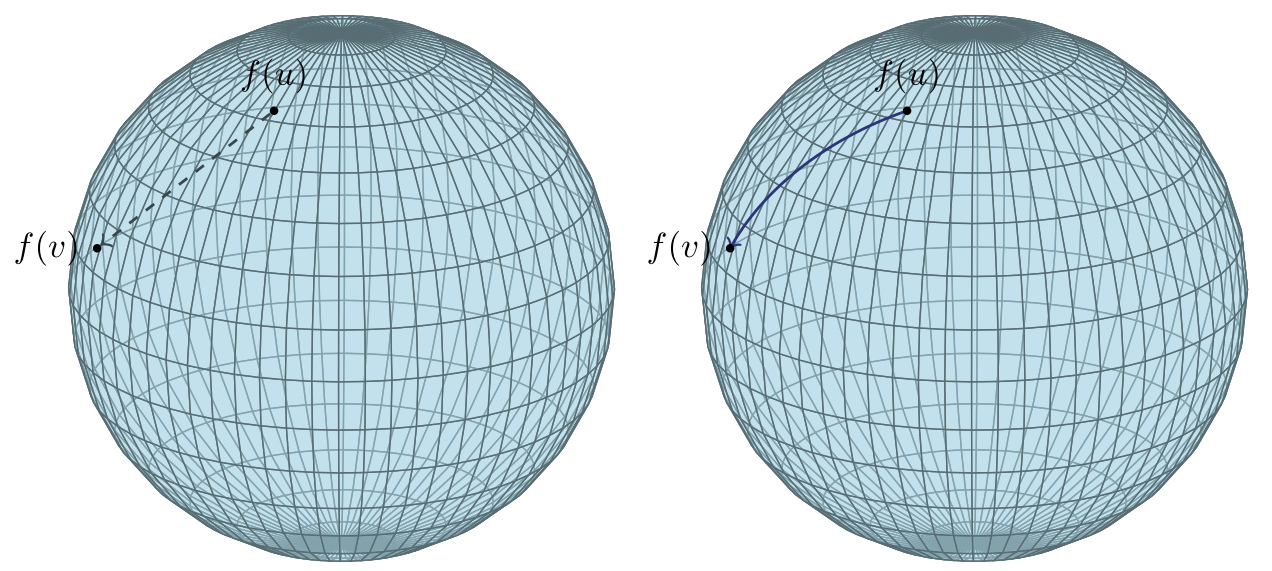
\includegraphics[width=\textwidth]{../\string_build/html/\string_images/mannigfaltigkeit.png}
\caption{Visualisierung zweier unterschiedlicher Abstandsbegriffe für Punkte auf der Kugeloberfläche \(\mathbb{S}^2\).}\label{\detokenize{vektoranalysis/diffformen:fig-kugel}}\end{figure}

\par
Aus dieser Anschauung wird klar, dass unser bisheriges Konzept von Differenzierbarkeit im Mehrdimensionalen aus dem \href{https://fau-ammn.github.io/MathDataScience2/ableitungen/ableitungen.html}{MP 2 Skript} nicht ausreicht, um auf diesem Objekt geeignet Funktionen abzuleiten.
Da man in vielen Bereichen der Physik und der Mathematik nicht nur auf offenen Teilmengen des \(\R^n\) ableiten möchte, benötigen wir ein analoges Prinzip für topologische Räume \(\M := (\M, \tau)\).

\par
\textbf{Wie können wir den Ableitungsbegriff auf topologische Räume übertragen?}

\par
Die grundlegende Idee ist es, den topologischen Raum \(\M\) lokal mit einer Teilmenge des \(\R^n\) zu identifizieren.
Für eine beliebige offene Teilmenge \(U\subset \M\) betrachten wir also eine Abbildung
\begin{align*}
\phi:U\rightarrow \R^n.
\end{align*}
\par
Wir wollen fordern, dass es sich bei \(\phi\) um eine \emph{injektive Abbildung} handelt, so dass eine inverse Abbildung \(\phi^{-1}\) existiert.
Diese Umkehrabbildung müssen wir jedoch auf das Bild \(\phi(U) \subset \R^n\) einschränken, damit sie wohldefiniert ist.
Damit erhalten wir eine \emph{lokale Bijektion} \(\phi^{-1}:\phi(U)\rightarrow U\).

\par
Betrachten wir nun eine Funktion \(f \colon \M \rightarrow \R^m\), die Punkte des topologischen Raumes auf Punkte des \(\R^m\) abbildet.
Wenn wir diese Funktion differenzieren möchten, so sehen wir ein, dass die Verknüpfung
\begin{align*}
f \circ \phi^{-1} : \phi(U) \subset \R^n \to \R^m
\end{align*}
\par
es uns erlaubt, das Problem der Ableitung in topologischen Räumen auf das Konzept der mehrdimensionalen Differentiation im \(\R^n\) zurückzuführen.


\subsubsection{Karten und Atlanten auf topologischen Räumen}
\label{\detokenize{vektoranalysis/diffformen:karten-und-atlanten-auf-topologischen-raumen}}
\par
Um den Ableitungsbegriff auf topologischen Räumen \(\M\) formal definieren zu können, benötigen wir zusätzlich zur Bijektivität der Abbildung \(\phi \colon U \rightarrow \phi(U) \subset \R^n\) die Bedingung, dass für jede Teilmenge \(U \subset \M\) gilt,
\begin{align*}
\phi(U)\text{ ist offen} \ \Leftrightarrow \ U \text{ ist offen}.
\end{align*}
\par
Diese Forderung bedeutet, dass offene Teilmengen in \(U \subset \M\) gerade mit offenen Teilmengen in \(\phi(U) \subset \R^n\) identifiziert werden.
Wir wollen im Folgenden beide Implikationsrichtungen diskutieren.

\par
1. \(\phi(U)\) ist offen \(\Rightarrow U \) ist offen.

\par
Diese Implikation ist äquivalent zur Forderung, dass Urbilder offener Mengen selbst wieder offen sind.
Mit \cref{vektoranalysis/diffformen:def:stetigkeitTopologie} bedeutet dies wiederum, dass die Abbildung \(\phi\) stetig ist.

\par
2. \(\phi(U)\) ist offen \(\Leftarrow U \) ist offen.

\par
Analog zur obigen Überlegung sehen wir ein, dass diese Bedingung gerade aussagt, dass \(\phi^{-1}\) stetig ist.
Diese Forderung ist nicht immer trivialerweise erfüllt.

\par
Das folgende Beispiel zeigt, dass es tatsächlich stetige bijektive Abbildung \(\phi\) gibt, für die gilt, dass die Umkehrabbildung \(\phi^{-1}\) \emph{nicht stetig} ist.
\begin{example}{}{vektoranalysis/diffformen:ex:nonho}



\par
Wir betrachten in diesem Beispiel die Funktion
\begin{align*}
\phi:[0,2\pi)&\to\R^2,\\
t &\mapsto \phi(t):= (\cos(t), \sin(t)).
\end{align*}
\par
Wir erkennen, dass \(\phi([0,2\pi)) = \S^1\) gerade der Einheitskreis ist, und dass \(\phi:[0,2\pi)\to\S^1\) bijektiv und stetig ist.
Allerdings stellen wir fest, dass die Umkehrabbildung nicht stetig ist.
Sei dazu \((x_i)_{i\in\N}\) eine Folge von Punkten auf dem Einheitskreis \(\S^1\), deren \(y\) Koordinate negativ ist und die gegen den Punkt \(x = (1,0) \in \S^1\) konvergieren, d.h.,
\begin{align*}
\lim_{i\rightarrow\infty} x_i =: x = (1,0) \in \S^1.
\end{align*}
\par
Betrachten wir jedoch den Grenzwert der Folge von Funktionswerten \((\phi^{-1}(x_i))_{i\in I}\), so sehen wir, dass
\begin{align*}
\lim_{i\to\infty} \phi^{-1} (x_i) = 2\pi \neq 0 = \phi^{-1}(x)
\end{align*}
\par
und somit ist \(\phi^{-1}\) offensichtlich nicht stetig.
\end{example}

\begin{figure}[htbp]
\centering


\noindent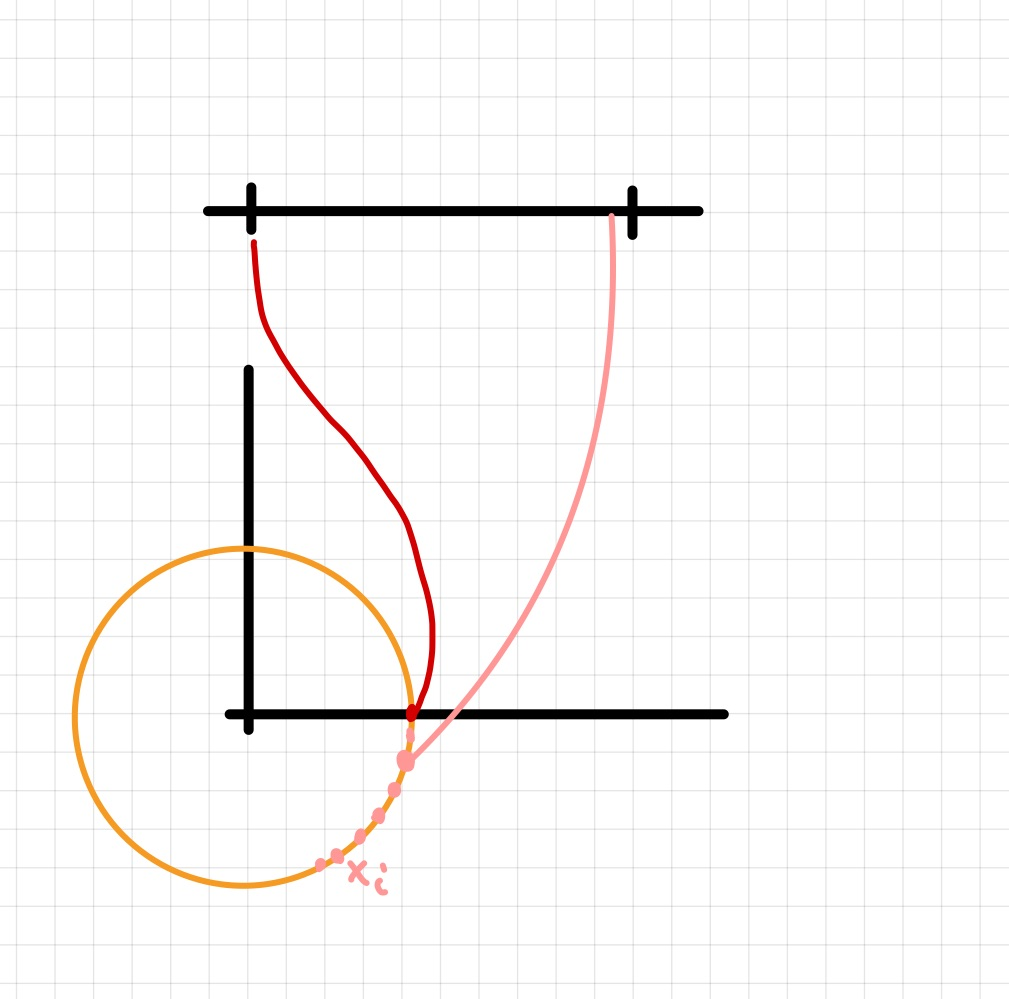
\includegraphics[width=\textwidth]{../\string_build/html/\string_images/nonhomöo.jpg}
\caption{Visualisierung einer unstetigen Umkehrabbildung für das \cref{vektoranalysis/diffformen:ex:nonho} }\label{\detokenize{vektoranalysis/diffformen:fig-nonh}}\end{figure}

\par
Insgesamt fordern wir also, dass \(\phi:U\rightarrow\phi(U)\) bijektiv ist und zusätzlich, dass sowohl \(\phi\) als auch die Umkehrabbildung \(\phi^-1\) stetig sind.
Eine solche Abbildung definiert man unter dem Begriff \emph{Homöomorphismus}.
\begin{definition}{}{vektoranalysis/diffformen:definition-5}



\par
Seien \(X\) und \(Y\) topologische Räume.
Dann nennen wir eine Abbildung \(f \colon X \rightarrow Y\) einen \textbf{Homöomorphismus}, wenn sie folgende Eigenschaften erfüllt:
\begin{enumerate}

\item {} 
\par
\(f\) ist bijektiv

\item {} 
\par
\(f\) ist stetig

\item {} 
\par
die Umkehrfunktion \(f^{-1}\) ist ebenfalls stetig.

\end{enumerate}
\end{definition}

\par
Speziell im Kontext von Mannigfaltigkeiten \(\M\), als Spezialfall topologischer Räume (wie wir noch sehen werden), nennt man eine offene Menge zusammen mit einem Homöomorphismus eine \textbf{Karte} auf \(\M\).
\begin{definition}{}{vektoranalysis/diffformen:definition-6}



\par
Es sei \(\M\) ein topologischer Raum und \(U\subset\M\) eine offene Menge.
Sei außerdem \(\phi:U\rightarrow \phi(U)\subset \R^n\) ein Homöomorphismus.
Dann heißt das Tupel \((U,\phi)\) \textbf{Karte} auf \(\M\).
\end{definition}

\par
Um einen Ableitungsbegriff für Funktionen \(f:\M\to\R^m\) über eine Karte \((U,\phi)\) und der Verknüpfung \(f\circ \phi^{-1}\) zu definieren benötigen wir noch ein zusätzliches Konzept.
Denn in der Situation, dass \((V,\psi)\) eine zweite Karte ist, deren offene Menge \(V\) einen nichtleeren Schnitt mit der offenen Menge \(U\) hat, d.h., \(U\cap V \neq \emptyset\), erhalten wir genau auf dem Schnitt dieser Mengen zwei unterschiedliche Parametrisierungen,
\begin{align*}
f\circ \phi^{-1} = (f\circ\psi^{-1})\circ(\psi\circ \phi^{-1}),\\
f\circ \psi^{-1} = (f\circ\phi^{-1})\circ(\phi\circ \psi^{-1}).
\end{align*}
\par
Um von einer Karte zur nächsten Karte zu kommen benötigen wir eine geeignete Abbildung.
\begin{definition}{}{vektoranalysis/diffformen:definition-7}



\par
Es sei \(\M\) ein topologischer Raum und es seien \((U,\phi)\) und \((V,\psi)\) zwei Karten auf \(\M\) mit nicht leerem Schnitt, d.h., \(U\cap V\neq \emptyset\).
Dann nennt man die Abbildung
\begin{align*}
\psi\circ\phi^{-1}: \phi(U\cap V)\rightarrow \psi(U\cap V)
\end{align*}
\par
einen \textbf{Kartenwechsel} von \((U,\phi)\) nach \((V,\psi)\).
\end{definition}

\begin{figure}[htbp]
\centering


\noindent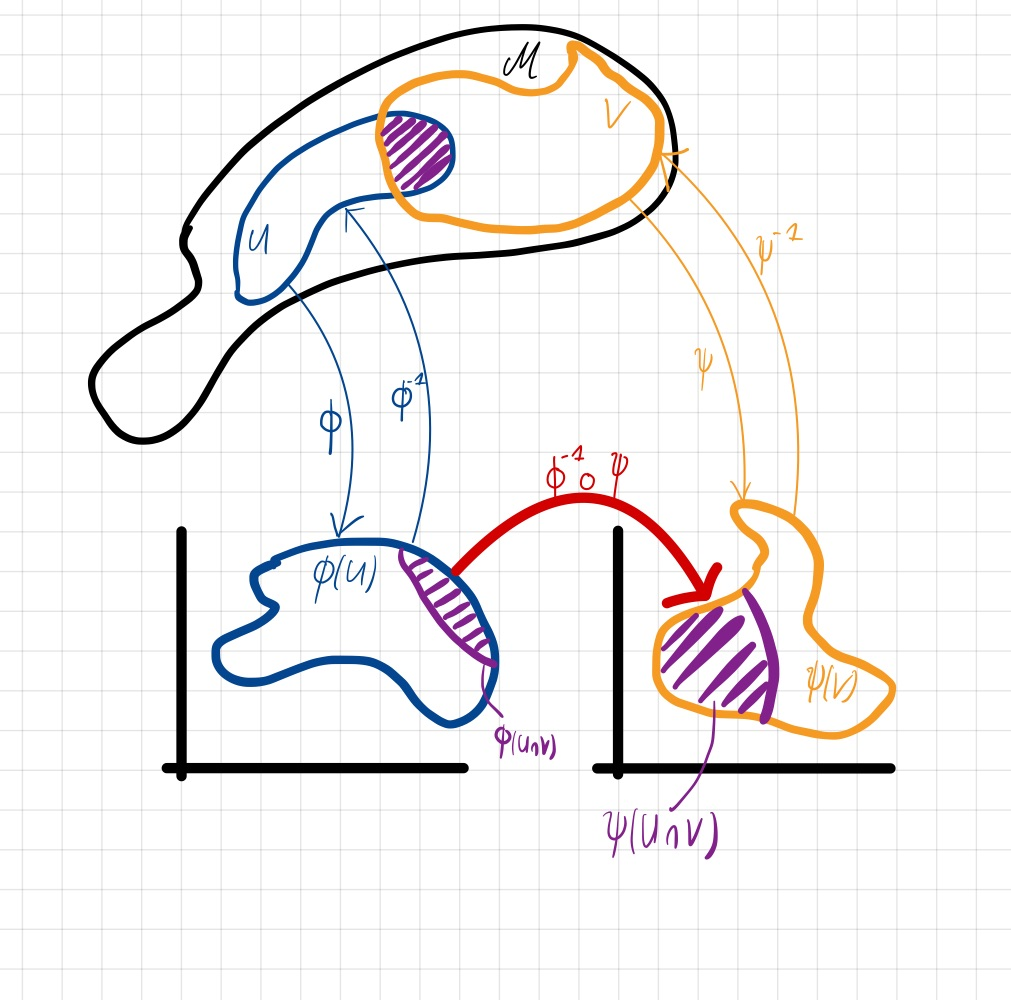
\includegraphics[width=\textwidth]{../\string_build/html/\string_images/chartchange.jpg}
\caption{Kartenwechsel.}\label{\detokenize{vektoranalysis/diffformen:fig-chartchange}}\end{figure}

\par
Wir erkennen also, dass Umparametrisierungen der Form \(\psi\circ \phi^{-1}\) entscheidend sind, um von einer lokalen Identifikation des topologischen Raums zur nächsten zu gelangen.
Wäre nun der Kartenwechsel \(\psi\circ \phi^{-1}\) und respektive \(\phi\circ \psi^{-1}\) differenzierbar, so könnte man die jeweiligen Ableitungen leicht durch die Kettenregel ineinander umrechnen.
Allerdings existieren durchaus Beispiele, in denen sowohl \(f\circ\phi^{-1}\) als auch \(f\circ\psi^{-1}\) differenzierbar sind, aber der Kartenwechsel \(\psi\circ\phi^{-1}\) nicht.
Deshalb führt man zusätzlich noch den folgenden Begriff ein.
\begin{definition}{}{vektoranalysis/diffformen:definition-8}



\par
Es sei \(\M\) ein topologischer Raum.
Eine Familie von Karten \(\mathcal{A} = (U_i,\phi_i)_{i\in I}\) indiziert durch die Indexmenge \(I\) heißt \textbf{Atlas}, falls die Vereinigung aller offenen Mengen eine Überdeckung des topologischen Raums darstellt, d.h., es gilt
\begin{align*}
\M = \bigcup_{i\in I} U_i.
\end{align*}
\par
Wir nennen einen Atlas \(k\) mal \textbf{differenzierbar} oder von der Klasse \(C^k\), falls jeder Kartenwechsel \(\phi_i\circ\phi_j^{-1}, i,j\in I\) \(k\) mal stetig differenzierbar ist.
\end{definition}

\par
Die Begriffe \emph{Karte} und \emph{Atlas} stammen in der Tat aus mathematischen Überlegungen in der Kartographie.
Man kann Teile der Erdoberfläche mit einer Karte auf eine Ebene \(\R^2\) abbilden.
Nähert man sich dem Rand einer Karte, so möchte man zu einer anderen Karte wechseln, die das angrenzende Gebiet darstellt.

\par
So kann eine Mannigfaltigkeit durch einen vollständigen Satz von Karten vollständig beschrieben werden; man braucht dabei Regeln, wie sich beim Kartenwechsel die Karten überlappen.


\subsubsection{Differenzierbare Mannigfaltigkeiten}
\label{\detokenize{vektoranalysis/diffformen:differenzierbare-mannigfaltigkeiten}}
\par
Für einen topologischen Raum \(\M\) können mehrere Atlanten \(\mathcal{A}\) existieren, weshalb es sinnvoll ist Äquivalenzklassen von Atlanten zu betrachten.
\begin{definition}{}{vektoranalysis/diffformen:definition-9}



\par
Für einen Index \(k\in \N \cup \{\infty\}\) heißen zwei differenzierbare Atlanten \(\mathcal{A}_1, \mathcal{A}_2\) der Klasse \(C^k\) \textbf{\(k\) äquivalent}, falls ihre Vereinigung \(\mathcal{A}_1\cup \mathcal{A}_2\) wieder ein Atlas der Klasse \(C^k\) ist.
Dies bedeutet insbesondere, dass die Kartenwechsel durch die Vereinigung der beiden Atlanten weiterhin \(k\) mal stetig differenzierbar bleiben.
In diesem Fall notieren wir \(\mathcal{A}_1\sim_k \mathcal{A}_2\).
Die Äquivalenzklasse \([\mathcal{A}]_{\sim_k}\) nennt man eine \textbf{\(C^k\) differenzierbare Struktur}.
\end{definition}

\begin{emphBox}{}{}

\par
\href{https://de.wikipedia.org/wiki/Felix\_Hausdorff}{Felix Hausdorff} (geboren am 8. November 1868 in Breslau; gestorben am 26. Januar 1942 in Bonn) war ein deutscher Mathematiker.
\end{emphBox}

\par
Bisher haben wir \(\M\) als allgemeinen topologischen Raum betrachtet.
In vielen Anwendungen benötigt man aber weitere nützliche Eigenschaften des Raumes.
Insbesondere wenn man \href{https://de.wikipedia.org/wiki/Testfunktion}{glatte Testfunktionen} und \href{https://en.wikipedia.org/wiki/Partition\_of\_unity}{die Zerlegung der Eins} benutzen möchte braucht man folgende zwei zusätzliche Eigenschaften.

\par
Wir definieren zunächst die Eigenschaft eines Hausdorff Raums.
\begin{definition}{}{vektoranalysis/diffformen:definition-10}



\par
Ein topologischer Raum \(\M\) heißt \textbf{Hausdorff Raum}, falls für je zwei unterschiedliche Punkte \(x,y\in \M, x\neq y\) offene Umgebungen \(U(x), U(y) \subset \M\) existieren, welche disjunkt sind, d.h., \(U(x)\cap U(y) = \emptyset\).
Man nennt \(\M\) dann auch einen \textbf{separierten Raum}.
\end{definition}

\par
Als zweite nützliche Eigenschaft fordern wir, dass unser topologischer Raum \(\M\) das zweite Abzählbarkeitsaxiom erfüllen soll.
\begin{definition}{}{vektoranalysis/diffformen:definition-11}



\par
Ein toplogischer Raum \((\M, \tau)\) erfüllt das \textbf{zweite Abzählbarkeitsaxiom}, falls \emph{abzählbar} viele offene Mengen \((V_i)_{i\in\N} \in \tau\) existieren, so dass für jeden Punkt \(x\in \M\) und jede offene Umgebung \(U(x) \in \tau\) von \(x\) mindestens ein Index \(k\in\N\) existiert mit \(V_k \subset U(x)\).
Man nennt \((\M, \tau)\) dann auch \textbf{zweitabzählbar}.
\end{definition}

\par
Diese zwei Bedingung wirken zunächst abstrakt.
Glücklicherweise werden sie jedoch von vielen üblichen topologischen Räumen erfüllt, wie zum Beispiel dem Euklidischen Raum \(\R^n\).
\begin{remark}{}{vektoranalysis/diffformen:remark-12}



\par
Falls der Begriff eines zweitabzählbaren Hausdorff Raums zu unhandlich erscheint, kann man für die meisten Anwendungen in der Physik auch einfach \textbf{metrische Räume} betrachten, die diese beiden Eigenschaften implizieren.
\end{remark}

\par
Nun haben wir alle nötigen Voraussetzungen geschaffen um den Begriff einer Mannigfaltigkeit formal einzuführen.
\begin{definition}{}{vektoranalysis/diffformen:definition-13}



\par
Es sei \(\M\) ein zweitabzählbarer Hausdorff Raum und für \(k\in\N\cup \{\infty\}\) sei \([\mathcal{A}]_{\sim_k}\) eine \(C^k\) differenzierbare Struktur.
Dann nennen wir \((\M,[\mathcal{A}]_{\sim_k})\) eine \(k\) \textbf{mal differenzierbare Mannigfaltigkeit}.
Für den Spezialfall \(k=\infty\) sprechen wir auch von einer \textbf{glatten Mannigfaltigkeit}.

\par
Falls alle Karten auf \(\M\) nach \(\R^n\) abbilden, so nennt man die Mannigfaltigkeit \emph{\(n\) dimensional}.
\end{definition}

\par
Ähnlich wie bei topologischen Räumen spricht man in den meisten Fällen nur von der Mannigfaltigkeit \(\M\); die differenzierbare Struktur \([\mathcal{A}]_{\sim_k}\) wird dabei implizit vorausgesetzt.

\par
Basierend auf einer differenzierbaren Mannigfaltigkeit \(\M\) können wir nun differenzierbare Funktionen auf \(\M\) definieren.
\begin{definition}{}{vektoranalysis/diffformen:definition-14}



\par
Sei \(\M\) eine \(k\) mal differenzierbare Mannigfaltigkeit \(\mathcal{A}\) ein Atlas auf \(\M\).
Dann nennen wir eine Abbildung \(f:\M\to\R^m\) \textbf{\(k\) mal differenzierbar}, falls für jeden Punkt \(x\in\M\) eine differenzierbare Karte \((U(x),\phi)\in\mathcal{A}\) existiert, so dass \(f\circ\phi^{-1} \in C^k(\phi(U(x)); \R^m)\).
Insbesondere schreiben wir in diesem Fall \(f\in C^k(\M; \R^m)\).
\end{definition}

\par
In vielen Anwendungen beschränkt man sich nur auf \emph{glatte Mannigfaltigkeiten} und \emph{glatte Funktionen} in \(C^\infty(\M; \R^m)\).
Wir werden im Folgenden der Einfachheit halber auch dazu übergehen.
\begin{lemma}{}{vektoranalysis/diffformen:lemma-15}



\par
Es sei \(\M\) eine glatte Mannigfaltigkeit.
Dann ist \(C^\infty(\M; \R^m)\) ein reeller Vektorraum mit den Verknüpfungen
\begin{align*}
(\lambda \cdot f)(x) := \lambda\cdot f(x)\text{ für } f\in C^\infty(\M; \R^m), \lambda\in\R,\\
(f + g)(x) := f(x) + g(x)\quad\text{ für } f,g\in C^\infty(\M; \R^m).
\end{align*}\end{lemma}

\begin{proof}
 In der Hausaufgabe zu zeigen.
\end{proof}

\par
Die Eigenschaft der Differenzierbarkeit einer Funktion auf einer Mannigfaltigkeit ist kartenunabhängig, wie folgendes Lemma feststellt.
\begin{lemma}{}{vektoranalysis/diffformen:lem:differenzierbarkeitKartenunabhaengig}



\par
Es sei \(\M\) eine glatte Mannigfaltigkeit und \(\mathcal{A}\) ein Atlas auf \(\M\).
Außerdem sei \(f:\M \to \R^m\) eine Funktion, \((U,\phi)\in \mathcal{A}\) eine Karte und \(x \in U\) ein Punkt in der offenen Menge \(U\).
Ist \(f\circ\phi^{-1}\) differenzierbar in \(x\), so ist \(f\circ\psi^{-1}\) auch differenzierbar in \(x\) für jede Karte \((V,\psi) \in \mathcal{A}\) mit \(x\in V\).
\end{lemma}

\begin{proof}
 In der Hausaufgabe zu zeigen.
\end{proof}


\subsubsection{Tangentialräume an Mannigfaltigkeiten}
\label{\detokenize{vektoranalysis/diffformen:tangentialraume-an-mannigfaltigkeiten}}
\par
Aus dem Kapitel \cref{odestability/ruhelagen:s-linearisierung-ruhelage}  ist bereits das Konzept der \emph{Linearisierung} bekannt.
Anschaulich gesprochen haben wir eine differenzierbare Funktion \(f\) durch ihre Linearisierung ersetzt um ein einfacheres Problem zu erhalten.
Dieses Konzept soll nun auf glatte Mannigfaltigkeiten übertragen werden.

\par
Wir haben bereits erkannt, wie wir den Begriff der Differenzierbarkeit einer Funktion auf einer Mannigfaltigkeit definieren.
Und obwohl die Frage nach der Differenzierbarkeit einer Funktion nach \cref{vektoranalysis/diffformen:lem:differenzierbarkeitKartenunabhaengig} kartenunabhängig ist, so stellt sich heraus, dass der tatsächliche \emph{Wert der Ableitung} einer Verknüpfung \(f \circ\phi^{-1}\) noch immer von der konkreten Wahl des Homöomorphismus \(\phi\) abhängt.
Um auch hier die gewünschte Kartenunabhängigkeit zu erreichen, brauchen wir einen anderen Begriff der Differenzierbarkeit.
Hierbei wird uns der sogenannte \textbf{Tangentialraum} helfen.
Man kann ihn als eine Linearisierung der Mannigfaltigkeit \(\M\) an einem Punkt \(p\in\M\) interpretieren.

\par
Das folgende Beispiel erklärt anschaulich den Tangentialraum an eine Mannigfaltigkeit.
\begin{example}{}{vektoranalysis/diffformen:example-17}



\par
Wir betrachten zunächst den Einheitskreis \(\M = \mathbb{S}^1\) und den Punkt \(p = (1, 0)^T \in \mathbb{S}^1\).
Der Tangentialraum \(T_p\M\) an \(\M\) im Punkt \(p\) ist der eindimensionale Unterraum
\begin{align*}
T_p\M = \lbrace \lambda \cdot (0, 1)^T : \lambda \in \R \rbrace \subset \R^2.
\end{align*}\end{example}

\par
Es gibt in der Literatur zwei verschiedene, jedoch äquivalente Arten den Tangentialraum zu definieren.
\begin{itemize}
\item {} 
\par
\textbf{Geometrischer Tangentialraum}: Bei diesem Ansatz wählt man eine geometrisch Anschauung und definiert den Tangentialraum durch Richtungsvektoren, die am Punkt \(p\in\M\) anliegen.
Der Vorteil dieser Definition ist es, dass sie intuitiv und geometrisch anschaulich ist.

\item {} 
\par
\textbf{Algebraische Defnition}: Bei diesem Ansatz führt man den Tangentialraum mittels spezieller linearer Abbildungen, genannt Derivationen, zurück.
Man verliert hierbei zwar die geometrische Anschauung, allerdings ist das Konzept relativ einfach zu formulieren und hilft die Sachverhalte auf algebraische Zusammenhänge zurückzuführen.

\end{itemize}

\par
In der Praxis (und in vielen Mathematikbüchern) werden beide Definitionen nebeneinander verwendet und die jeweilige Interpretation geht dann aus dem Kontext hervor.
Da sich die beiden Konzepte somit schlecht voneinander trennen lassen werden wir im Folgenden den geometrischen Tangentialraum \(T^{\text{geo}}_p\M\) und den algebraischen Tangentialraum \(T^{\text{alg}}_p\M\) explizit einführen und anschließend eine Isomorphie
\begin{align*}
T^{\text{geo}}_p\M\cong T^{\text{alg}}_p\M
\end{align*}
\par
zwischen den beiden Tangentialräumen zeigen.

\begin{emphBox}{}{}
\par
In der Literatur wird diese explizite Unterscheidung oft nicht vorgenommen.
Stattdessen wird der Tangentialraum einfach nur \(T_p\M\) genannt.
Elemente dieses Raums sind dann je nach Kontext geometrisch oder algebraisch zu interpretieren.
\end{emphBox}


\paragraph{Geometrische Definition}
\label{\detokenize{vektoranalysis/diffformen:geometrische-definition}}
\par
Von der Differentiation im Mehrdimensionalen ist bereits das Konzept der \textbf{Richtungsableitung} bekannt (siehe Kapitel 6.2.2 in \cite{Ten21}).
Hierbei betrachtet man für eine Funktion \(F:\R^n\to\R\) den Strahl \(\gamma(t):= x + t\cdot v\), wobei \(x,v\in\R^n\) und den Grenzwert
\begin{align*}
\lim_{t\to 0} \frac{F(\gamma(t)) - F(\gamma(0))}{t} = \frac{F(x + t\cdot v) - F(x))}{t}.
\end{align*}
\par
Wir werden dieses Konzept nun auf glatte \(n\) dimensionale Mannigfaltigkeiten \(\M\) verallgemeinern, indem wir anstatt von Strahlen differenzierbare \emph{Kurven} auf der Mannigfaltigkeit betrachten.
\begin{definition}{}{vektoranalysis/diffformen:definition-18}



\par
Sei \(\M\) eine glatte Mannigfaltigkeit und sei
\begin{align*}
\gamma \colon (-1,1) \rightarrow \M
\end{align*}
\par
eine Kurve auf der Mannigfaltigkeit \(\M\).
Wir nennen \(\gamma\) \textbf{differenzierbar} im Punkt \(0\in(-1,1)\), falls die Kurve \emph{stetig} ist und falls eine Karte \((U,\phi)\) von \(\M\) existiert, so dass für genügend kleines \(\varepsilon\) auch \(\gamma((-\varepsilon,\varepsilon))\subset U\) gilt und die Verknüpfung
\begin{align*}
\phi \circ \gamma:(-\varepsilon,\varepsilon)\to\R^n
\end{align*}
\par
differenzierbar in \(0\) ist .
\end{definition}

\par
Wir werden im Folgenden ausschließlich die Ableitung der Kurve im Punkt \(t=0\) betrachten und sprechen deshalb verkürzt einfach nur von \emph{differenzierbaren} Kurven.
Zusätzlich sei zu bemerken, dass die obige Definition \textbf{nicht} von der Wahl der Karte abhängt.
\begin{example}{}{vektoranalysis/diffformen:example-19}



\par
Es sei \(\M=\S^2\) die Einheitssphäre und \(f:\M\to\R\) beschreibe eine Wärmeverteilung auf deren Oberfläche.
Betrachtet man nun die Bahn eines Partikels auf der Oberfläche beschrieben durch die Kurve \(\gamma:(-t, t)\to \M\) so erhalten wir eine eindimensionale Abbildung
\begin{align*}
f\circ\gamma:(-t,t)\to \R,
\end{align*}
\par
die zu jedem Zeitpunkt die Temperatur des Ortes, an dem sich der Partikel befindet, beschreibt.
\end{example}

\begin{figure}[htbp]
\centering


\noindent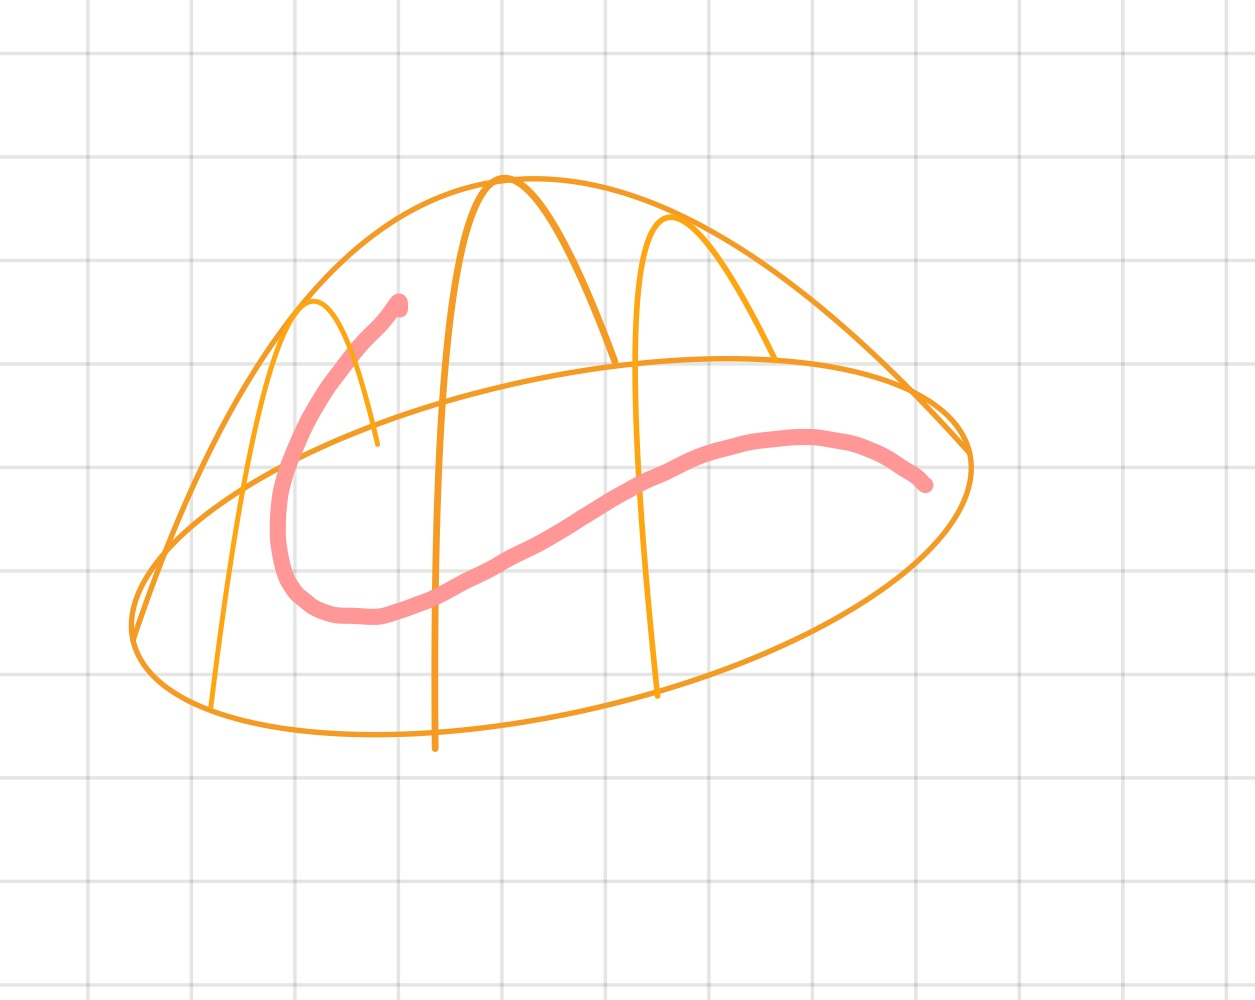
\includegraphics[width=\textwidth]{../\string_build/html/\string_images/velocity.jpg}
\caption{Visualisierung einer Kurve auf der oberen Hälfte der Einheitssphäre im \(\R^3\).}\label{\detokenize{vektoranalysis/diffformen:fig-velocity}}\end{figure}

\par
Mit Hilfe von differenzierbaren Kurven auf Mannigfaltigkeiten können wir im Folgenden die Richtungsableitung an einer Mannigfaltigkeit definieren.
\begin{definition}{}{vektoranalysis/diffformen:def:direcdiv}



\par
Es sei \(\M\) eine glatte Mannigfaltigkeit, \(\gamma:(-1,1)\to\M\) eine differenzierbare Kurve mit \(\gamma(0)=p\in\M\) und \(f \in C^\infty(\M)\) eine glatte Funktion.
Dann nennen wir die Abbildung
\begin{align*}
D_\gamma : C^\infty(\M) &\to \R\\
f &\mapsto D_\gamma(f):=\frac{d}{dt}(f\circ \gamma)\big\rvert_{t=0}
\end{align*}
\par
\textbf{Richtungsableitung} von \(f\) durch \(\gamma\) im Punkt \(p\).
\end{definition}

\par
Betrachten wir nun eine differenzierbare Kurve \(\gamma \colon (-1, 1) \rightarrow \M\) mit \(\gamma(0)=p \in \M\) und eine glatte Funktion \(f \in \C^\infty(\M)\) definiert auf einer glatten Mannigfaltigkeit \(\M\).
Dann können wir die Richtungsableitung \(D_\gamma(f)\) mit Hilfe der \textbf{Kettenregel für die Differentiation} darstellen als
\begin{align*}
D_\gamma(f) = \frac{d}{dt}(f\circ \gamma)\big\rvert_{t=0} = \frac{d}{dt}\big( (f\circ \phi^{-1}) (\phi \circ \gamma) \big)\rvert_{t=0} = 
\big(D(f\circ \phi^{-1})\big)(\phi(p))\cdot \frac{d}{dt}(\phi \circ \gamma)\rvert_{t=0}
\end{align*}
\par
und für eine weitere differenzierbare Kurve \(\eta \colon (-1, 1) \rightarrow \M\) mit \(\eta(0)=p\) erhalten wir analog
\begin{align*}
D_\eta(f) = \frac{d}{dt}(f\circ \eta)\big\rvert_{t=0} = 
\big(D(f\circ \phi^{-1})\big)(\phi(p))\cdot \frac{d}{dt}(\phi \circ \eta)\rvert_{t=0}.
\end{align*}
\par
Wir erkennen also, dass der Wert der Richtungsableitung in der Tat von der Kurve \(\gamma\) abhängt.
Dies führt auf einen natürlichen Äquivalenzbegriff von Kurven, wie die folgende Bemerkung beschreibt.
\begin{remark}{}{vektoranalysis/diffformen:rem:tang}



\par
Es sei \(\M\) eine glatte \(n\) dimensionale Mannigfaltigkeit, \(p\in\M\) ein Punkt auf der Mannigfaltigkeit und \((U,\phi)\) eine Karte von \(\M\), für die gilt, dass \(p\in U\) ist.
Für zwei differenzierbare Kurven \(\gamma, \eta:(-1,1) \to U\) mit \(\gamma(0) = \eta(0) = p\) ist die Relation
\begin{align*}
\gamma \sim_p \eta
\qquad \Leftrightarrow \qquad
\frac{d}{dt}(\phi \circ \gamma)\rvert_{t=0} = \frac{d}{dt}(\phi \circ \eta)\rvert_{t=0}\in \R^n
\end{align*}
\par
eine Äquivalenzrelation (siehe Kapitel 2.1.1 in \cite{Bur20}).
Insbesondere ist die Äquivalenzklasse unabhängig von der Wahl des Homöomorphismus \(\phi\).
\end{remark}

\par
Mittels der oben beschriebenen Äquivalenzrelation sind wir in der Lage den Begriff der \emph{Tangentialvektoren} und des \emph{Tangentialraums} zu definieren.
\begin{definition}{}{vektoranalysis/diffformen:definition-22}



\par
Es sei \(\M\) eine glatte \(n\) dimensionale Mannigfaltigkeit, \(p\in\M\) ein Punkt auf der Mannigfaltigkeit und \((U,\phi)\) eine Karte von \(\M\), für die gilt, dass \(p\in U\) ist.

\par
Die Äquivalenzklasse \(\gamma^\prime(0):=[\gamma]_{\sim_p}\) wird als \textbf{geometrischer Tangentialvektor} an \(\M\) im Punkt \(p\) bezeichnet.
Der Raum der (geometrischen) Tangentialvektoren
\begin{align*}
T_p^{\text{geo}}\M := \{\gamma^\prime(0): \gamma\text{ ist differenzierbare Kurve mit }\gamma(0)=p\}
\end{align*}
\par
heißt \textbf{geometrischer Tangentialraum} der Mannigfaltigkeit \(\M\) am Punkt \(p \in \M\).
\end{definition}

\par
Der Tangentialraum induziert sogar eine Vektorraumstruktur wie folgende Bemerkung festhält.
\begin{remark}{}{vektoranalysis/diffformen:remark-23}



\par
Es sei \(\M\) eine glatte \(n\) dimensionale Mannigfaltigkeit, \(p\in\M\) ein Punkt auf der Mannigfaltigkeit und \((U,\phi)\) eine Karte von \(\M\), für die gilt, dass \(p\in U\) ist.
Sei außerdem \(\gamma \colon (-1,1) \rightarrow \M\) eine differenzierbare Kurve auf \(\M\) mit \(\gamma(0) = p\).
Wir definieren nun die folgende Bijektion auf dem Tangentialraum
\begin{align*}
d\phi\rvert_p \colon T^{\text{geo}}_p\M &\rightarrow \R^n,\\
[\gamma]_{\sim_p} &\mapsto d\phi\rvert_p (\gamma^\prime(0)) := (\phi \circ \gamma)^\prime (0).
\end{align*}
\par
Basierend auf dieser Abbildung lassen sich die folgenden Operationen für den Punkt \(p \in \M\) definieren
\begin{align*}
\gamma^\prime(0) +_{p} \eta^\prime(0) \ &:= \
(d\phi\rvert_p)^{-1}\big[d\phi\rvert_p(\gamma^\prime(0)) + d\phi\rvert_p(\eta^\prime(0))\big]\\
\lambda \cdot_p \gamma^\prime(0) \ &:= \ (d\phi\rvert_p)^{-1} (\lambda \cdot d\phi\rvert_p(\gamma^\prime(0))
\end{align*}
\par
Insgesamt ergibt somit das Tripel \((T_p^{\text{geo}}\M, +_p, \cdot_p)\) einen reellen Vektorraum.
Man bemerke, dass die oben definierten Abbildungen erneut \textbf{unabhängig} von der Wahl des Homöomorphismus \(\phi\) sind.
\end{remark}


\paragraph{Algebraische Definition}
\label{\detokenize{vektoranalysis/diffformen:algebraische-definition}}
\par
Alternativ zur geometrischen Herleitung lässt sich der Tangentialraum auch algebraisch definieren über sogenannte \emph{Derivationen}.
Hierbei beschreiben wir Tangentialvektoren nun nicht mehr als Kurven, sondern als spezielle Funktionale, welche durch ihre Wirkung auf \(C^\infty(\M)\) charakterisiert sind.
Die Motivation hierbei soll die Richtungsableitung aus \cref{vektoranalysis/diffformen:def:direcdiv} sein und speziell die im folgenden Lemma beschriebenen Eigenschaften.
\begin{lemma}{}{vektoranalysis/diffformen:lemma-24}



\par
Es sei \(\M\) eine glatte Mannigfaltigkeit und \(p\in\M\) und \(\gamma:[-1,1]\to\M\) eine glatte Kurve durch \(p\).
Dann gilt für die Richtungsableitung \(D_\gamma:C^\infty(\M)\to\R\),
\begin{itemize}
\item {} 
\par
\(D_\gamma\in (C^\infty(\M))^\ast\),

\item {} 
\par
Für \(f,g\in C^\infty(\M)\) gilt: \(\ D_\gamma(fg) = D_\gamma(f) g(p) + f(p) D_\gamma(g)\).

\end{itemize}
\end{lemma}

\begin{proof}
 Siehe Übung.
\end{proof}

\par
Die zweite Eigenschaft wird auch \textbf{Produktregel} oder \textbf{Leibnizregel} genannt.
Wir wollen nun im Folgenden nicht nur Richtungsableitungen betrachten, sondern allgemeine Funktionale, die diese Eigenschaft erfüllen.
\begin{definition}{}{vektoranalysis/diffformen:definition-25}



\par
Es sei \(\M\) eine glatte Mannigfaltigkeit und \(p\in\M\) ein Punkt der Mannigfaltigkeit.
Wir nennen eine lineare Abbildung \(D: C^\infty(\M) \to \R\) eine \textbf{Derivation} an \(p\), falls sie die folgende Produktregel erfüllt,
\begin{align*}
D(fg) = D(f) g(p) + f(p) D(g).
\end{align*}
\par
Der Raum der Derivationen an \(p\)
\begin{align*}
T^{\text{alg}}_p\M := \{D\in C^\infty(\M)^\ast: D\text{ ist Derivation an }p\}
\end{align*}
\par
wird als \textbf{algebraischer Tangentialraum} bezeichnet.
\end{definition}

\par
Über die Menge der Derivation erhalten wir auf natürliche Art einen Vektorraum da per Definition
\begin{align*}
T^{\text{alg}}_p\M \subset (C^\infty(\M))^\ast
\end{align*}
\par
gilt.
Somit erbt der algebraischer Tangentialraum die Vektorraumoperationen von \(C^\infty(\M)^\ast\) und es muss lediglich nachgeprüft werden, dass diese Teilmenge noch immer ein Vektorraum, also inbesondere abgeschlossen ist.
\begin{lemma}{}{vektoranalysis/diffformen:lemma-26}



\par
Es sei \(\M\) eine glatte Mannigfaltigkeit und \(p\in\M\) ein Punkt der Mannigfaltigkeit.
Dann ist \(T^{\text{alg}}_p\M\) ein reeller Vektorraum.
\end{lemma}

\begin{proof}
 Siehe Übung.
\end{proof}

\par
Wie der Name schon erkennen lässt haben Derivationen gewisse Eigenschaften, die von der Ableitungsoperation bekannt sind.
So bildet zum Beispiel jede Derivation konstante Funktionen auf \(0\) ab, wie das folgende Lemma zeigt.
\begin{lemma}{}{vektoranalysis/diffformen:lem:constder}



\par
Es sei \(\M\) eine glatte Mannigfaltigkeit und \(p\in\M\) ein Punkt der Mannigfaltigkeit.
Außerdem sei \(f\in C^\infty(\M)\) eine konstante Funktion, d.h., es existiert eine Konstante \(c\in\R\), so dass
\begin{align*}
f(q) = c\quad\forall q\in\M.
\end{align*}
\par
Dann gilt schon \(D(f)=0\) für alle Derivationen \(D\in T^{\text{alg}}_p\M\).
\end{lemma}

\begin{proof}
 Es sei \(D\in T^{\text{alg}}_p\M\) eine beliebige Derivation an den Punkt \(p \in \M\).
Wir betrachten zunächst die konstante Einsfunktion
\begin{align*}
g:\M &\to \R\\
q &\mapsto g(x) := 1.
\end{align*}
\par
Dann gilt mit der Produktregel für Derivationen
\begin{align*}
D(g) = D(g\cdot g) = D(g)\,g(p) + g(p)\, D(g) = 2\,D(g)
\end{align*}
\par
und somit muss schon \(D(g) = 0\) gelten.
Wir können die konstante Funktion \(f\) nun darstellen als \(f= c\,g\) und unter Ausnutzung der Linearität von \(D\) erhalten wir schon
\begin{align*}
D(f) = D(c\,g) = c\,D(g) = 0.
\end{align*}\end{proof}

\par
Wir haben nun zwei verschiedene Arten gesehen den Tangentialraum einzuführen.
Tatsächlich sind diese Definitionen äquivalent in dem Sinn, dass ein Isomorphismus zwischen dem geometrischen und algebraischen Tangentialraum existiert.
\begin{theorem}{(Isomorphie zwischen alg. und geom. Tangentialraum)}{vektoranalysis/diffformen:theorem-28}



\par
Es sei \(\M\) eine glatte Mannigfaltigkeit und \(p\in\M\) ein Punkt der Mannigfaltigkeit.
Dann gilt die folgende Isomorphie
\begin{align*}
T^{\text{geom}}_p\M \ \cong \ T^{\text{alg}}_p\M.
\end{align*}\end{theorem}

\begin{proof}
 Siehe z.B. Kapitel 2.3 in \cite{Janich03}.
\end{proof}


\paragraph{Basis des algebraische Tangentialraums}
\label{\detokenize{vektoranalysis/diffformen:basis-des-algebraische-tangentialraums}}\label{\detokenize{vektoranalysis/diffformen:sec-tpbasis}}
\par
Wir wollen in diesem Abschnitt eine Basis des algebraischen Tangentialraums konstruieren.
Im Euklidischen Raum können wir auf natürliche Art die Koordinatenrichtungen als Kurven wählen, also Funktionen der Form
\begin{align*}
t \mapsto t e_i
\end{align*}
\par
für \(i=1,\ldots,n\), wobei \(e_i\) den \(i\) ten Einheitsvektor in \(\R^n\) bezeichnet.
Um diese Idee auf Mannigfaltigkeiten zu übertragen wählen wir eine Karte \(\varphi:\M\to\R^n\), wobei man hier auch von
\begin{align*}
\varphi = (\varphi_1,\ldots,\varphi_n) =: (x^1,\ldots,x^n)
\end{align*}
\par
als einem \textbf{lokalen Koordinatensystem} spricht.
Wir erhalten somit Kurven
\begin{align*}
\gamma_{x^i}(t):= \varphi^{-1}(\varphi(p) + t e_i)
\end{align*}
\par
und mithilfe der Richtungsableitung aus \cref{vektoranalysis/diffformen:def:direcdiv} die Derivationen
\begin{align*}
\partial_{x^i}^p: C^\infty(\M) &\to \R\\
f &\mapsto \partial_{x^i}^p(f) := \frac{d}{dt} (f\circ \gamma_{x^i}(t)).
\end{align*}\begin{definition}{}{vektoranalysis/diffformen:definition-29}



\par
Sei \(\M\) eine glatte \(n\) dimensionale Mannigfaltigkeit für \(n\in\N\) und sei \(f \in C^\infty(\M)\) eine glatte Funktion.
Dann bezeichnen wir die Derivationen
\begin{align*}
\partial_{x^i}^p (f) := \frac{d}{dt} (f\circ \gamma_{x^i}(t)), \quad i=1,\ldots,n
\end{align*}
\par
als \textbf{partielle Derivationen} von \(f\) im Punkt \(p \in \M\).
\end{definition}

\par
Wir interpretieren also im Folgenden das Symbol \(\partial_{x^{i}}^p\) als Derivation an \(p\in\M\), d.h., insbesondere als lineare Abbildung von \(C^\infty(\M)\) nach \(\R\).
Diese partiellen Derivationen folgen der Intuition, dass die partielle Ableitung in eine Richtung auch nur Änderungen in diese Richtung respektiert.
Wir formalisieren diese Anschauung in folgendem Lemma.
\begin{lemma}{}{vektoranalysis/diffformen:lem:partderkron}



\par
Es sei \(\M\) eine glatte Mannigfaltigkeit, \(p\in\M\) ein Punkt der Mannigfaltigkeit und \((U,\varphi)\) sei eine Karte mit \(p\in U\).
Dann gilt für die partielle Derivation
\begin{align*}
\partial_{x^i}^p(\varphi_j) = \delta_{ij},
\end{align*}
\par
wobei \(\delta_ij\) das \emph{Kronecker Delta} bezeichnet.
\end{lemma}

\begin{proof}
 Wir betrachten zunächst die Funktion \(\varphi_j \circ \gamma_{x^i}\) und erhalten für \(t\in [-1,1]\)
\begin{align*}
\varphi_j \circ \gamma_{x^i}(t)
&= \varphi_j \circ \varphi^{-1}(\varphi(p) + t e_i)\\
&= (\varphi(p) + t e_i)_j\\ 
&=
\begin{cases}
\varphi(p) + t e_i &\text{ für } i=j,\\
\varphi_j(p)&\text{ sonst}.
\end{cases}
\end{align*}
\par
Somit gilt schon für die partielle Derivation
\begin{align*}
\partial_{x^i}^p(\varphi_j)=
\frac{d}{dt} (\varphi_j \circ \gamma_{x^i}(t)) = 
\begin{cases}
1&\text{ für } i=j,\\
0&\text{ sonst}.
\end{cases}
\end{align*}\end{proof}

\par
Das folgende Hauptresultat dieses Abschnitts erlaubt es uns beliebige Derivationen mithilfe der partiellen Derivationen darzustellen, da diese eine Basis des algebraischen Tangentialraums bilden.
\begin{theorem}{}{vektoranalysis/diffformen:thm:tanbasis}



\par
Es sei \(\M\) eine \(n\) dimensionale glatte Mannigfaltigkeit.
Dann bildet die Menge
\begin{align*}
\{\partial_{x^1}^p,\ldots,\partial_{x^n}^p\}
\end{align*}
\par
eine Basis des algebraischen Vektorraums \(T^{\text{alg}}_p\).
Insbesondere gilt
\begin{align*}
\dim(T^{\text{alg}}_p)=\dim(T^{\text{geom}}_p)=n
\end{align*}\end{theorem}

\begin{proof}
 Es sei \((U,\varphi)\) eine Karte der Mannigfaltigkeit \(\M\) und wir nehmen ohne Beschränkung der Allgemeinheit an, dass \(\varphi(p)=0 \in \R^n\) gilt, was stets durch eine entsprechende Translation des Koordinatensystems erreicht werden kann.
Zusätzlich wählen wir einen Radius \(r>0\) klein genug, so dass \(B_r(0) \subset \varphi(U)\) gilt und betrachten als Karte \(\tilde{\varphi} := \varphi\rvert_{\tilde{U}}\), d.h., die Einschränkung von \(\varphi\) auf \(\tilde{U}:= \varphi^{-1}(B_r(0))\).
Wir können die Karte \(\tilde{\varphi}\) wegen der Kartenunabhängigkeit des Tangentialraums und der Tatsache, dass \((\tilde{U},\tilde{\varphi})\) auch eine Karte der Mannigfaltigkeit \(\M\) mit \(p\in \tilde{U}\) ist, betrachten.
Da das Bild von \(\tilde{\varphi}\) nun der gesamte Ball \(B_r(0) \subset \R^n\) ist, können wir nun Strecken von \(0\) zu einem beliebigen Punkt in \(B_r(0)\) betrachten, welche selbst ganz im Bild von \(\tilde{\varphi}\) enthalten sind.

\par
Sei nun \(f\in C^\infty(\M)\) eine beliebige glatte Funktion.
Dann definieren wir die Funktion \(g:= f\circ \tilde{\varphi}^{-1}\) für die insbesondere \(g\in C^\infty(\R^n)\) gilt.
Für einen beliebigen Punkt \(q\in\tilde{U}\) erhalten wir einen Richtungsvektor \(z:=\tilde{\varphi}(q)\in B_r(0)\) und können somit die Einschränkung von \(g\) auf die eindimensionale Strecke zwischen \(0\) und \(z\) in \(\R^n\) betrachten, d.h.,
\begin{align*}
\tilde{g}:[0,1] &\to\R\\
t&\mapsto g(t\cdot z).
\end{align*}
\par
Hierbei sieht man erneut ein, dass \(\tilde{g}\in C^\infty([0,1])\) gilt.
Dies bedeutet insbesondere, dass wir den \emph{Hauptsatz der Differential  und Integralrechnung} (vgl. Theorem 5.3 in \cite{Ten21}) anwenden können und somit erhalten wir
\begin{align*}
\tilde{g}(1) = \tilde{g}(0) + \int_{0}^1 \tilde{g}^\prime(t)\,\mathrm{d}t.
\end{align*}
\par
Wir berechnen die Ableitung im Integral als Richtungsableitung und erhalten,
\begin{align*}
\int_{0}^1 \tilde{g}^\prime(t) \,\mathrm{d}t
=\int_{0}^1 \langle \nabla g (t\cdot z), z \rangle \,\mathrm{d}t
=\sum_{i=1}^{n} \int_{0}^1  \partial_i g (t\cdot z) \cdot z_i \,\mathrm{d}t.
\end{align*}
\par
Da per Definition
\begin{align*}
\tilde{g}(1) = g(z)=f(q)
\end{align*}
\par
und
\begin{align*}
\tilde{g}(0) = g(0) = g(\varphi(p))=f(p)
\end{align*}
\par
gilt, folgt daraus
\begin{align*}
f(q) = 
f(p) + 
\sum_{i=1}^{n} \varphi_i(q)\ \cdot \underbrace{\int_{0}^1  \partial_i (f\circ \varphi^{-1})(t\cdot \varphi(q)) \, \mathrm{d}t}_{:=F_i(q)}.
\end{align*}
\par
An diesem Punkt bemerken wir, dass \(f\circ \varphi^{-1} \in C^\infty(\R^n)\) eine klassisch differenzierbare Funktion ist, wobei \(f\) eine glatte Funktion auf der Mannigfaltigkeit \(\M\) darstellt.
Wenden wir nun die \(j\) te partielle Derivation auf \(f\) an, erhalten wir unter Ausnutzung der Linearität der Abbildung \(\partial_{x^j}^p\)
\begin{align*}
\partial_{x^j}^p (f) = 
\underbrace{\partial_{x^j}^p (f(p))}_{=0} + 
\sum_{i=1}^{n} \partial_{x^j}^p(\varphi_i \cdot F_i) = 
\sum_{i=1}^{n} \partial_{x^j}^p(\varphi_i \cdot F_i)
\end{align*}
\par
wobei wir \cref{vektoranalysis/diffformen:lem:constder} und die Tatsache, dass \(\varphi_i, F_i\in C^\infty(\M)\) gilt, benutzt haben.
Weiterhin gilt wegen der Leibnizregel
\begin{align*}
\partial_{x^j}^p(\varphi_i \cdot F_i(q)) = 
\underbrace{\partial_{x^j}^p(\varphi)}_{=\delta_{ij}} F_i(p)+ \underbrace{\varphi_i(p)}_{=0} \partial_{x^j}^p(F_i),
\end{align*}
\par
wobei wir \cref{vektoranalysis/diffformen:lem:partderkron} und \(\varphi(p)=0\) verwendet haben.
Somit folgt schon
\begin{align*}
\partial_{x^j}^p (f) = F_j(p)
\end{align*}
\par
und damit insbesondere
\begin{align*}
f = f(p) + \sum_{i=1}^{n} \varphi_i \partial_{x^i}^p(f).
\end{align*}
\par
Dies bedeutet aber schon, dass die partiellen Derivationen ein \textbf{Erzeugendensystem} des algebraischen Tangentialraums bilden, denn sei \(D\in T^{\text{alg}}_p\) eine beliebige Derivation, dann gilt
\begin{align*}
D(f) = \underbrace{D(f(p))}_{=0} + \sum_{i=1}^n D(\varphi_i) \partial_{x^i}^p(f).
\end{align*}
\par
Dies bedeutet, dass jede Derivation \(D\) über eine Linearkombination aus partiellen Derivationen dargestellt werden kann, wobei die Koeffizienten durch \(D(\varphi_i)\) gegeben sind.

\par
Es bleibt die Eindeutigkeit der Darstellung zu zeigen.
Seien dazu Koeffizienten \(\alpha_i \in \R, i=1,\ldots,n\) gegeben, so dass für jede Funktion \(f\in C^\infty(\M)\) gilt
\begin{align*}
D:= \sum_{i=1}^n \alpha_i \partial_{x^i}^p(f) = 0.
\end{align*}
\par
Durch erneute Anwendung von \cref{vektoranalysis/diffformen:lem:partderkron} erhalten wir aber, dass
\begin{align*}
0 = D(\varphi_j) = \alpha_j\end{align*}
\par
für alle \(j=1,\ldots,n\) und somit haben wir die \textbf{lineare Unabhängigkeit} bewiesen.

\par
Insgesamt bilden also die partiellen Deriviationen eine Basis des algebraischen Tangentialraums und es gilt
\begin{align*}
\dim(T^{\text{alg}}_p)=\dim(T^{\text{geom}}_p)=n.
\end{align*}\end{proof}


\paragraph{Kotangentialraum}
\label{\detokenize{vektoranalysis/diffformen:kotangentialraum}}
\par
Da wir den Tangentialraum \(T^{\text{alg}}_p\) als Vektorraum identifiziert haben, können wir auch dessen algebraischen Dualraum in der folgenden Definition betrachten.
\begin{definition}{}{vektoranalysis/diffformen:definition-32}



\par
Es sei \(\M\) eine glatte Mannigfaltigkeit.
Dann bezeichnen wir mit
\begin{align*}
T_p^\ast\M:= (T_p^{\text{alg}}\M)^\ast
\end{align*}
\par
den algebraischen Dualraum des Tangentialraums, welcher häufig \textbf{Kotangentialraum} genannt wird.
\end{definition}
\begin{remark}{}{vektoranalysis/diffformen:remark-33}



\par
Ein Element \(\delta\in T_p^\ast\M\) ist also eine lineare Abbildung
\begin{align*}
\delta: T_p^{\text{alg}}\M \to \R,
\end{align*}
\par
die eine Derivation \(D\in C^\infty(\M)^\ast\) auf eine reelle Zahl \(\delta(D)\in\R\) abbildet.
\end{remark}

\par
Die folgende Definition beschreibt ein wichtiges Element des Kotangentialraums.
\begin{definition}{}{vektoranalysis/diffformen:definition-34}



\par
Sei \(f\in\C^\infty(\M)\) eine beliebige glatte Funktion auf einer Mannigfaltigkeit \(\M\).
Dann bezeichnen wir das Element \(\mathrm{d}f_p \in T_p^\ast\M\) mit
\begin{align*}
\mathrm{d}f_p: T_p^{\text{alg}}\M &\to\R\\
D_p &\mapsto \mathrm{d}f_p(D):= D_p(f).
\end{align*}
\par
als \textbf{totales Differential} der Funktion \(f\) im Punkt \(p \in \M\).
\end{definition}

\par
Insbesondere können wir das totale Differential \(df\) mit einer glatten Funktion aus \(C^\infty(M)\) identifizieren, was den Zusammenhang von \(T^\ast_p \M\) als Bidualraum von \(C^\infty(\M)\) unterstreicht.

\par
Die Basis von \(T^\ast_p\) wird kanonisch als duale Basis (siehe \cref{vektoranalysis/multilinear:lem:dualeBasis}  gewählt.
Jeder Vektor \(v\in T_p^{\text{alg}}\M\) hat somit eine eindeutige Darstellung
\begin{align*}
v = \sum_{i=1}^n \alpha_i \partial_{x^i}.
\end{align*}
\par
Wir wählen nun Abbildungen \(\mathrm{d}x^i\in T^\ast_p\M, i=1,\ldots,n\) gerade so, dass
\begin{align*}
\mathrm{d}x^i(v) = \alpha_i
\end{align*}
\par
gilt.
Das folgende Lemma zeigt, dass es sich hierbei um eine Basis von \(T^\ast_p\M\) handelt.
\begin{lemma}{}{vektoranalysis/diffformen:lemma-35}



\par
Es sei \(\M\) eine glatte Mannigfaltigkeit und \(p\in\M\).
Dann ist die Menge
\begin{align*}
\{\mathrm{d}x^1,\ldots, \mathrm{d}x^n\}
\end{align*}
\par
eine Basis von \(T_p^\ast\M\).
\end{lemma}

\begin{proof}
 Die Aussage folgt direkt aus \cref{vektoranalysis/multilinear:lem:dualeBasis} 
\end{proof}


\subsubsection{Tangentialbündel}
\label{\detokenize{vektoranalysis/diffformen:tangentialbundel}}
\begin{emphBox}{}{}{Note:}
\par
Im Folgenden bezeichne \(T_p\M\in\{T^{\text{alg}}_p\M, T^{\text{geom}}_p\M \}\) entweder den \emph{algebraischen} oder den \emph{geometrischen Tangentialraum}.
Die konkrete Wahl wird an den entsprechenden Stellen (wenn nötig) spezifiziert.
\end{emphBox}

\par
Bisher haben wir für eine \(n\) dimensionale glatte Mannigfaltigkeit \(\M\) für jeden einzelnen Punkt \(p\in\M\) den zugehörigen Tangentialraum \(T_p\M\) betrachtet, welcher wiederum wegen \cref{vektoranalysis/diffformen:thm:tanbasis} isomorph zum \(\R^n\) ist.
Wir interessieren uns jetzt dafür, wie sich Tangentialräume für verschiedene Punkte \(p,q\in \M\) in Beziehung setzen lassen.
Darüber hinaus wollen wir eine globale Struktur definieren welche alle Tangentialräume (d.h. für jedes \(p\in\M\)) zusammenfasst.

\par
In diesem Kontext spricht man von der Mannigfaltigkeit häufig als dem \textbf{Basisraum} \(B=\M\), da die Punkte \(p \in \M\), welche die Vektorräume erzeugen, aus diesem Raum entnommen werden.
Ein erster Ansatz für eine globale Struktur ist die Vereinigung
\begin{align*}
\bigcup_{p\in\M} T_p\M.
\end{align*}
\par
Wir wollen diese Idee im folgenden Beispiel veranschaulichen.
\begin{example}{}{vektoranalysis/diffformen:ex:tangentialS1}



\par
Sei als zu Grunde liegende Mannigfaltigkeit der Einheitskreis \(\M = \mathbb{S}^1\subset\R^2\) gegeben.
Wir wählen als Repräsentanten für jeden Punkt
\begin{align*}
p=(\cos(\alpha), \sin(\alpha))\in\M, \quad \alpha\in (0,2\pi) \setminus \{\pi\}
\end{align*}
\par
die Kurve
\begin{align*}
\gamma_p(t) := p - t \cdot\big(1, \frac{\cos(\alpha)}{\sin(\alpha)}\big),
\end{align*}
\par
und somit erhalten wir anschaulich die in \hyperref[\detokenize{vektoranalysis/diffformen:fig-bundlea}]{Fig.\@ \ref{\detokenize{vektoranalysis/diffformen:fig-bundlea}}} für einige Punkte visualisierte Menge.

\par
Es fällt auf, dass sich zwar einzelne Kurven schneiden können, jedoch die Kurven selbst und die assoziierten Vektorräume nicht gleich sind.
Um diese Tatsache zu verdeutlichen ist es praktisch die \emph{disjunkte Vereinigung}
\begin{align*}
\bigsqcup_{p\in\M} T_p\M := \bigcup_{p\in\M} \{p\} \times T_p\M \cong \bigcup_{p\in\M} \{p\} \times \R
\end{align*}
\par
zu betrachten.
Für den Einheitskreis erhalten wir durch die Isomorphie \(T_p\M \cong \R\) so den Zylinder in \hyperref[\detokenize{vektoranalysis/diffformen:fig-bundleb}]{Fig.\@ \ref{\detokenize{vektoranalysis/diffformen:fig-bundleb}}}.
\end{example}

\begin{figure}[htbp]
\centering


\noindent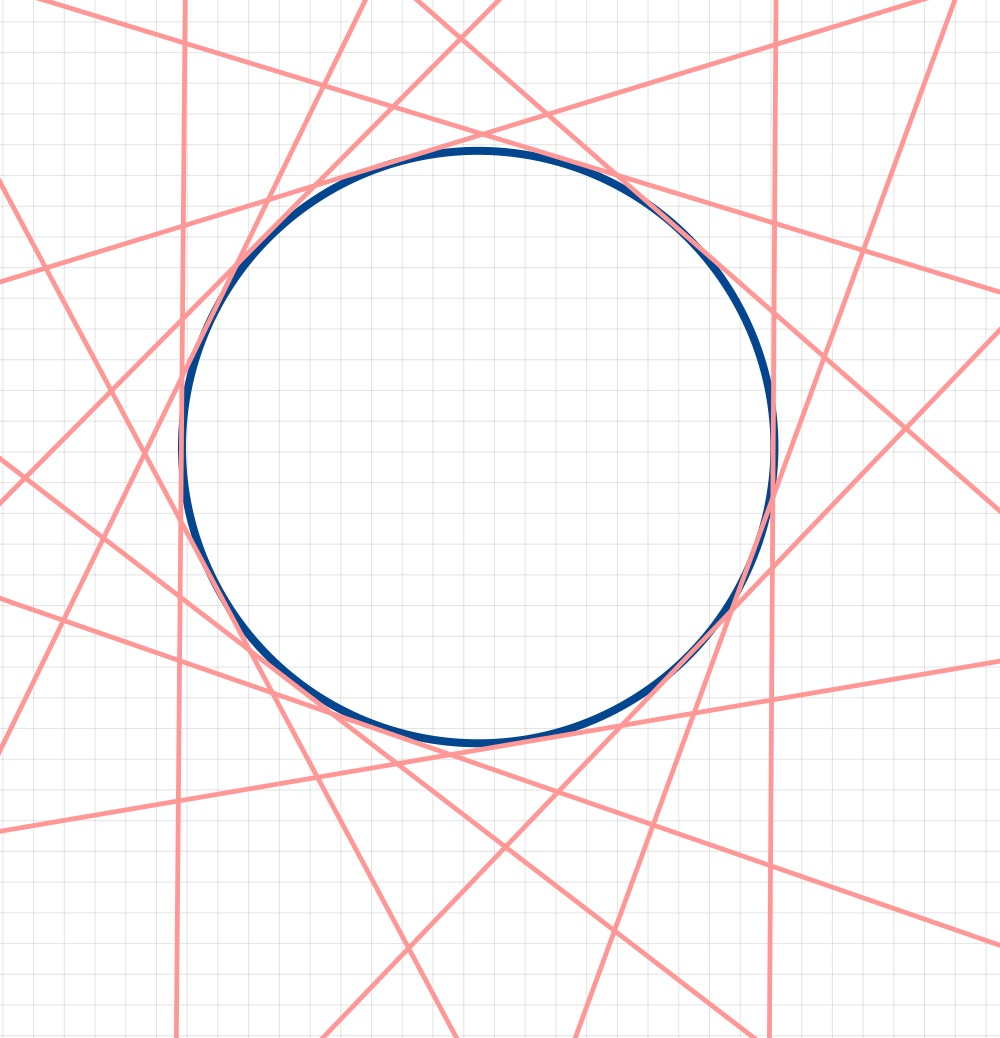
\includegraphics[width=\textwidth]{../\string_build/html/\string_images/bundlea.jpg}
\caption{Visualisierung der Tangentialräume einiger Punkte am Einheitskreises.}\label{\detokenize{vektoranalysis/diffformen:fig-bundlea}}\end{figure}

\begin{figure}[htbp]
\centering


\noindent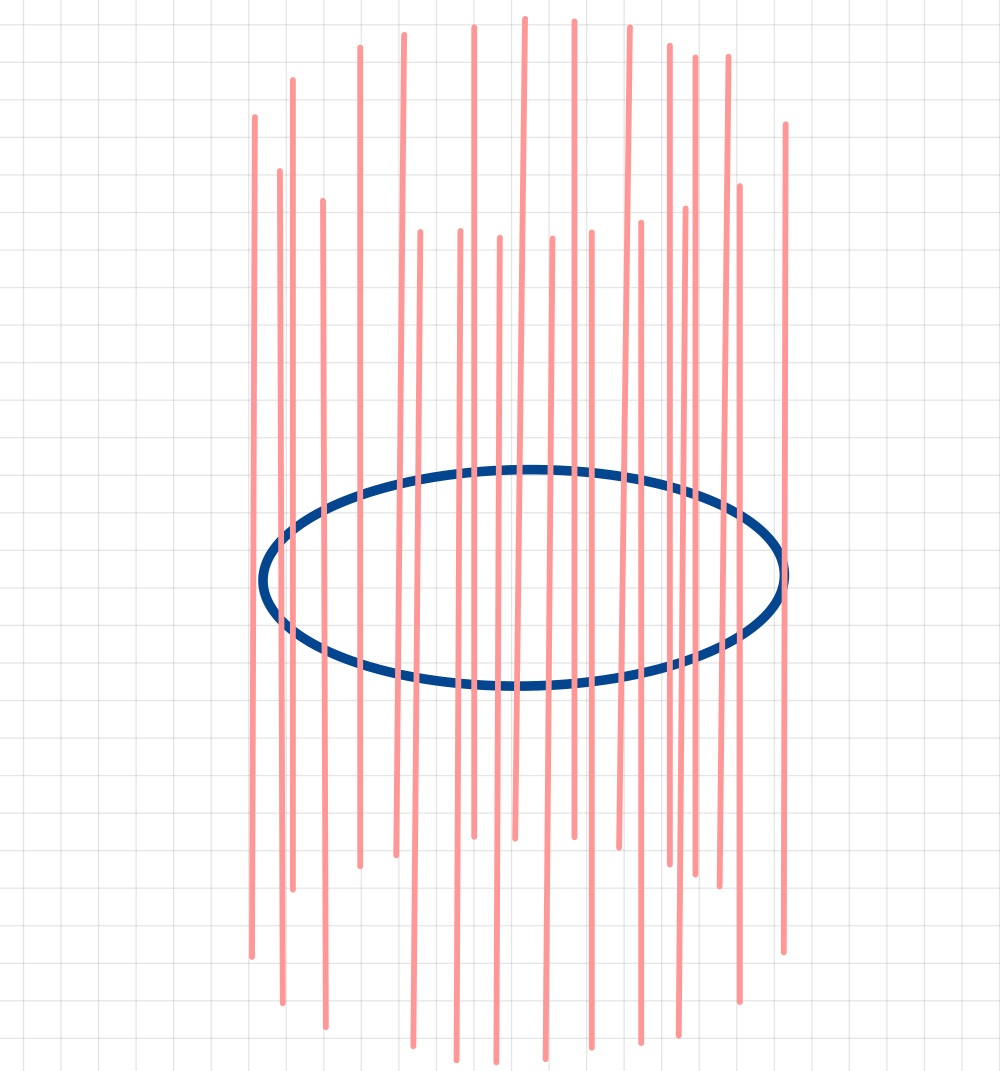
\includegraphics[width=\textwidth]{../\string_build/html/\string_images/bundleb.jpg}
\caption{Visualisierung der disjunkt vereinigten Tangentialräume einiger Punkte am Einheitskreises.}\label{\detokenize{vektoranalysis/diffformen:fig-bundleb}}\end{figure}

\par
Wir wollen diese globale Struktur der disjunkten Vereinigung formal definieren.
\begin{definition}{}{vektoranalysis/diffformen:definition-37}



\par
Es sei \(\M\) eine glatte Mannigfaltigkeit.
Dann heißt die Menge
\begin{align*}
T\M := \bigsqcup_{p\in\M}  T_p\M = \bigcup_{p\in\M} \{p\} \times T_p\M
\end{align*}
\par
zusammen mit der Projektion
\begin{align*}
\pi:T\M &\to \M\\
\{p\}\times T_p\M &\mapsto p
\end{align*}
\par
das \textbf{Tangentialbündel} von \(\M\).
\end{definition}

\par
Insbesondere erkennen wir, dass wir mit Hilfe der Projektion \(\pi\) jedem Element des Tangentialbündels eindeutig den zu Grunde liegenden Punkt \(p\in\M\) zuordnen können, der den entsprechenden Tangentialraum erzeugt hat.

\par
Im Folgenden wollen wir uns zwei Beispiele für Tangentialbündel an Mannigfaltigkeiten ansehen.
\begin{example}{}{vektoranalysis/diffformen:example-38}





\par
1. Sei \(\M=\R^n\).
Dann ist das Tangentialbündel gerade gegeben durch
\begin{align*}
T\M = \R^n\times\R^n = \R^{2n}.
\end{align*}


\par
2. Wie bereits in \cref{vektoranalysis/diffformen:ex:tangentialS1} gesehen erhalten wir für \(\M=\mathbb{S}^1\) als Tangentialbündel den unendlich hohen Zylinder
\begin{align*}
T\M = \mathbb{S}^1\times \R.
\end{align*}\end{example}

\par
In den bisher betrachten Beispielen haben wir als Tangentialbündel jeweils eine Menge der Form \(\M\times \R^n\) erhalten.
Dies ist jedoch nicht immer der Fall wie wir sehen werden.
Tatsächlich bilden Tangentialbündel von dieser Form eine spezielle Unterklasse.
\begin{definition}{}{vektoranalysis/diffformen:definition-39}



\par
Sei \(\M\) eine glatte \(n\) dimesnionale Mannigfaltigkeit.
Das Tangentialbündel \(T\M\) heißt \textbf{trivial}, falls gilt
\begin{align*}
T\M\cong \M\times\R^n.
\end{align*}
\par
In diesem Fall nennt man die Mannigfaltigkeit \(\M\) auch \textbf{parallelisierbar}.
\end{definition}
\begin{remark}{}{vektoranalysis/diffformen:remark-40}



\par
Es lässt sich zeigen, dass \(\mathbb{S}^1, \mathbb{S}^3,\mathbb{S}^7\) die \emph{einzigen} paralleslisierbaren Sphären sind (siehe \cite{Lee03}).
Die Tatsache, dass \(\mathbb{S}^2\) nicht parallelisierbar ist wird beim Satz vom gekämmten Igel in {prf:ref broken reference}\{TODO\} erneut auftauchen.
\end{remark}

\par
Wir wollen uns nun mit der Frage beschäftigen, wie sich die Tangentialräume für unterschiedliche Punkte \(p,q\in B\) des Basisraums zueinander verhalten, insbesondere wenn \(p\) und \(q\) nahe beieinander liegen.
Hierbei hilft es das abstraktee Konzept eines \textbf{Vektorbündels} zu betrachten.
\begin{definition}{}{vektoranalysis/diffformen:definition-41}



\par
Es seien \(\M\) (der sog. Basisraum) und \(E\) (der sog. Totalraum) zwei glatte Mannigfaltigkeiten und \(\pi:E\to \M\) sei glatt und bijektiv. Weiterhin gelte
Außerdem sei \(\pi:E\to \M\) eine glatte und bijektive Abbildung.
Weiterhin gelte
\begin{itemize}
\item {} 
\par
für jeden Punkt \(p\in \M\) sei die sogenannte \textbf{Faser} \(E_p:= \pi^{-1}(p)\) ein \(n\) dimensionaler Vektorraum,

\item {} 
\par
für jeden Punkt \(p\in \M\) existiere eine offene Umgebung \(U\subset \M\) und ein Diffeomorphimus \(\Psi: \pi^{-1}(U)\to U\times\R^n\), so dass für alle \(x\in U\) gilt

\end{itemize}
\begin{align*}
\text{pr}_U(\Psi(x)) &= \pi(x)\quad\forall x\in \pi^{-1}(U)\\
\Psi\rvert_{E_q}&: \pi^{-1}(q) \to \{q\}\times \R^n \text{ ist ein Isomorphismus, für alle }q\in U.
\end{align*}
\par
Dann heißt \((E,\M,\pi)\) \textbf{Vektorbündel} vom Rang \(n\).
Hierbei bezeichnet \(\text{pr}_U(q, z):= q\) die Projektion auf die \(U\) Komponente eines Vektors \((q,z)\in U\times\R^n\).
\end{definition}
\begin{remark}{}{vektoranalysis/diffformen:remark-42}



\par
Anstatt das Vektorbündel \((E,\M,\pi)\) als Tripel aufzuschreiben, ist es üblich von einem Bündel \(E\overset{\pi}{\to}\M\) oder sogar \(E\to\M\) zu sprechen.
Die Abbildung \(\pi\) wird im zweiten Fall nur \emph{implizit} vorausgesetzt.
\end{remark}

\par
Die Funktion \(\Psi\) nennt man in diesem Kontext \textbf{lokale Trivialisierung}, denn sie erlaubt es uns den Totalraum \(E\) lokal als Produktraum darzustellen.
Analog zum Tangentialbündel nennen wir ein Vektorbündel \textbf{trivial}, falls eine Trivialsierung \(\Psi:E\to \M\times\R^n\) existiert, so dass gilt
\begin{align*}
E \cong \M\times\R^n.
\end{align*}\begin{example}{}{vektoranalysis/diffformen:example-43}



\par
Möbius Band.
\end{example}

\par
Wir wollen nun zeigen, dass das Tangentialbündel ein Vektorbündel ist.
Dazu benötigen wir zunächst die Hilfsaussage des folgenden Lemmas, dass das Tangentialbündel \(T\M\) selbst eine glatte Mannigfaltigkeit ist.
\begin{lemma}{}{vektoranalysis/diffformen:lem:tanman}



\par
Es sei \(\M\) eine glatte \(n\) dimensionale Mannigfaltigkeit.
Dann ist das Tangentialbündel \(T\M\) eine glatte \(2n\) dimensionale Mannigfaltigkeit.
Insbesondere ist
\begin{align*}
\pi:T\M &\to \M\\
\{p\}\times T_p\M &\mapsto p
\end{align*}
\par
eine glatte und bijektive Abbildung.
\end{lemma}

\begin{proof}
 Wir werden lediglich die Idee skizzieren, für den vollständingen Beweis siehe Proposition 3.18 in \cite{Lee03}.
Wir benutzen hier die algebraische Definition des Tangentialraums.

\par
Es sei \((U,\varphi)\) eine Karte.
Wir betrachten die Menge \(\pi^{-1}(U)\subset T\M\) und die Abbildung
\begin{align*}
\psi:\pi^{-1}(U) \to \phi(U)\times \R^{n}\subset\R^{2n}\\
(p,v) &\mapsto (\varphi(p), v(\varphi)),
\end{align*}
\par
wobei wir für \(v\in T_p\M\subset (C^\infty(\M))^\ast\) die Notation
\begin{align*}
v(\varphi) := (v(\varphi_1),\ldots, v(\varphi_n))
\end{align*}
\par
benutzt haben.
Es stellt sich dann heraus, dass so definierte Abbildungen \(\psi\) Karten auf \(T\M\) und somit tatsächlich auch eine Mannigfaltigkeit definieren.
Insbsondere ist ein so definiertes \(\psi\) ein Diffeomorphismus.
\end{proof}

\par
Mithilfe der obigen Aussage können wir nun zeigen, dass \(T\M\) ein Vektorbündel ist.
\begin{lemma}{}{vektoranalysis/diffformen:lemma-45}



\par
Es sei \(\M\) eine glatte \(n\) dimensionale Mannigfaltigkeit mit dem Tangentialraum
\begin{align*}
T\M:= \bigsqcup_{p\in\M}  T_p\M = \bigcup_{p\in\M} \{p\} \times T_p\M
\end{align*}
\par
und der Abbildung
\begin{align*}
\pi:T\M\to \M\\
\{p\}\times T_p\M\mapsto p.
\end{align*}
\par
Dann ist \((T\M, \M, \pi)\) ein Vektorbündel vom Rang \(n\).
\end{lemma}

\begin{proof}
 Es sei \((U,\varphi)\) eine Karte für \(\M\).
Dann definieren wir die Abbildung
\begin{align*}
\Psi: \pi^{-1}(U) &\to U\times \R^n\\
(p,v) &\mapsto (p, v(\varphi)).
\end{align*}
\par
Wir erkennen sofort, dass \(\Psi\) linear ist und dass \((\text{pr}_U\circ\Psi)(p,v) = p = \pi(p,v)\) gilt.
Da \(\phi\) ein Diffeomorphismus ist, ist
\begin{align*}
\phi\times\text{Id}:U\times \R^n &\to \phi(U)\times\R^n\\
(p,z) &\mapsto (\phi(p), z)
\end{align*}
\par
ebenfalls ein Diffeomorphismus.
Hierbei bemerken wir aber, dass gilt
\begin{align*}
\big((\phi\times\text{Id})\circ \Psi\big)(p,v) = (\phi\times\text{Id})(p, v(\varphi)) = (\phi(p), v(\varphi)).
\end{align*}
\par
Somit entspricht \((\phi\times\text{Id})\circ \Psi\) gerade der Karte aus dem Beweis von \cref{vektoranalysis/diffformen:lem:tanman} und ist somit auch ein Diffeomorphismus.
Daraus folgt aber, dass \(\Psi\) schon ein Diffeomorphismus sein muss.
\end{proof}


\subsubsection{Vektorfelder}
\label{\detokenize{vektoranalysis/diffformen:vektorfelder}}
\par
Wir führen zunächst sogenannte Schnitte auf Bündeln ein. Anschaulich abstrahieren wir hier das Konzept der Graphen von Funktionen.

\par
Es sei \(f:\M\to\R^n\) eine Funktion\$, dann ist ihr Graph gegeben durch
\begin{align*}
\{(p,f(p)): p\in\M\}\subset \M\times\R^n.
\end{align*}
\par
Hierbei sehen wir, dass \(\M\times\R^n\overset{\pi}{\to}\M\) ein triviales Bündel ist mit
\begin{align*}
\pi(p,(f(p))) = p.
\end{align*}
\par
Verallgemeinert betrachten führt diese Überlegung auf folgende Definition.
\begin{definition}{}{vektoranalysis/diffformen:definition-46}



\par
Es sei \(\M\) eine glatte Mannigfaltigkeit und \(E\overset{\pi}{\to}\M\) ein Vektorbündel. Für \(U\subset\M\) offen, heißt eine glatte Abbildung
\begin{align*}
\sigma: U\to E
\end{align*}
\par
\textbf{lokaler glatter Schnitt}, falls
\begin{align*}
\pi(\sigma(p)) = p\quad\text{ für alle }p\in U.
\end{align*}
\par
Die Menge der glatten Schnitte auf \(U\) wird mit \(\Gamma(E\rvert_U)\) bezeichnet. Für \(U=\M\) heißt \(\sigma\) \textbf{glatter Schnitt} und wir definieren
\(\Gamma(E):=\Gamma(E\rvert_\M)\).
\end{definition}

\par
Für offenen Mengen im euklidischen kennen wir bereits den Begriff \textbf{Vektorfeld}, nämlich eine Funktion
\begin{align*}
F:U\to\R^n
\end{align*}
\par
wobei \(U\subset\R^n\) offen ist. Wir nehmen also Punkte \(x\in\R^n\) und ordnen ihnen Vektoren \(F(x)\in\R^n\) aus dem gleichen Raum zu. Betrachten wir statt offenen Mengen \(U\subset\R^n\) nun glatte Mannigfaltigkeiten \(\M\) so stellt sich a priori die Frage in welchen Raum Vektorfelder abbilden sollen. Hierbei hilft uns nun der Tangentialraum \(T\M\), welcher die richtige Wahl des Zielraums darstellt. Somit können wir Vektorfelder verallgemeinern indem wir als Schnitte des Tangenialraums auffassen.
\begin{definition}{}{vektoranalysis/diffformen:definition-47}



\par
Es sei \(\M\) eine glatte Mannigfaltigkeit, ein glatter Schnitt
\begin{align*}
X:\M\to T\M
\end{align*}
\par
heißt glattes Vektorfeld. Das Argument von \(X\) wird hierbei meist als subskript notiert, d.h., \(X_p = X(p)\).
\end{definition}

\par
Für Tangentialbündel haben wir die Abbildung \(\pi:T\M\to\M\) durch
\begin{align*}
\pi(p,v):= p\quad\text{ für } (p,v)\in\{p\}\times T_p\M
\end{align*}
\par
definiert. Ist \(X\) nun ein glattes Vektorfeld, so gilt
\begin{align*}
\pi(X(p)) = p
\end{align*}
\par
und somit insbesondere \(X_p\in T_p\M\). Ein Vektorfeld ordnet also jedem Punkt \(p\in\M\) ein Element seines Tangentialraums zu. Falls \(\M\) eine offene Menge in \(\R^n\) ist, ist dies insbesondere konsistent zur bekannten Definition von Vektorfeldern.


\paragraph{Wirkung von Vektorfeldern}
\label{\detokenize{vektoranalysis/diffformen:wirkung-von-vektorfeldern}}
\par
Von der algebraischen Definition des Tangentialraums ist das totale Differential \(df_p\in T^\ast_p\M\) bekannt, welches für \(D\in T^{\text{alg}}_p\M\) definiert ist durch
\begin{align*}
df_p(D):= D(f)
\end{align*}
\par
für eine Funktion \(f\in C^\infty(M)\). Mithilfe dieses Konzepts können wir die Wirkung eines Vektorfelds definieren.
\begin{definition}{}{vektoranalysis/diffformen:definition-48}



\par
Es sei \(\M\) eine glatte Mannigfaltigkeit und \(X\in\Gamma(T\M)\), die \textbf{Wirkung} von \(X\) auf \(C^\infty\) ist definiert durch
\begin{align*}
X(\cdot):C^\infty(M)\to C^\infty(\M)\\
f\mapsto [p\mapsto X_p(f) := df_p(X)].
\end{align*}\end{definition}


\paragraph{Lokale Basis von Vektorfeldern}
\label{\detokenize{vektoranalysis/diffformen:lokale-basis-von-vektorfeldern}}
\par
Aus \hyperref[\detokenize{vektoranalysis/diffformen:sec-tpbasis}]{Section \ref{\detokenize{vektoranalysis/diffformen:sec-tpbasis}}} wissen wir bereits, dass wir für \(p\in\M\) Tangentialvektoren \(v\in T_p\M\) durch die Vektoren \(\partial_{x^i}^p\) darstellen können. Im Kontext von Tangentialbündeln stellt sich auf natürliche Art die Frage, wie sich diese Vektoren verändern, wenn der Punkt \(p\) variiert wird. Hierzu definieren wir folgende Abbildungen.
\begin{definition}{}{vektoranalysis/diffformen:definition-49}



\par
Es sei \(\M\) eine glatte \(n\) dimesnionale Mannigfaltigkeit und \((U,\phi)\) eine Karte, dann definieren wir die lokalen Koordinatenfelder
für \(i=1,\ldots,n\) durch
\begin{align*}
\partial_{x^{i}}&:\M\to T\M\\
\partial_{x^{i}}(p)&:= \partial_{x^{i}}\rvert_p
\end{align*}\end{definition}

\par
Mithilfe dieser lokalen Koordiantenfelder können wir nun Vektorfelder lokal darstellen.
\begin{lemma}{}{vektoranalysis/diffformen:lem:localsections}



\par
Es sei \(\M\) eine glatte Mannigfaltigkeit und \((U,\phi)\) sei eine Karte, dann gilt für \(X\in\Gamma(T\M\rvert_U)\) und die Koeffizientfunktionen \(X^i:=X(\phi_i)\in C^\infty(U)\)
\begin{align*}
X = \sum_{i=1}^n X^i \partial_{x^{i}}.
\end{align*}\end{lemma}

\begin{proof}
 Es sei \(p\in\M\), dann haben wir wegen  \cref{vektoranalysis/diffformen:thm:tanbasis} die Darstellung
\begin{align*}
X_p = \sum_{i=1}^n X_p(\phi_i) \partial_{x^i}^p.
\end{align*}
\par
Mit der Defintion der Wirkung von Vektorfeldern folgt dann
\begin{align*}
X = \sum_{i=1}^n X(\phi_i) \partial_{x^i}.
\end{align*}\end{proof}

\par
Aus dieser Darstellung folgt auch, dass lokal für eine Karte \((U,\phi)\) die Wirkung auf \(f\in C^\infty(U)\) geschrieben werden kann als
\begin{align*}
X(f) := \sum_{i=1}^n X^i \frac{\partial f}{\partial_{x^i}}.
\end{align*}

\subsubsection{Tensorfelder}
\label{\detokenize{vektoranalysis/diffformen:tensorfelder}}
\par
Als natürliche Verallgemeinerung wollen wir nun das Konzept der Felder auf Mannigfaltigkeiten von Vektoren auf Tensoren übertragen. Hierbei benutzt man oft auch das Kotangentialbündel, welches direkt über den Kotangentialraum definiert werden kann.
\begin{definition}{}{vektoranalysis/diffformen:definition-51}



\par
Es sei \(\M\) eine glatte Mannigfaltigkeit, dann ist das \textbf{Kotangentialbündel} \(\pi^\ast (T\M)^\ast\to\M\) mit der Menge
\begin{align*}
(T\M)^\ast := \bigsqcup_{p\in\M} T_p\M
\end{align*}
\par
und der Abbildung
\begin{align*}
\pi^{\ast}(p , v):= T_p^\ast\M = (T_p\M)^\ast
\end{align*}
\par
definiert.
\end{definition}

\par
Auch in diesem Fall erhält man ein Vektorbündel.
\begin{lemma}{}{vektoranalysis/diffformen:lemma-52}



\par
Es sei \(\M\) eine glatte Mannigfaltigkeit, dann ist das Kotangentialbündel \(\pi^\ast (T\M)^\ast\to\M\) ein Vektorbündel.
\end{lemma}

\begin{proof}
 Siehe Übung.
\end{proof}

\par
Um ein Tensorfeld definieren zu können müssen wir zunächst klären, wie das Tensorprodukt von Tangentialbündeln aussehen soll. Für zwei Vektorbündel \(E\overset{\pi_E}{\to}{\M}, F\overset{\pi_F}{\to}{\M}\) wissen wir, dass für jedes \(p\in\M\) die Fasern \(E_p, F_p\) endlichdimensionale Vektorräume sind. Insbeonsdere können wir also das Tensorprodukt
\begin{align*}
E_p\otimes F_p
\end{align*}
\par
betrachten und damit ein Bündel auf dem Totalraum
\begin{align*}
E\otimes F:= \bigsqcup_{p\in\M} E_p\otimes F_p
\end{align*}
\par
betrachten. Die entsprechende Projektion \(\pi_{E\otimes F}:E\otimes F\to\M\) ist gegeben durch
\begin{align*}
\pi_{E\otimes F}^{-1}(p):= E_p\otimes F_p := (E\otimes F)_p.
\end{align*}\begin{lemma}{}{vektoranalysis/diffformen:lem:tensorbundle}



\par
Es sei \(E\overset{\pi_E}{\to}{\M}\) ein Vektorbündel vom Rang \(k\) und \(F\overset{\pi_F}{\to}{\M}\) ein Vektorbündel vom Rang \(l\), dann ist
\begin{align*}
\pi_{E\otimes F}:(E\otimes F)\to \M
\end{align*}
\par
ein Vektorbündel vom Rang \(kl\).
\end{lemma}

\begin{proof}
 Siehe Übung.
\end{proof}

\par
Die Definition des Tensorbündels lässt sich direkt auf mehrfache Tensorprodukte übertragen und führt uns direkt auf gemischte Tensorbündel.
\begin{definition}{}{vektoranalysis/diffformen:definition-54}



\par
Es sei \(\M\) eine glatte Mannigfaltigkeit, und \(r,s\in\N_0\), s.d. \(r+s>0\), dann heißt
\begin{align*}
T^r_s\M := \bigsqcup_{p\in\M} T^r_s(T_p\M) \to \M
\end{align*}
\par
Tensorbündel der Stufe \((r,s)\).
\end{definition}

\par
Mit den vorherigen Überlegungen können wir direkt Schlussfolgern, dass wir hier erneut ein Vektorbündel definiert haben.
\label{vektoranalysis/diffformen:corollary-55}
\begin{emphBox}{}{}{Corollary 3.5}



\par
Es sei \(\M\) eine glatte Mannigfaltigkeit, und \(r,s\in\N_0\), s.d. \(r+s>0\), dann ist \(\pi:T^r_s\M\to\M\) mit der kanonisch nach \cref{vektoranalysis/diffformen:lem:tensorbundle} definierten Abbildung \(\pi\) ein Vektorbündel.
\end{emphBox}

\begin{proof}
 Folgt direkt aus \cref{vektoranalysis/diffformen:lem:tensorbundle} 
\end{proof}

\par
Da wir die Struktur eines Vektorbündels definiert haben können wir nun auf natürliche Weise auch \textbf{Tensorfelder} als glatte Schnitte definieren.
\begin{definition}{}{vektoranalysis/diffformen:definition-56}



\par
Es sei \(\M\) eine glatte Mannigfaltigkeit, und \(r,s\in\N_0\), s.d. \(r+s>0\), ein \textbf{Tensorfeld} ist ein glatter Schnitt \(A\in \Gamma(T^r_s\M)\).
\end{definition}

\par
Dank der lokalen Darstellung von Vektorbündeln in \cref{vektoranalysis/diffformen:lem:localsections} können wir die recht abstrakten Tensorfelder lokal sehr konkret Darstellen.
\label{vektoranalysis/diffformen:corollary-57}
\begin{emphBox}{}{}{Corollary 3.6}



\par
Es sei \(\M\) eine glatte \(n\) dimensionale Mannigfaltigkeit, \((U,\varphi)\) eine Karte mit lokalen Koordinaten \(\varphi=(x^1,\ldots,x^n)\). Für \(r,s\in\N_0\), s.d. \(r+s>0\) und \(A\in \Gamma(T^r_s\M)\) ein Tensorfeld existieren glatte Koeffizientenfunktionen \(A^{i_1,\ldots, i_r}_{j_1,\ldots,j_s}\in C^\infty(\M)\) für \(i_1,\ldots, i_r, j_1,\ldots, j_s\in \{1,\ldots,n\}\), s.d.,
\begin{align*}
A = A^{i_1,\ldots,i_r}_{j_1,\ldots,j_s} \partial_{x_{i_1}}\otimes\ldots\otimes \partial_{x_{i_r}}\otimes dx^{j_1}\otimes\ldots\otimes dx^{j_s}.
\end{align*}\end{emphBox}

\begin{proof}
 Folgt aus \cref{vektoranalysis/diffformen:lem:localsections} 
\end{proof}

\par
Ähnlich zu den Überlegungen in \hyperref[\detokenize{vektoranalysis/tensor:s-symtensoren}]{Section \ref{\detokenize{vektoranalysis/tensor:s-symtensoren}}} können wir auch hier das Tensorprodukt von Tensorfeldern betrachten.
\begin{lemma}{}{vektoranalysis/diffformen:lemma-58}



\par
Es sei \(\M\) eine glatte Mannigfaltigkeit, für \(r,l\in \N\) seien \(A\in \Gamma(T^r_0\M), B\in \Gamma(T^l_0\M)\) zwei Tensorfelder und \(f\in C^\infty(\M)\), dann sind \(fA\) und \(A\otimes B\) Tensorfelder mit lokalen Koeffezienten
\begin{align*}
(fA)_{i_1,\ldots i_{k}} = f A_{i_1,\ldots, i_k}\\
(A\otimes B)_{i_1,\ldots,i_{l+r}} = A_{i_1,\ldots, i_l} B_{i_{l+1},\ldots, i_{l+k}}.
\end{align*}\end{lemma}


\subsection{Differentialformen}
\label{\detokenize{vektoranalysis/diffformen:differentialformen}}
\par
In Kapitel ?? haben wir symmetrische und antisymmetrische Tensoren kennengelernt. Dieses Konzept werden wir nun auf Tensorfelder übetragen um somit Differntialformen zu erhalten. Hierfür betrachten wir für eine glatte Mannigfaltigkeit die Menge
\begin{align*}
\Lambda^k T^\ast\M := \bigsqcup_{p\in\M} \Lambda^k (T^\ast_p\M)
\end{align*}
\par
der alternierenden Tensorfelder. Antisymmetrische Tensoren bilden direkt eine Teilmenge aller Tensoren und es bleibt lediglich zu zeigen, dass die Vektorraumstruktur erhalten bleibt. Die Situation hier ist nun anders, man benötigt den abstrakten Begriff des \textbf{Untervektorbündels}.
\begin{definition}{}{vektoranalysis/diffformen:definition-59}



\par
Es seien \(\pi_E:E\to B\) und \(\pi_D:D\to B\) zwei Vektorbündel, wobei für jedes \(p\in\M\) die Untervektorraumrelation
\begin{align*}
\pi_D^{-1}(p) = D_p\subset E_p = \pi_E^{-1}(p)
\end{align*}
\par
gelte, dann heißt \(D\) Untervektorbündel von \(E\).
\end{definition}

\begin{figure}[htbp]
\centering


\noindent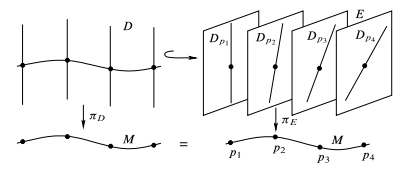
\includegraphics[width=\textwidth]{../\string_build/html/\string_images/subbundle.png}
\caption{Visualisierung eines Untervektorbündels, siehe \cite{Lee03} Kapitel 10.}\label{\detokenize{vektoranalysis/diffformen:fig-subbundle}}\end{figure}

\par
In diesem Fall erhält man also ein Untervektorbündel.
\begin{lemma}{}{vektoranalysis/diffformen:lemma-60}



\par
Sei \(\M\) eine glatte \(n\) dimesnionale Mannigfaltigkeit, dann ist \(\Lambda^k T^\ast\M\) ein glattes Untervektorbündel vom Rang \(\begin{pmatrix} n k \end{pmatrix}\).
\end{lemma}

\begin{proof}
 ToDo.
\end{proof}

\par
Dank der Bündelstruktur können wir erneut glatte Schnitte betrachten, welche nun auf das Konzept der Diffentialform führen.
\begin{definition}{}{vektoranalysis/diffformen:definition-61}



\par
Es sei \(\M\) eine glatte Mannigfaltigkeit, dann nennt man einen glatten Schnitt
\begin{align*}
\omega\in \Gamma(\Lambda^k T^\ast\M)
\end{align*}
\par
eine \(k\) Differentialform oder auch \(k\) Form. Den Vektorraum der Differntialformen notieren wir durch
\begin{align*}
\Omega^k(\M) := \Gamma(\Lambda^k T^\ast\M).
\end{align*}\end{definition}


\subsubsection{Das äußere Produkt}
\label{\detokenize{vektoranalysis/diffformen:das-auszere-produkt}}
\par
Eine Differentialform \(\omega\) auf \(U\subseteq\R^n\) ist eine von Ort zu Ort variierende äußere Form, deren Variation wir als glatt voraussetzen.

\par
Wir schreiben eine allgemeine \emph{\(k\)–Form} \(\omega\) in der \emph{Grundform}
\begin{align*}
\omega = \sum_{1\leq i_1<\ldots<i_k\leq n}\omega_{i_1\ldots i_k}
dx_{i_1}\wedge\ldots\wedge dx_{i_k}\in\Omega^k(U),
\end{align*}
\par
wobei
\begin{itemize}
\item {} 
\par
die \(\omega_{i_1\ldots i_k}\in \Omega^0(U):=C^\infty(U,\R)\), also glatte reelle Funktionen auf \(U\) sind,

\item {} 
\par
und die \(dx_i\) den Koordinatenfunktionen \(x_i:\R^n\to\R\) zugeordnete \(1\)–Differentialformen sind (\(dx_i\in\Omega^1(\R^n)\)).

\item {} 
\par
Den Raum der \(k\)–Differentialformen schreiben wir ab jetzt zur Unterscheidung vom Raum der äußeren \(k\)–Formen mit dem Symbol \(\Omega\) statt \(\Lambda\).

\end{itemize}

\par
Die \(dx_i\) sind durch ihre Wirkung auf ein Vektorfeld \(v:U\to
\R^n\) definiert, und \(dx_i(v)( y) := v_i( y)\).
\(1\)–Differentialformen machen also aus Vektorfeldern Funktionen, und für \(k\) Vektorfelder \(v^{(l)}:U\to\R^n\) ist für das \(\omega\) aus der Grundform
\begin{align*}
\omega\left(v^{(1)},\ldots,v^{(k)}\right) := \sum_{1\leq i_1<\ldots<i_k\leq n}
\omega_{i_1\ldots i_k}\cdot\det\begin{pmatrix} dx_{i_1}(v^{(1)})&\ldots& dx_{i_k}(v^{(1)})\\
\vdots&&\vdots\\
dx_{i_1}(v^{(k)})&\ldots& dx_{i_k}(v^{(k)}) \end{pmatrix}
\end{align*}
\par
definiert. Das Ergebnis ist also eine reelle Funktion auf \(U\).\textbackslash{}
Die Rechenregeln übertragen sich von den äußeren Formen auf die Differentialformten.

\par
Auf dem \(\R\)–Vektorraum
\begin{align*}
\Omega^*(U) := \bigoplus_{k=0}^n\Omega^k(U)
\end{align*}
\par
der Differentialformen betrachten wir jetzt
den \emph{Differentialoperator} \(d\), der durch
\begin{itemize}
\item {} 
\par
\(df := \sum_{i=1}^n\frac{\partial f}{\partial x_i}dx_i\) für Funktionen
\(f\in C^\infty(U,\R) = \Omega^0(U)\)

\item {} 
\par
und \(d\omega := \sum_{1\leq i_1<\ldots<i_k\leq n}d\omega_{i_1\ldots i_k}
\wedge dx_{i_1}\wedge\ldots\wedge dx_{i_k}\) für \(k\)–Formen \textbackslash{}linebreak
\(\omega = \sum_{1\leq i_1<\ldots<i_k\leq n}\omega_{i_1\ldots i_k}
dx_1\wedge\ldots\wedge dx_{i_k}\)

\end{itemize}

\par
definiert ist. \(d\) verwandelt eine \(k\)–Form also in eine \((k+1)\)–Form.
\begin{definition}{}{vektoranalysis/diffformen:aeussere Ableitung}



\par
Die lineare Abbildung \(d:\Omega^*(U)\to\Omega^*(U)\) heißt \href{https://de.wikipedia.org/wiki/\%C3\%84u\%C3\%9Fere\_Ableitung}{\textbf{äußere Ableitung}}.
\end{definition}
\begin{example}{}{vektoranalysis/diffformen:ex:10.14}


\begin{enumerate}

\item {} 
\par
Für \(\omega\in\Omega^0(\R^3)\) ist \(d\omega = \frac{\partial\omega}{\partial x_1}dx_1+
\frac{\partial\omega}{\partial x_2}dx_2+\frac{\partial\omega}{\partial x_3}dx_3\).

\item {} 
\par
Für \(\omega = \omega_1dx_1+\omega_2dx_2+\omega_3dx_3\in\Omega^1(\R^3)\) ist

\end{enumerate}
\begin{align*}
d\omega &=& (d\omega_1)\wedge dx_1+(d\omega_2)\wedge dx_2+(d\omega_3)\wedge
dx_3\\
&=& \left(\frac{\partial\omega_2}{\partial x_1}-\frac{\partial\omega_1}{\partial x_2}\right)
dx_1\wedge dx_2+ \left(\frac{\partial\omega_3}{\partial x_2}-\frac{\partial\omega_2}{\partial x_3}\right)
dx_2\wedge dx_3\\
&& + \left(\frac{\partial\omega_1}{\partial x_3}-\frac{\partial\omega_3}{\partial x_1}\right)
dx_3\wedge dx_1
\end{align*}\begin{enumerate}

\item {} 
\par
Für \(\omega = \omega_{12}dx_1\wedge dx_2+\omega_{23}dx_2\wedge dx_3
+\omega_{31}dx_3\wedge dx_1 \in\Omega^2(\R^3)\) ist

\end{enumerate}
\begin{align*}
d\omega = \left(\frac{\partial\omega_{12}}{\partial x_3} + \frac{\partial\omega_{23}}{\partial x_1}
+ \frac{\partial\omega_{31}}{\partial x_2}\right)dx_1\wedge dx_2\wedge dx_3.
\end{align*}\begin{enumerate}

\item {} 
\par
Für \(\omega\in\Omega^3(\R^3)\) ist \(d\omega=0\).

\end{enumerate}
\end{example}
\begin{theorem}{}{vektoranalysis/diffformen:Antiderivation}



\par
\(d\) ist eine \href{https://de.wikipedia.org/wiki/Derivation\_(Mathematik)\#Antiderivationen}{\textbf{Antiderivation}}, d.h. für \(\alpha\in\Omega^k(U)\) und \(\beta\in\Omega^l(U)\) ist
\begin{align*}
d(\alpha\wedge\beta) = (d\alpha)\wedge\beta+(-1)^k\alpha\wedge d\beta.
\end{align*}\end{theorem}

\begin{proof}
 Wegen der Linearität von \(d\) genügt es, diese Gleichung für Monome
\begin{align*}
\alpha := f\underbrace{dx_{i_1}\wedge\ldots\wedge dx_{i_k}}_{\tilde
{\alpha}},\ \beta := g\underbrace{dx_{j_1}\wedge\ldots\wedge dx_{j_l}}_
{\tilde{\beta}},\ f,g\in C^\infty(U,\R)
\end{align*}
\par
zu beweisen.
Es gilt
\begin{align*}
d(\alpha\wedge\beta) &=& d(f\cdot g)\tilde{\alpha}\wedge
\tilde{\beta} = \big((df)g+f(dg)\big)\,\tilde{\alpha}\wedge\tilde{\beta}\\
&=& (df)\tilde{\alpha}\wedge g\tilde{\beta}+ (-1)^kf\tilde{\alpha}
\end{align*}\end{proof}
\begin{theorem}{}{vektoranalysis/diffformen:thm:dd}



\par
Auf \(\Omega^*(U)\) gilt
\end{theorem}

\begin{proof}
 1. Für \(f\in\Omega^0(U)\) ist
\begin{align*}
ddf &=& d\left(\sum_{i=1}^n\frac{\partial f}
{\partial x_i}dx_i\right) = \sum_{i=1}^n\sum_{l=1}^n\frac{\partial^2f}{\partial x_l\partial x_i}
dx_l\wedge dx_i\\
& =& \sum_{1\leq r< s\leq n}\left(\frac{\partial^2 f}{\partial x_r
\partial x_s} - \frac{\partial^2f}{\partial x_s\partial x_r}\right)dx_r\wedge dx_s = 0,
\end{align*}
\par
da wir wegen der Glattheit von \(f\) die partiellen Ableitungen vertauschen
können.
\begin{enumerate}

\item {} 
\par
Für \(\omega = \sum\omega_{i_1\ldots i_k}dx_{i_1}\wedge\ldots\wedge dx_{i_k}
\in\Omega^k(U)\) ist\textbackslash{}

\end{enumerate}
\begin{align*}
dd\omega = \sum(\underbrace{dd\omega_{i_1\ldots i_k}}_0)
\wedge dx_{i_1}\wedge\ldots\wedge dx_{i_k} = 0,
\end{align*}
\par
denn gemäß Satz \cref{vektoranalysis/diffformen:Antiderivation} wird die äußere Ableitung auf die
1 Formen \(d\omega_{i_1\ldots i_k}\) und \(dx_{i_l}\) angewandt, und nach Teil 1.
ist das Ergebnis Null.
\end{proof}
\begin{definition}{}{vektoranalysis/diffformen:geschlossen:exakt}



\par
Eine Differentialform \(v\in\Omega^*(U)\) heißt
\begin{itemize}
\item {} 
\par
\textbf{geschlossen}, wenn \(dv=0\), *\textbf{exakt}, wenn \(v=d\psi\) für ein \(\psi\in\Omega^*(U)\) gilt.

\end{itemize}

\par
Nach Satz \cref{vektoranalysis/diffformen:thm:dd} sind exakte Differentialformen geschlossen.\textbackslash{} Für \(k\)–Formen auf konvexen offenen Teimengen \(U\subseteq \R^n\) gilt für \(k\ge 1\)auch die Umkehrung (sog.
\href{https://de.wikipedia.org/wiki/Poincar\%c3\%a9-Lemma}{\textbf{Poincaré Lemma}} ),  siehe Kapitel {sect:Poinca broken reference}).
\end{definition}


